\documentclass[11pt,landscape,a4paper]{article}
\usepackage[utf8]{inputenc}
\usepackage[ngerman]{babel}
\usepackage[T1]{fontenc}
\usepackage{tikz}
\usetikzlibrary{shapes,positioning,arrows,fit,calc,graphs,graphs.standard}
\usepackage[nosf]{kpfonts}
\usepackage[t1]{sourcesanspro}
\usepackage{multicol}
\usepackage{wrapfig}
\usepackage[top=2mm,bottom=2mm,left=2mm,right=2mm]{geometry}
\usepackage[framemethod=tikz]{mdframed}
\usepackage{microtype}
\usepackage{pdfpages}
\usepackage{soul}
\usepackage{enumitem}
\usepackage{multicol}
\usepackage[dvipsnames]{xcolor}
\usepackage[document]{ragged2e}
\usepackage{graphicx}

% math
\let\bar\overline
\everymath{\color{gray}}

% flowcharts
\tikzset{box/.style={draw, rectangle, thin, text centered, minimum height=0.1cm, minimum width=0.1cm}}
\tikzset{line/.style={draw, thin, -latex'}}

% bullets
\setitemize{noitemsep,topsep=0pt,parsep=0pt,partopsep=0pt,leftmargin=*}
\setenumerate{noitemsep,topsep=0pt,parsep=0pt,partopsep=0pt,leftmargin=*}
\setlength{\multicolsep}{0pt plus 0pt minus 0pt}

% line spacing
\renewcommand{\baselinestretch}{0.8}
\pagestyle{empty}

% no indentation
\makeatother
\setlength{\parindent}{0pt}

% section / subsection style
\makeatletter
\renewcommand{\section}{\@startsection{section}{1}{0mm}%
                                {.2ex}%
                                {.2ex}%x
                                {\color{ForestGreen}\sffamily\small\bfseries}}
\renewcommand{\subsection}{\@startsection{subsection}{1}{0mm}%
                                {.2ex}%
                                {.2ex}%x
                                {\color{olive}\sffamily\bfseries}}

\begin{document}
\footnotesize
\raggedright
\begin{multicols*}{3}
\section{Linear Algebra}
\subsection*{Semiring}
\emph{Monoid} ---
\begin{itemize}
    \item Consists of a set $\mathcal{A}$, an operation $*$, and an identity element $e$, such that:
    \begin{itemize}
        \item Associativity: $(a * b) * c = a * (b * c)$
        \item Identity: $a * e = e * a = a$
    \end{itemize}
    \item \emph{Commutative monoid}: Additionally commutative: $a * b = b * a$
\end{itemize}

{\color{lightgray}\hrule height 0.001mm}

\emph{Semiring} ---
\begin{itemize}
    \item $(\mathcal{A}, \oplus, \otimes, \overline{0}, \overline{1})$:
    \begin{itemize}
        \item $(\mathcal{A}, \oplus, \overline{0})$ is a commutative monoid
        \item $(\mathcal{A}, \otimes, \overline{1})$ is a monoid
        \item $\otimes$ distributes over $\oplus$:
        $
        (a \oplus b) \otimes c = (a \otimes c) \oplus (b \otimes c), \quad
        c \otimes (a \oplus b) = (c \otimes a) \oplus (c \otimes b)
        $
        \item $\overline{0}$ is an annihilator for $\otimes$:
        $
        a \otimes \overline{0} = \overline{0}, \quad \overline{0} \otimes a = \overline{0}
        $
    \end{itemize}
    \item \emph{Commutative semiring}: $\otimes$ is commutative: $a \otimes b = b \otimes a$
    \item \emph{Idempotent semiring}: $\oplus$ is idempotent: $a \oplus a = a$
    \begin{itemize}
        \item For idempotent semirings, $\bigoplus_{k=0}^{K} \boldsymbol{M}^k = ( \boldsymbol{I} + \boldsymbol{M})^{K}$\\
        Proof:
        \begin{itemize}
            \item Base case: $(\boldsymbol{I} \oplus \boldsymbol{M})^1 = \boldsymbol{I} \oplus \boldsymbol{M} = \boldsymbol{M}^0 \oplus \boldsymbol{M}^1 = \bigoplus_{k=0}^1 \boldsymbol{M}^k$
            \item Inductive step: $(\boldsymbol{I} \oplus \boldsymbol{M})^{K+1} = \left( \bigoplus_{k=0}^K \boldsymbol{M}^k \right) \otimes (\boldsymbol{I} \oplus \boldsymbol{M}) = \bigoplus_{k=0}^K (\boldsymbol{M}^k \otimes \boldsymbol{I}) \oplus \bigoplus_{k=0}^K (\boldsymbol{M}^k \otimes \boldsymbol{M}) = \bigoplus_{k=0}^K \boldsymbol{M}^k \oplus \bigoplus_{k=0}^K \boldsymbol{M}^{k+1} = \bigoplus_{k=0}^K \boldsymbol{M}^k \oplus \bigoplus_{k=1}^{K+1} \boldsymbol{M}^k$
            \item Because of idempotency, the repeated terms $ \boldsymbol{M}^k $ can be simplified ($ \boldsymbol{M}^k \oplus \boldsymbol{M}^k = \boldsymbol{M}^k$)
            \item Then, we have: $(\boldsymbol{I} \oplus \boldsymbol{M})^{K+1} = \bigoplus_{k=0}^{K+1} \boldsymbol{M}^k$
        \end{itemize}
        \item We can also show that, $ \bigoplus_{k=0}^{K} \boldsymbol{M}^k = \bigoplus_{k=0}^{K} \bigotimes_{n=0}^{\lfloor \log_2 N \rfloor} \boldsymbol{M}^{\alpha_n 2^n}$ if we use binary decomposition on matrix $\boldsymbol{M}$\\
        Proof:
        \begin{itemize}
            \item According to binary decomposition: $k = \sum_{n=0}^{\lfloor \log_2 N \rfloor} \alpha_n 2^n$ where $\alpha_n \in \{0, 1\}$ and $\alpha_n = 1$ if $2^n$ is part of the decomposition, otherwise $\alpha_n = 0$
            \item Then, $\boldsymbol{M}^k = \boldsymbol{M}^{\sum_{n=0}^{\lfloor \log_2 N \rfloor} \alpha_n 2^n} = \bigotimes_{n=0}^{\lfloor \log_2 N \rfloor} \boldsymbol{M}^{\alpha_n 2^n}$
        \end{itemize}
    \end{itemize}
    \item \emph{Closed semiring}: Additional unary operation: \emph{Kleene star} $*$ (\emph{asteration}):
    \begin{itemize}
        \item $
        x^* = \bigoplus_{n=0}^\infty x^{\otimes n} = \overline{1} \oplus x \oplus x^{\otimes 2} \oplus x^{\otimes 3} \oplus \cdots
        $
        \item Properties:
        $
        x^* = \overline{1} \oplus x \otimes x^* = \overline{1} \oplus x^* \otimes x
        $\\
        Proof:
        \begin{itemize}
            \item $ \overline{1} \oplus x \otimes x^* = \overline{1} \oplus x \otimes \left( \overline{1} \oplus x \oplus x^{\otimes 2} \oplus x^{\otimes 3} \oplus \cdots \right)$
            \item Using the distributive property of $ \oplus $ over $ \otimes $, we distribute $ x \otimes $ across the terms and get:
            $
            \overline{1} \oplus x \otimes x^* = \overline{1} \oplus x \oplus (x \otimes x) \oplus (x \otimes x^{\otimes 2}) \oplus (x \otimes x^{\otimes 3}) \oplus \cdots = \overline{1} \oplus x \oplus x^{\otimes 2} \oplus x^{\otimes 3} \oplus \cdots
            $
        \end{itemize}
        \item E.g.:
        \begin{itemize}
            \item For the log-sum-exp semiring, the Kleene star is the geometric series:
            $
            x^* = \log(\sum_{n=0}^\infty e^{n\times x}) = \log (\frac{1}{1 - e^x})$ for $x < 0$
            \item For the inside semiring and the first part of the expectation semiring, the Kleene star is the geometric series:
            $
            x^* = \sum_{n=0}^\infty x^n = \frac{1}{1 - x}$ for $x \in (0, 1)$\\
            Proof:
            $
            x^* = \frac{1}{1 - x} = 1 + \frac{1}{1 - x} -1 = 1 + \frac{1 - 1 + x}{1 - x} = 1 + \frac{x}{1 - x} = 1 + x \frac{1}{1 - x} = 1 + x x^*
            $
            \item For the Boolean semiring, the Kleene star is $
            x^* = 1$
        \end{itemize}
        \item As an alternative to Lehmann's algorithm, we can approximate Kleene star:
        $
        \sum_{k=0}^{K} \boldsymbol{M}^k \approx \boldsymbol{M}^*$ as $K \to \infty$ if $\rho(\boldsymbol{M}) < 1$ resp. $\sigma_{\max}(\boldsymbol{M}) = \| \boldsymbol{M} \|^2 < 1
        $, since then $\boldsymbol{M}^k \to 0$ as $k \to \infty$
        \item \emph{Truncation error} of this approximation:
        $
        || \boldsymbol{M}^* - \sum_{k=0}^K \boldsymbol{M}^k || \leq \frac{\sigma_{\max}(\boldsymbol{M})^{K+1}}{1 - \sigma_{\max}(\boldsymbol{M})}
        $\\
        Proof:
        \begin{itemize}
            \item $\boldsymbol{M}^* - \sum_{k=0}^K \boldsymbol{M}^k = \sum_{k=K+1}^\infty \boldsymbol{M}^k = \boldsymbol{M}^{K+1} \sum_{k=K+1}^\infty \boldsymbol{M}^{k-(K+1)} = \boldsymbol{M}^{K+1} \sum_{m=0}^\infty \boldsymbol{M}^m = \boldsymbol{M}^{K+1} \boldsymbol{M}^*$
            \item Then:
            $
            || \boldsymbol{M}^* - \sum_{k=0}^K \boldsymbol{M}^k || = || \boldsymbol{M}^{K+1} \boldsymbol{M}^* ||
            $
            \item Using the Cauchy-Schwarz inequality:
            $
            || \boldsymbol{M}^{K+1} \boldsymbol{M}^* || < || \boldsymbol{M}^{K+1} || \textrm{ } || \boldsymbol{M}^* ||
            $
            \item For $|| \boldsymbol{M}^{K+1} ||$:
            $
            || \boldsymbol{M}^{K+1} || \leq || \boldsymbol{M} ||^{K+1} = \sigma_{\max}(\boldsymbol{M})^{K+1}
            $
            \item For $|| \boldsymbol{M}^* ||$:
            $
            \sum_{n=0}^\infty || \boldsymbol{M}^n || \leq \sum_{n=0}^\infty || \boldsymbol{M} ||^n = \sum_{n=0}^\infty \sigma_{\max}(\boldsymbol{M})^n = \frac{1}{1 - \sigma_{\max}(\boldsymbol{M})}
            $ where the second-to-last term is a geometric series
            \item Then: $
            || \boldsymbol{M}^* - \sum_{k=0}^K \boldsymbol{M}^k || \leq \frac{\sigma_{\max}(\boldsymbol{M})^{K+1}}{1 - \sigma_{\max}(\boldsymbol{M})}
            $
        \end{itemize}
        \item Good approximation, especially if $\sigma_{\max} \ll 1$, since then the error becomes very small
        \item Runtime complexity exponential in $K$
    \end{itemize}
    \item \emph{$\overline{0}$-closed semiring}: $\overline{1} \oplus a = \overline{1}$
    \begin{itemize}
        \item Properties:
        \begin{itemize}
            \item $
            x^* = \bigoplus_{n=0}^{N-1} x^{\otimes n}$ since cycles in a path of length $\geq N$ do not contribute 
            \item Idempotent\\
            Proof:
            $a \oplus a = a \otimes (\overline{1} + \overline{1}) = a \otimes \overline{1} = a$ where the second last step follows due to defining property of $\overline{0}$-closed semiring 
        \end{itemize}
        \item E.g.: Tropical and arctic semiring
    \end{itemize}
\end{itemize}

Common semirings:
\begin{itemize}
    \item \emph{Boolean semiring}: $(\{0, 1\}, \lor, \land, 0, 1)$
    \item \emph{Inside semiring}: $(\mathbb{R} \cup \{\infty\}, +, \times, 0, 1)$
    \item \emph{Log-sum-exp semiring}: $(\mathbb{R} \cup \{-\infty\}, \oplus_{\textrm{log}}, +, -\infty, 0)$ where $a \oplus_{\textrm{log}} b = \log(e^a + e^b)$
    \item \emph{Viterbi semiring}: $([0,1], \max, \times, 0,1)$ (for original Viterbi algorithm) or $(\mathbb{R}, \max, \times, 0,1)$ (for syntactic parsing)
    \item \emph{Arctic semiring}: $(\mathbb{R} \cup \{-\infty\}, \max, +, -\infty, 0)$
    \item \emph{Tropical semiring}: $(\mathbb{R} \cup \{\infty\}, \min, +, \infty, 0)$
    \item \emph{Language semiring}: $(2^{\Sigma^*}, \cup, \circ, \{\}, \{\epsilon\})$ where $2^{\Sigma^*}$ is the set of all possible languages and $A \circ B = \{a \circ b \mid a \in A, b \in B\}$ is the concatenation
    \item \emph{Expectation semiring}: $
    ( \langle \mathbb{R} \times \mathbb{R} \rangle, \oplus, \otimes, \overline{0}, \overline{1} )
    $ where:
    \begin{itemize}
        \item
        $
        \langle x, y \rangle \oplus \langle x', y' \rangle = \langle x + x', y + y' \rangle
        $
        \item $
        \langle x, y \rangle \otimes \langle x', y' \rangle = \langle x \cdot x', x \cdot y' + x' \cdot y \rangle$
        \item $\overline{0} = \langle 0,0 \rangle$
        \item $\overline{1} = \langle 1,0 \rangle$
    \end{itemize}
\end{itemize}

{\color{black}\hrule height 0.001mm}

\subsection*{Other}
\emph{Common exp and log rules} ---
\begin{multicols}{2}
\begin{itemize}
    \item $a^m \cdot a^n = a^{m+n}$
    \item $\frac{a^m}{a^n} = a^{m-n}$
    \item $(ab)^n = a^n b^n$
    \item $\left(\frac{a}{b}\right)^n = \frac{a^n}{b^n}$
    \item $a^{-n} = \frac{1}{a^n}$
    \item $a^0 = 1$
    \item $a^1 = a$
    \item $\log(xy) = \log x + \log y$
    \item $\log\left(\frac{x}{y}\right) = \log x - \log y$
    \item $\log(x^n) = n \log x$
    \item $\log 1 = 0$
    \item $\log (x<1) < 0$
    \item $\log (x>1) > 0$
    \item $e^{log(x)} = log(e^x) = x$
\end{itemize}
\end{multicols}

{\color{lightgray}\hrule height 0.001mm}

\emph{Geometric series} --- 
\begin{itemize}
    \item Finite: $S_n = \sum_{i=1}^n a_i r^{i-1} = a_1 (\frac{1-r^n}{1-r})$
    \item Infinite: $S = \sum_{i=0}^\infty a_i r^i = \frac{a_1}{1-r}$ for $r < 1$
\end{itemize}
\section{Calculus}
\subsection*{Derivatives}
\emph{Rules} --- 
\begin{itemize}
    \item Sum rule: $\frac{\partial f + g}{\partial x} = \frac{\partial f}{\partial x} + \frac{\partial g}{\partial x}$
    \item Product rule: $\frac{\partial f \times g}{\partial x} = f \times \frac{\partial g}{\partial x} + g \times \frac{\partial f}{\partial x}$
    \item Chain rule: $\frac{\partial f(g)}{\partial x} = \frac{\partial f}{\partial g} \times \frac{g}{\partial x}$
    \item Scalar multipliers of the whole gradient can be ignored, even if the variable we are deriving wrt is included in this scalar
\end{itemize}

{\color{lightgray}\hrule height 0.001mm}

\emph{Common derivatives} --- 
\begin{multicols}{2}
\begin{itemize}
    \item $\frac{\partial x^n}{\partial x} = nx^{n-1}$
    \item $\frac{\partial e^{kx}}{\partial x} = k \times e^{kx}$
    \item $\frac{\partial log(x)}{\partial x} = \frac{1}{x}$
    \item $\frac{\partial \sqrt{x}}{\partial x} = \frac{1}{2\sqrt{x}}$
    \item $\frac{\partial \sin(x)}{\partial x} = \cos(x)$
    \item $\frac{\partial \cos(x)}{\partial x} = -\sin(x)$
\end{itemize}
\end{multicols}

{\color{lightgray}\hrule height 0.001mm}

\emph{Partial and directional derivative} --- 
\begin{itemize}
    \item For a function that depends on $n$ variables $\{x_i\}_{i=2}^n$, partial derivative is slope of tangent line along direction of one specific variable $x_i$
    \item Directional derivative is slope of tangent line along direction of selected unit vector $\boldsymbol{u}$
\end{itemize}

{\color{lightgray}\hrule height 0.001mm}

\emph{Gradient} --- 
\begin{itemize}
    \item Given scalar-valued function $f: \mathbb{R}^{n} \rightarrow \mathbb{R}$, returns vector containing first-order partial derivatives:\\
    $\nabla_{\boldsymbol{x}} f: [\frac{\partial f}{\partial x_1} ... \frac{\partial f}{\partial x_n}]^\intercal$
    \item Gradient points in direction of greatest upward slope of f \item Magnitude of gradient equals rate of change when moving into direction of greatest upward slope 
\end{itemize}

{\color{lightgray}\hrule height 0.001mm}

\emph{Hessian} --- 
\begin{itemize}
    \item Given scalar-valued function $f: \mathbb{R}^{n} \rightarrow \mathbb{R}$, returns matrix containing second-order partial derivatives:\\
    $\mathcal{H} = \nabla_{\boldsymbol{x}}^2 f: \begin{bmatrix}
    \frac{\partial^2 f}{\partial x_1^2} & ... & \frac{\partial^2 f}{\partial x_1 \partial x_n} \\
    ... & ... & ... \\
    \frac{\partial^2 f}{\partial x_n \partial x_1} & ... & \frac{\partial^2 f}{\partial x_n^2}
    \end{bmatrix}$
    \item $\mathcal{H}$ is symmetric 
\end{itemize}

{\color{lightgray}\hrule height 0.001mm}

\emph{Jacobian} --- 
\begin{itemize}
    \item Given vector-valued function $\boldsymbol{f}: \mathbb{R}^{n} \rightarrow \mathbb{R}^{m}$ with $\boldsymbol{f} = [f_1(\boldsymbol{x}), ..., f_m(\boldsymbol{x})]^\intercal$, returns matrix containing first-order partial derivatives:\\
    $\nabla_{\boldsymbol{x}} \boldsymbol{f}: \begin{bmatrix}
    \frac{\partial f_1}{\partial x_1} & ... & \frac{\partial f_1}{\partial x_n} \\
    ... & ... & ... \\
    \frac{\partial f_m}{\partial x_1} & ... & \frac{\partial f_m}{\partial x_n}
    \end{bmatrix} \in \mathbb{R}^{m \times n}$
\end{itemize}

{\color{lightgray}\hrule height 0.001mm}

\emph{Matrix calculus rules} --- 
\begin{multicols}{2}
\begin{itemize}
    \item $\frac{\partial \boldsymbol{a}^\intercal\boldsymbol{x}}{\partial \boldsymbol{x}} = \boldsymbol{a}$
    \item $\frac{\partial \boldsymbol{x}^\intercal\boldsymbol{A}\boldsymbol{x}}{\partial \boldsymbol{x}} = (\boldsymbol{A} + \boldsymbol{A}^\intercal)\boldsymbol{x}$
    \item $\frac{\partial \boldsymbol{a}^\intercal\boldsymbol{A}\boldsymbol{b}}{\partial \boldsymbol{A}} = \boldsymbol{a}\boldsymbol{b}^\intercal$
    \item For symmetric $\boldsymbol{A}$: $\frac{\partial \boldsymbol{x}^\intercal\boldsymbol{A}\boldsymbol{x}}{\partial \boldsymbol{x}} = 2\boldsymbol{A}\boldsymbol{x}$
    \item For square $\boldsymbol{A}$: 
    \begin{itemize}
        \item $\frac{\partial \boldsymbol{a}^\intercal\boldsymbol{A}^{-1}\boldsymbol{b}}{\partial \boldsymbol{A}} = -(\boldsymbol{A}^\intercal)^{-1} \boldsymbol{a}\boldsymbol{c}^\intercal (\boldsymbol{A}^\intercal)^{-1}$
        \item $\frac{\partial log(|\boldsymbol{A}|)}{\partial \boldsymbol{A}} = (\boldsymbol{A}^\intercal)^{-1}$
    \end{itemize}
\end{itemize}
\end{multicols}

{\color{black}\hrule height 0.001mm}

\subsection*{Extrema}
\emph{Conditions for local minima and maxima} --- 
\begin{itemize}
    \item Point is a stationary point, i.e. first-order derivative = 0
    \item If Hessian is pd, it's a local minimum, if Hessian is nd, it's a local maximum, if Hessian is indefinite, it's a saddle point
    \item Local minima and maxima are the unique global minima and maxima in strictly convex functions resp. one of possibly infinitely many global minima and maxima in convex functions
\end{itemize}

{\color{lightgray}\hrule height 0.001mm}

\emph{Convexity} --- 
\begin{itemize}
    \item For a convex function: 
    \begin{itemize}
        \item $f(\lambda x + (1-\lambda)y \leq \lambda f(x) + (1-\lambda) f(y)$ with $\lambda \in [0,1]$
        \item Hessian of stationary point(s) is psd
        \item Global minimum exists, but may not be unique
    \end{itemize}
    \item For a strictly convex function:
    \begin{itemize}
        \item $f(\lambda x + (1-\lambda)y < \lambda f(x) + (1-\lambda) f(y)$ with $\lambda \in [0,1]$
        \item Hessian of stationary point is pd
        \item Unique global minimum exists 
    \end{itemize}
    \item Sum of convex functions $f_2(x) + f_1(x)$ is also convex, sum of convex and strictly convex function is strictly convex
    \item Chain of convex functions $f_2(f_1(x))$, where outer function $f_2(x)$ is increasing, is also convex
    \item Scalar multiple of convex function $\lambda f(x)$, where $\lambda \geq 0$, is also convex
    \item Any norm is convex
\end{itemize}

{\color{lightgray}\hrule height 0.001mm}

\emph{Nature of optimum} --- 
What does Hessian and function look like?
\begin{itemize}
    \item If Hessian is pd and loss function is strictly convex, stationary point is a global minimum, and there is a unique solution
    \item If Hessian is psd and loss function is convex, stationary point is a global minimum, and there may be a geometrically unique or infinitely many solutions
    \item If Hessian is p(s)d but loss function is not convex, stationary point may be a local minimum and there may be a geometrically unique or infinitely many solutions
\end{itemize}

{\color{lightgray}\hrule height 0.001mm}

\emph{Optimization approach} --- 
Is function differentiable, continuous, and are relevant terms invertible?
\begin{itemize}
    \item If yes, analytically solvable
    \item If no, numerically solvable (e.g. via gradient descent)
\end{itemize}

{\color{lightgray}\hrule height 0.001mm}

\emph{Constrained optimization} --- 
\begin{itemize}
    \item \emph{Lagrangian function}: $\mathcal{L}(\boldsymbol{x},\lambda) = f(\boldsymbol{x}) + \lambda g(\boldsymbol{x})$, where $g(\boldsymbol{x})$ is an $(m-1)$ dimensional constraint surface and $\lambda$ is the Lagrange multiplier
    \item$\nabla_{\boldsymbol{x}} \mathcal{L} = \nabla_{\boldsymbol{x}} f(\boldsymbol{x}) + \lambda \nabla_{\boldsymbol{x}} g(\boldsymbol{x})$
    \item$\nabla_{\lambda} \mathcal{L} = g(\boldsymbol{x})$
    \item Solution is feasible if it fulfills constraints and optimal, if no other feasible solution produces a lower error
    \item Minimizing over Lagrangian $\mathcal{L}(\boldsymbol{x},\lambda) = f(\boldsymbol{x}) + \lambda g(\boldsymbol{x})$ corresponds to minimizing log-loss:
    \begin{itemize}
        \item $\hat{\boldsymbol{x}} = \arg\max_\boldsymbol{x} p(\boldsymbol{D} |\boldsymbol{x}) \rho(\boldsymbol{x}) $ 
        \item $= \arg\min_\boldsymbol{x} (- log p(\boldsymbol{D} |\boldsymbol{x}) + k(\boldsymbol{x}))$
        \item where $k(\boldsymbol{x}) = -log \rho(\boldsymbol{x})$
    \end{itemize}
    $\mathcal{L}(\boldsymbol{x},\lambda) = f(\boldsymbol{x}) + \lambda g(\boldsymbol{x})$
\end{itemize}\\
For equality constraints: Minimize $f(\boldsymbol{x})$ subject to $g(\boldsymbol{x}) = 0$
\begin{itemize}
    \item Gradient of $f(\boldsymbol{x})$ must be orthogonal to constraint surface, otherwise (if it points into any direction along the constraint surface) $f(\boldsymbol{x})$ could still decrease for movements along the constraint surface
    \item On the constraint surface, $g(\boldsymbol{x})$ is a constant, so moving along any direction on the constraint surface has a directional derivative of 0. Since the gradient of $g(\boldsymbol{x})$ points into the direction of steepest ascent, it must be orthogonal to the constraint surface, otherwise (if it points into any direction along the constraint surface) $g(\boldsymbol{x})$ would not be constant on the constraint surface
    \item Then, gradients are parallel at optimum: $\nabla_{\boldsymbol{x}} f(\boldsymbol{x^*}) = \lambda \times \nabla_{\boldsymbol{x}} g(\boldsymbol{x^*})$
    \item To find $\boldsymbol{x^*}$ and $\lambda^*$: 
    \begin{itemize}
        \item $\nabla_{\boldsymbol{x}} \mathcal{L} = 0$, expresses parallelity condition at minimum $\boldsymbol{x^*}$
        \item $\nabla_{\lambda} \mathcal{L} = 0$, expresses constraint
        \item This is an unconstrained optimization problem
    \end{itemize}
    \item Optimum $\boldsymbol{x^*}$ and $\lambda^*$ represents a saddle point of $\mathcal{L}$
\end{itemize}\\
For inequality constraints: Minimize $f(\boldsymbol{x})$ subject to $g(\boldsymbol{x}) \leq 0$ 
\begin{itemize}
    \item If $\boldsymbol{x^*}$ lies in $g(\boldsymbol{x}) < 0$, constraint is inactive
    \item Otherwise, if $\boldsymbol{x^*}$ lies in $g(\boldsymbol{x}) = 0$, constraint is active:
    \begin{itemize}
        \item Gradient of $f(\boldsymbol{x})$ must point towards $g(\boldsymbol{x}) < 0$ region, otherwise (if it would point away from $g(\boldsymbol{x}) < 0$ region) the optimum would lie in this region
        \item Then, gradients are anti-parallel at optimum: $\nabla_{\boldsymbol{x}} f(\boldsymbol{x^*}) = -\lambda \times \nabla_{\boldsymbol{x}} g(\boldsymbol{x^*})$
    \end{itemize}
    \item To find $\boldsymbol{x^*}$ and $\lambda^*$: 
    \begin{itemize}
        \item $\nabla_{\boldsymbol{x}} \mathcal{L} = 0$ subject to \emph{Karush Kuhn Tucker conditions}:
        \begin{itemize}
            \item $g(\boldsymbol{x}) \leq 0$
            \item $\lambda \geq 0$
            \item \emph{Complementary slackness condition}: $\lambda g(\boldsymbol{x}) = 0$, with $\lambda = 0, g(\boldsymbol{x}) < 0$ for inactive constraints and $\lambda > 0, g(\boldsymbol{x}) = 0$ for active constraints
        \end{itemize}
        \item $\nabla_{\lambda} \mathcal{L} = 0$ given complementary slackness condition
        \item This is not an unconstrained optimization problem, but can be solved via duality
    \end{itemize}
    \item Optimum $\boldsymbol{x^*}$ and $\lambda^*$ represents a saddle point of $\mathcal{L}$
\end{itemize}\\
For multiple constraints: Minimize $f(\boldsymbol{x})$ subject to $m$ inequality constraints $\{g^{(i)}(\boldsymbol{x}) \leq 0\}_{i=1}^m$ and $p$ equality constraints $\{h^{(j)}(\boldsymbol{x}) = 0\}_{j=1}^p$ 
\begin{itemize}
    \item Then, Lagrangian is given by: $\mathcal{L}(\boldsymbol{x},\boldsymbol{\lambda},\boldsymbol{\mu}) = f(\boldsymbol{x}) + \sum_{i=1}^m \mu^{(i)} g^{(i)}(\boldsymbol{x}) + \sum_{j=1}^p \lambda^{(j)} h^{(j)}(\boldsymbol{x})$
    \item Then, general solution $\boldsymbol{x^*},\boldsymbol{\lambda^*},\boldsymbol{\mu^*}$ is given by: $\nabla_{\boldsymbol{x}} \mathcal{L} = 0$ subject to:
    \begin{itemize}
        \item $\{g^{(i)}(\boldsymbol{x}) \leq 0\}_{i=1}^m$ and $\{h^{(j)}(\boldsymbol{x}) = 0\}_{j=1}^p$ 
        \item $\{\mu^{(i)} \geq 0\}_{i=1}^m$
        \item $\{\mu^{(i)}g^{(i)}(\boldsymbol{x}) = 0\}_{i=1}^m$
    \end{itemize}
\end{itemize}\\
\emph{Primal problem}:
\begin{itemize}
    \item $\textrm{min}_{\boldsymbol{x}} [\textrm{max}_{\boldsymbol{\lambda},\boldsymbol{\mu}} \mathcal{L}]$
    \item $\textrm{max}_{\boldsymbol{\lambda},\boldsymbol{\mu}} \mathcal{L} = f(\boldsymbol{x}) + \textrm{max}_{\boldsymbol{\lambda},\boldsymbol{\mu}} [\sum_{i=1}^m \mu^{(i)} g^{(i)}(\boldsymbol{x}) + \sum_{j=1}^p \lambda^{(j)} h^{(j)}(\boldsymbol{x})]$
    \item Second term gives rise to barrier function:
    \begin{itemize}
        \item $= 0$ subject to constraints being met, given complementary slackness condition for inequality constraints and $h^{(j)}(\boldsymbol{x}) = 0$ for equality constraints, which implies that dual problem becomes $\textrm{min}_{\boldsymbol{x}}(f(\boldsymbol{x}))$
        \item $= \infty$ otherwise, which implies that primal problem cannot be solved
    \end{itemize}
    \item Let $f(\boldsymbol{x}^*)$ be the solution to the primal problem
\end{itemize}
Solving inequality constraints via duality: 
\begin{itemize}
    \item \emph{Dual problem}: $ \textrm{max}_{\boldsymbol{\lambda},\boldsymbol{\mu}} [\textrm{min}_{\boldsymbol{x}} \mathcal{L}]$
    \item Let $\textrm{min}_{\boldsymbol{x}} \mathcal{L} = \theta(\boldsymbol{\lambda},\boldsymbol{\mu})$
    \item Let $\theta(\boldsymbol{\lambda}^*,\boldsymbol{\mu}^*)$ be the solution to the dual problem
\end{itemize}
\emph{Weak duality}:
\begin{itemize}
    \item Weak duality always holds and gives a lower bound of minimum of primal problem
    \item Given minimax theorem, $f(\boldsymbol{x}^*) = \textrm{min}_{\boldsymbol{x}} [\textrm{max}_{\boldsymbol{\lambda},\boldsymbol{\mu}} \mathcal{L}] = \textrm{min}_{\boldsymbol{x}}(f(\boldsymbol{x})) \textrm{ (provided barrier function) } \geq \textrm{max}_{\boldsymbol{\lambda},\boldsymbol{\mu}} [\textrm{min}_{\boldsymbol{x}} \mathcal{L}] = \theta(\boldsymbol{\lambda}^*,\boldsymbol{\mu}^*)$
    \item $\textrm{min}_{\boldsymbol{x}} \mathcal{L}$ is an unconstrained optimization problem 
    \item $\textrm{max}_{\boldsymbol{\lambda},\boldsymbol{\mu}} [\textrm{min}_{\boldsymbol{x}} \mathcal{L}]$ is a concave maximization problem 
\end{itemize}
\emph{Strong duality}:
\begin{itemize}
    \item Strong duality holds under certain conditions, for example \emph{Slater's condition} if there exists a solution that strictly fulfills all constraints $\{g^{(i)}(\boldsymbol{x}) < 0\}_{i=1}^m$ and $\{h^{(j)}(\boldsymbol{x}) < 0\}_{j=1}^p$
    \item Then, $f(\boldsymbol{x}^*) = \textrm{min}_{\boldsymbol{x}} [\textrm{max}_{\boldsymbol{\lambda},\boldsymbol{\mu}} \mathcal{L}] = \textrm{max}_{\boldsymbol{\lambda},\boldsymbol{\mu}} [\textrm{min}_{\boldsymbol{x}} \mathcal{L}]= \theta(\boldsymbol{\lambda}^*,\boldsymbol{\mu}^*)$
    \item $\textrm{min}_{\boldsymbol{x}} \mathcal{L}$ can be solved for general solution $\boldsymbol{x^*}$ in terms of $\boldsymbol{\lambda},\boldsymbol{\mu}$
    \item Plug $\boldsymbol{x^*}$ back into $\mathcal{L}$ and maximize to find solutions $\boldsymbol{\lambda^*},\boldsymbol{\mu^*}$
    \item Specify $\boldsymbol{x^*}$ based on $\boldsymbol{\lambda^*},\boldsymbol{\mu^*}$
\end{itemize}

{\color{black}\hrule height 0.001mm}

\subsection*{Integrals}
\emph{Indefinite integral} --- 
\begin{itemize}
    \item $F(x) = \int f(x) dx$
    \item $F'(x) = f(x)$
\end{itemize}

{\color{lightgray}\hrule height 0.001mm}

\emph{Definite integral} --- 
\begin{itemize}
    \item $F(b) - F(a) = \int_a^b f(x) dx$
    \item $F'(x) = f(x)$
\end{itemize}

{\color{lightgray}\hrule height 0.001mm}

\emph{Common integrals} --- 
\begin{itemize}
    \item $f(x) = x^n \rightarrow F(x) = \frac{x^{n+1}}{n+1}$ for $n \neq 1$
    \item $f(x) = \frac{1}{x} \rightarrow F(x) = log(x)$
    \item $f(x) = e^x \rightarrow F(x) = e^x$
\end{itemize}
\section{Probability and Statistics}
\subsection*{Terminology}
\emph{Kolmogorov axioms} --- 
Probability space defined by:
\begin{itemize}
    \item Sample space: All possible outcomes $\Omega = \{\omega_1,...,\omega_n\}$
    \item Event space: All possible results, where an event is a subset of the sample space 
    \item Probability measure: Function that assigns a probability to an event 
\end{itemize}
Axioms:
\begin{itemize}
    \item Event space must be a \emph{sigma algebra}:
    \begin{itemize}
        \item If $A$ is in sample space with $P = a$, its complement is also in sample space with $P = 1-a$
        \item If $A_1,...A_n$ are in sample space with $P=a_1, ..., a_n$, their union is also in sample space with $P = a_1 + ... + a_n$
    \end{itemize}
    \item Probability measure must satisfy:
    \begin{itemize}
        \item $0 \leq \mathbb{P}(A) \leq 1$
        \item $\mathbb{P}({\Omega}) = 1$
        \item If $A_1,A_2,...$ are in sample space and do not intersect, then $\mathbb{P}(A_1 \cup A_2 \cup ...) = \int_{n=1}^{\infty} \mathbb{P}(A_n)$
    \end{itemize}
\end{itemize}
Further properties:
\begin{itemize}
    \item All sets than can be formed from left and right inclusive interval $[0,a]$ are events. On that basis:
    \begin{itemize}
        \item $(a,1] = [0,a]^c \in$ event space, with $P = 1 - a$
        \item $(a,b] = ([0,a] \cup (b,1])^c = ([0,a] \cup [0,b]^c)^c \in$ event space, with $P = 1 - (a + 1 - b) = 1 - a - 1 + b = b - a$
        \item $\{0\} \in$ event space, with $P = 0$
        \item $\{a\} \in$ event space, with $P = 0$
        \item $[a,b] = \{a\} \cup (a,b] = \{a\} \cup ([0,a] \cup [0,b]^c)^c \in$ event space, with $P = 0 + b - a$
        \item $[a,b) = [a,b] \backslash \{b\} = ([0,a] \cup [0,b]^c)^c \backslash \{b\} \in$ event space, with $P = b - a - 0$
    \end{itemize}
\end{itemize}

{\color{lightgray}\hrule height 0.001mm}

\emph{Variables} --- 
\begin{itemize}
    \item Random variable:
    \begin{itemize}
        \item Discrete random variable: Characterized by pmf
        \item Continuous random variable: Characterized by pdf
    \end{itemize}
    \item Independent random variables:
    \begin{itemize}
        \item $\mathbb{P}(A|B) = \mathbb{P}(A)$ and $\mathbb{P}(B|A) = \mathbb{P}(B)$
        \item From this follows that $f_{A|B}(a|b) = f_A(a)$ and $\mathbb{E}(A|B) = \mathbb{E}(A)$ 
        \item $\mathbb{P}(A \cap B) = \mathbb{P}(A)\mathbb{P}(B)$
        \item From this it follows that $f_{A,B}(a,b) = f_A(a) f_B(b)$ and $\mathbb{E}(A,B) = \mathbb{E}(A)\mathbb{E}(B)$
        \item Correlation is 0 
        \item Functions of independent random variables are also independent
    \end{itemize}
    \item Conditionally independent random variables: Two random variables $\mathcal{X}$ and $\mathcal{Y}$ are conditionally independent, if there is a confounder $\mathcal{L}$ that causally affects both variables, but if we control for this confounder, the variables are not causally connected
    \item I.I.D. random variables: Independent and from identical distribution
\end{itemize}

{\color{lightgray}\hrule height 0.001mm}

\emph{Events} --- 
\begin{itemize}
    \item Complement: $\mathbb{P}(A^C) = 1 - \mathbb{P}(A)$ and $\mathbb{P}(A \cup A^C) = \mathbb{P}(A)\mathbb{P}(A^C)$
    \item Disjoint / mutually exclusive vs. joint / mutually inclusive
    \item Subset $A \subset B$ with $\mathbb{P}(A) < \mathbb{P}(B)$
\end{itemize}

{\color{lightgray}\hrule height 0.001mm}

\emph{Probabilities} --- 
\begin{itemize}
    \item Marginal probability $\mathbb{P}(A)$: Probability for single variable: $p(\mathcal{X}) = \sum_{\mathcal{Y}}p(x,y)$ resp. $f(\mathcal{X}) = \int_{\mathcal{Y}}f(x,y)dy$
    \item Joint probability $\mathbb{P}(A \cap B)$: Probability for combination of variables, given by all possible combinations resp. convolution of their pdfs 
    \item Conditional probability $\mathbb{P}(A|B) = \frac{\mathbb{P}(A \cap B)}{\mathbb{P}(B)}$: Probability for variable, given other variable: $p(\mathcal{X}|\mathcal{Y}) = \frac{p(x,y)}{\sum_{\mathcal{X}}p(x,y)}$ resp. $f(\mathcal{X}|\mathcal{Y}) = \frac{f(x,y)}{\int_{\mathcal{X}}f(x,y)dy}$
    \begin{itemize}
        \item $\mathbb{P}(A|B) = 1 - \mathbb{P}(A^C|B)$
        \item $\mathbb{P}(A_1|B) + \mathbb{P}(A_2|B) + ... = 1$
        \item If conditioning on subset $S$:
        \begin{align*}
        p(x | S) = 
        \left\{
            \begin{aligned}
                 & p(x) / p(x \in S) \quad & x \in S \\ 
                 & 0 \quad & x \notin S  
            \end{aligned}
        \right.
        \end{align*}
    \end{itemize}
    \item Bayesian terminology: 
    \begin{itemize}
        \item Prior $\mathbb{P}(\textrm{parameter})$
        \item Posterior $\mathbb{P}(\textrm{parameter} | \textrm{data})$
        \item Likelihood $\mathbb{P}(\textrm{data} | \textrm{parameter})$
        \item Evidence $\mathbb{P}(\textrm{data})$
    \end{itemize}
    \item \emph{Bayes theorem}: $\textrm{Posterior } \mathbb{P}(A|B) = \frac{\textrm{Likelihood }\mathbb{P}(B|A) \times  \textrm{Prior }\mathbb{P}(A)}{\textrm{Evidence }\mathbb{P}(B)}$
    \item Attention! In $p(\cdot | \theta)$ the $|$ can either refer to parametrizing on $\theta$ (parameter is part of the distribution's form but isn't observed or fixed) or conditioning on $\theta$ (parameter takes a observed and fixed value, and we evaluate the distribution on this condition)
\end{itemize}

{\color{black}\hrule height 0.001mm}

\subsection*{Measures}
\emph{$n^{th}$ moment} --- 
$\mathbb{E}(\mathcal{X}^n) = \int_{-\infty}^{\infty}x^n \times f(x)dx$

{\color{lightgray}\hrule height 0.001mm}

\emph{Expected value} --- 
$\mathbb{E}(\mathcal{X}) = \sum_{\mathcal{X}}x \times p(x)$ resp. $\mathbb{E}(\mathcal{X}) = \int_{-\infty}^{\infty}x \times f(x)dx$ with pmf resp. pdf --- Properties:
\begin{multicols}{2}
\begin{itemize}
    \item $\mathbb{E}(\alpha)=\alpha$
    \item $\mathbb{E}(\alpha\mathcal{X}+\beta)=\alpha\mathbb{E}(\mathcal{X})+\beta$
    \item $\mathbb{E}(\alpha\mathcal{X} + \beta\mathcal{Y})=\alpha\mathbb{E}(\mathcal{X})+\beta\mathbb{E}(\mathcal{Y})$
    \item For orthogonal variables:
    \begin{itemize}
        \item  $\mathbb{E}(\mathcal{X}\mathcal{Y})=0$
        \item $\mathbb{E}((\mathcal{X}+\mathcal{Y})^2)=\mathbb{E}(\mathcal{X}^2) + \mathbb{E}(\mathcal{Y}^2)$
    \end{itemize}
    \item For independent variables: $\mathbb{E}(\mathcal{X}\mathcal{Y})=\mathbb{E}(\mathcal{X})\mathbb{E}(\mathcal{Y})$
    \item For vector $\boldsymbol{y} = \boldsymbol{A}\boldsymbol{x}$:\\
    $\mathbb{E}_y(\boldsymbol{A}\boldsymbol{x})=\boldsymbol{A}\mathbb{E}_X(\boldsymbol{x})$
\end{itemize}
\end{multicols}
\begin{itemize}
    \item For conditional probability ($A$ is an event, $X$ is a random variable): \\
    \begin{itemize}
        \item $\mathbb{E}[P(X | A)] = \sum_x P(X=x) \times P(X=x | A) $ resp. $\int_{-\infty}^{\infty} f_X(x) \times f_{X|A}(x)dx$ 
        \item $\mathbb{E}[P(A | X)] = P(A) = \sum_x P(X=x) \times P(A | X=x) $ resp. $\int_{-\infty}^{\infty} f_X(x) \times P(A|X=x) dx$ 
    \end{itemize}
    \item For conditional events resp. variables ($A$ is an event, $X$ is a random variable): \\
    \begin{itemize}
        \item $\mathbb{E}(X | A) = \sum_x x \times P(X=x | A) $ resp. $\int_{-\infty}^{\infty} x \times f_{X|A}(x)dx$ 
        \item $\mathbb{E}(A | X) = P(A|X)$
        \item $\mathbb{E}[\mathbb{E}(X | A)] = \mathbb{E}(X)$\\
        Proof:
        \begin{itemize}
            \item $\mathbb{E}[\mathbb{E}(X | A)] = \int_{-\infty}^{\infty} f_A(a) \mathbb{E}(X | A) da = \int_{-\infty}^{\infty} f_A(a) \int_{-\infty}^{\infty} x f_{X|A}(x|a) dx da = \int_{-\infty}^{\infty} \int_{-\infty}^{\infty} x f_{X,A}(x,a) dx da = \int_{-\infty}^{\infty} x \int_{-\infty}^{\infty} f_{X,A}(x,a) da dx = \int_{-\infty}^{\infty} x f_{X}(x) dx = \mathbb{E}(X)$
        \end{itemize}
    \end{itemize}
    \item \emph{Cauchy Schwarz inequality}: $\mathbb{E}(\mathcal{X},\mathcal{Y})^2 \leq \mathbb{E}(\mathcal{X}^2)\mathbb{E}(\mathcal{Y}^2)$
\end{itemize}

{\color{lightgray}\hrule height 0.001mm}

\emph{Median} --- Real number $M$ defined by $P(X<M) = P(X>M)$

{\color{lightgray}\hrule height 0.001mm}

\emph{Standard deviation} --- $\sqrt{\mathbb{V}(\mathcal{X})}$

{\color{lightgray}\hrule height 0.001mm}

\emph{Covariance} ---
\begin{itemize}
    \item Univariate variance of a random variable: $\mathbb{V}(\mathcal{X}) = \mathbb{E}((\mathcal{X}-\mathbb{E}(\mathcal{X}))^2) = \mathbb{E}(\mathcal{X}^2) - \mathbb{E}(\mathcal{X})^2$ where $\mathbb{E}(\mathcal{X}^2)$ is the unnormalized correlation resp. inner product
    \item Univariate covariance of two random variables: $\textrm{Cov}(\mathcal{X}, \mathcal{Y}) = \mathbb{E}((\mathcal{X}-\mathbb{E}(\mathcal{X}))(\mathcal{Y}-\mathbb{E}(\mathcal{Y}))) = \mathbb{E}(\mathcal{X}\mathcal{Y}) - \mu_{\mathcal{X}} \mu_{\mathcal{Y}}$ where $\mathbb{E}(\mathcal{X}\mathcal{Y})$ is the unnormalized correlation resp. inner product
    \item Proof (schematically for variance): $\mathbb{V}(\mathcal{X}) = \mathbb{E}((\mathcal{X}-\mathbb{E}(\mathcal{X}))^2) = \mathbb{E}[ \mathcal{X}^2 - \mathcal{X}\mathbb{E}(\mathcal{X}) - \mathcal{X}\mathbb{E}(\mathcal{X}) + \mathbb{E}(\mathcal{X})^2 ] = \mathbb{E}[ \mathcal{X}^2] - \mathbb{E}[\mathcal{X}]\mathbb{E}(\mathcal{X}) - \mathbb{E}[\mathcal{X}]\mathbb{E}(\mathcal{X}) + \mathbb{E}(\mathcal{X})^2 = \mathbb{E}(\mathcal{X}^2) - \mathbb{E}(\mathcal{X})^2$ where $\mathbb{E}(\mathcal{X}^2)$ 
    \item Multivariate covariance matrix of a vector: 
    \begin{itemize}
        \item $\boldsymbol{\Sigma} = \textrm{Cov}(\boldsymbol{\mathcal{X}}) = \mathbb{E}((\boldsymbol{\mathcal{X}}-\mathbb{E}(\boldsymbol{\mathcal{X}}))(\boldsymbol{\mathcal{X}}-\mathbb{E}(\boldsymbol{\mathcal{X}}))^\intercal) = \mathbb{E}(\boldsymbol{\mathcal{X}}\boldsymbol{\mathcal{X}}^\intercal) - \mathbb{E}(\boldsymbol{\mathcal{X}})\mathbb{E}(\boldsymbol{\mathcal{X}})^\intercal = \begin{bmatrix}
        \textrm{Var}(\mathcal{X}_1) & ... & \textrm{Cov}(\mathcal{X}_1,\mathcal{X}_m) \\
        ... & ... & ... \\
        \textrm{Cov}(\mathcal{X}_m,\mathcal{X}_1) & ... & \textrm{Var}(\mathcal{X}_m)
        \end{bmatrix}$ where $\boldsymbol{R} = \mathbb{E}(\boldsymbol{\mathcal{X}}\boldsymbol{\mathcal{X}}^\intercal)$ is the unnormalized correlation matrix
        \item $\boldsymbol{\Sigma}$ and $\boldsymbol{R}$ are symmetric and psd
        \item $\boldsymbol{\Sigma} = \boldsymbol{R} - \boldsymbol{\mu}_X \boldsymbol{\mu}_X^\intercal$
    \end{itemize}
\end{itemize}
Properties - variance:
\begin{multicols}{2}
\begin{itemize}
    \item $\mathbb{V}(\alpha)=0$
    \item $\mathbb{V}(\alpha\mathcal{X}+\beta)=\alpha^2\mathbb{V}(\mathcal{X})$
    \item $\mathbb{V}(\mathcal{X} + \mathcal{Y})=\mathbb{V}(\mathcal{X})+2\textrm{Cov}(\mathcal{X},\mathcal{Y})+\mathbb{V}(\mathcal{Y})$
    \item For uncorrelated (and independent) variables: $\mathbb{V}(\mathcal{X} + \mathcal{Y})=\mathbb{V}(\mathcal{X})+\mathbb{V}(\mathcal{Y})$
    \item For independent variables: $\mathbb{V}(\mathcal{X}\mathcal{Y})=\mathbb{E}((\mathcal{X}\mathcal{Y})^2)\mathbb{E}(\mathcal{X}\mathcal{Y})^2$
    \item For vector $\boldsymbol{y} = \boldsymbol{A}\boldsymbol{x}$:\\ $\mathbb{V}_y = \boldsymbol{A}\mathbb{V}_X\boldsymbol{A}^\intercal$
    \item For zero-mean variable: $\mathbb{V}(\mathcal{X})= \mathbb{E}(\mathcal{X}^2) - \mathbb{E}(\mathcal{X})^2 = \mathbb{E}(\mathcal{X}^2)$ since $\mathbb{E}(\mathcal{X}) = 0$
\end{itemize}
\end{multicols}
Properties - covariance:
\begin{itemize}
    \item $\textrm{Cov}(\mathcal{X},\mathcal{X}) = \mathbb{V}(\mathcal{X})$
    \item $\textrm{Cov}((\alpha \mathcal{X} + \beta \mathcal{Y}),\mathcal{Z}) = \alpha \textrm{Cov}(\mathcal{X},\mathcal{Z}) + \beta \textrm{Cov}(\mathcal{Y},\mathcal{Z})$
    \item If covariance of two random variables is 0, they are uncorrelated, but not necessarily independent. Then, $\mathbb{E}(\mathcal{X}\mathcal{Y})=\mathbb{E}(\mathcal{X})\mathbb{E}(\mathcal{Y})$
    \item If covariance and unnormalized correlation of two random variables is 0, they are orthogonal, but not necessarily independent. Then, $\mathbb{E}(\mathcal{X}\mathcal{Y}) = 0$
    \item For vector $\boldsymbol{y} = \boldsymbol{A}\boldsymbol{x}$:
        \begin{itemize}
            \item $\boldsymbol{\Sigma}_y = \boldsymbol{A}\boldsymbol{\Sigma}_X\boldsymbol{A}^\intercal$
            \item $\boldsymbol{R}_y = \boldsymbol{A}\boldsymbol{R}_X\boldsymbol{A}^\intercal$
        \end{itemize}
    \item For zero-mean variables: $\textrm{Cov}(\mathcal{X},\mathcal{Y})= \mathbb{E}(\mathcal{X}\mathcal{Y}) - \mu_{\mathcal{X}} \mu_{\mathcal{Y}} = \mathbb{E}(\mathcal{X},\mathcal{Y})$ since $\mu_{\mathcal{X}} = \mu_{\mathcal{Y}} = 0$
\end{itemize}
\emph{Cauchy Schwarz inequality}: \begin{itemize}
    \item $\textrm{Cov}(\mathcal{X},\mathcal{Y})^2 \leq \mathbb{V}(\mathcal{X})\mathbb{V}(\mathcal{Y})$
    \item $\mathbb{E}(\mathcal{X}\mathcal{Y})^2 \leq \mathbb{E}(\mathcal{X}^2)\mathbb{V}(\mathcal{Y}^2)$
\end{itemize}

{\color{lightgray}\hrule height 0.001mm}

\emph{Correlation} --- Normalized covariance
\begin{itemize}
    \item Univariate correlation of a random variable: $\textrm{Cor}(\mathcal{X}, \mathcal{Y}) = \frac{\textrm{Cov}(\mathcal{X}, \mathcal{Y})}{\sqrt{\mathbb{V}(\mathcal{X})} \sqrt{\mathbb{V}(\mathcal{Y})}}$ 
    \item Multivariate correlation matrix of a vector: 
    \begin{itemize}
        \item $\boldsymbol{P} = \textrm{Cor}(\boldsymbol{\mathcal{X}}) = \begin{bmatrix}
        1 & ... & \textrm{Cor}(\mathcal{X}_1,\mathcal{X}_m) \\
        ... & ... & ... \\
        \textrm{Cor}(\mathcal{X}_m,\mathcal{X}_1) & ... & 1
        \end{bmatrix}$
        \item $\boldsymbol{P}$ is symmetric and psd
        \item Correlation is bounded between 0 and 1, given Cauchy Schwarz Inequality
        \item If correlation of two random variables is 0, they are not necessarily independent
    \end{itemize}
\end{itemize}

{\color{lightgray}\hrule height 0.001mm}

\emph{Skewness} --- $3^{rd}$ moment \hl{TBA}

{\color{lightgray}\hrule height 0.001mm}

\emph{Kurtosis} --- $4^{th}$ moment \hl{TBA}

{\color{black}\hrule height 0.001mm}

\subsection*{Probability Distributions}
\emph{PMF, CDF, PDF} --- 
\begin{itemize}
    \item Cumulative density function $F(r)$ (CDF): $F(r) = p(x \leq r)$
    \item Probability mass function $p(x)$ (PMF) for discrete random variables: $p(x)$
    \item Probability density function (PDF) $f(x)$ for continuous random variables: $\int_{-\infty}^r f(x)dx = p(x \leq r) = \int_{-\infty}^{\infty} \int_{-\infty}^r f(x,y) dx dy = p(x \leq r) = F(r)$
    \item Properties of CDF and PDF:
    \begin{itemize}
        \item Derivative of CDF returns PDF, integral of PDF returns CDF
        \item Monotonically non-decreasing: If $s<r, F(s) < F(r)$
        \item $lim_{r\rightarrow-\infty} F(r) = 0$
        \item $lim_{r\rightarrow\infty} F(r) = 1$
        \item Right-continuous: $lim_{s\rightarrow-r^+} F(s) = F(r)$
        \item $lim_{s\rightarrow-r^-} F(s) = F(x < r) = F(s) - F(x = r)$
        \item $\int_a^b f(x)dx = F(b)-F(a) = p(a < x \leq b)$
        \item $\int_{-\infty}^\infty f(x)dx = 1$
    \end{itemize}
\end{itemize}

{\color{lightgray}\hrule height 0.001mm}

\emph{Normal distribution} --- 
$\mathcal{X} \sim \mathcal{N}(\mu, \sigma^2)$\\
For univariate, PDF: $\frac{1}{\sqrt{2\pi\sigma}} exp(\frac{-(x-\mu)^2}{2\sigma^2})$\\
For multivariate, PDF: $\frac{1}{{2\pi\sigma}^{n/2}} \frac{1}{|\boldsymbol{\Sigma}|^{1/2}} exp(-\frac{1}{2} (\boldsymbol{x}-\boldsymbol{\mu})^\intercal \boldsymbol{\Sigma}^{-1} (\boldsymbol{x}-\boldsymbol{\mu}))$ where the term in the exponent is a quadratic form\\
Convolution: $\int \mathcal{N}(a;Bc,D) \times \mathcal{N}(c;e,F) dc = \int \mathcal{N}(a;Be,D + BFB^\intercal$

{\color{lightgray}\hrule height 0.001mm}

\emph{Standard normal distribution} --- Normal distribution, standardized via z-score $z = \frac{x-\mu}{\sigma}$, which results in $\mu = 0$ and $\sigma = 1$

{\color{lightgray}\hrule height 0.001mm}

\emph{Bernoulli distribution} --- trial with success (probability $p$) or failure (probability $1-p$)
\begin{multicols}{2}
\begin{itemize}
    \item $\mathcal{X} \sim \textrm{Bernoulli}(p)$
    \item PDF: $p(x) p^x (1-p)^x$
    \item Mean: $\mathbb{E}(x) = p$
    \item Variance: $\mathbb{V}(x) = p(1-p)$
\end{itemize}
\end{multicols}

{\color{lightgray}\hrule height 0.001mm}

\emph{Binomial distribution} --- $n$ independent Bernoulli trials with $k$ successes
\begin{multicols}{2}
\begin{itemize}
    \item $\mathcal{X} \sim \textrm{Bin}(n,p)$
    \item PDF: $\binom{n}{k} p^k (1-p)^{n-k}$
    \item Mean: $\mathbb{E}(x) = np$
    \item Variance: $\mathbb{V}(x) = np(1-p)$
\end{itemize}
\end{multicols}

{\color{lightgray}\hrule height 0.001mm}

\emph{Poisson distribution} ---
\begin{multicols}{2}
\begin{itemize}
    \item $\mathcal{X} \sim \textrm{Pois}(\lambda)$
    \item PDF: $e^{-\lambda} \frac{\lambda^x}{x!}$
    \item Mean: $\mathbb{E}(x) = \lambda$
    \item Variance: $\mathbb{V}(x) = \lambda$
\end{itemize}
\end{multicols}

{\color{lightgray}\hrule height 0.001mm}

\emph{Beta distribution} ---
\begin{itemize}
    \item $X$ takes values $\in [0,1]$
    \item Represents the probability of a Bernoulli process after observing $\alpha-1$ successes and $\beta-1$ failures
\end{itemize}
\begin{multicols}{2}
\begin{itemize}
    \item $\mathcal{X} \sim \textrm{Beta}(\alpha,\beta)$ where $\alpha,\beta > 0$
    \item PDF: $\frac{\Gamma(\alpha+\beta)}{\Gamma(\alpha)+\Gamma(\beta)} x^{\alpha-1} (1-x)^{\beta-1}$
    where $\Gamma(\alpha) = \int_0^\infty u^{\alpha-1} e^{-u} du$
    \item Mean: $\mathbb{E}(x) = \frac{\alpha}{\alpha+\beta}$
    \item Variance: $\mathbb{V}(x) = \frac{\alpha\beta}{(\alpha+\beta)^2(\alpha+\beta+1)}$
\end{itemize}
\end{multicols}

{\color{lightgray}\hrule height 0.001mm}

\emph{Dirichlet distribution} ---
\begin{itemize}
    \item $X$ takes values $\in [0,1]$
    \item Multivariate extension of Beta distribution
    \item $Dir(\boldsymbol{x} | \boldsymbol{\alpha}) = \frac{1}{B(\boldsymbol{\alpha})} \prod_{k=1}^n u_k^{\alpha_k - 1}$,
    where $B(\boldsymbol{\alpha})$ is the multivariate generalization of the Beta function:
    $B(\boldsymbol{\alpha}) = \frac{\prod_{k=1}^n \Gamma(\alpha_k)}{\Gamma\left(\sum_{k=1}^n \alpha_k\right)}$
\end{itemize}

{\color{lightgray}\hrule height 0.001mm}

\emph{Uniform distribution} ---
\begin{multicols}{2}
\begin{itemize}
    \item Assume $x$ is uniformly distributed between $[a,b]$
    \item PDF: $f(x) =$\\
        $\left\{
            \begin{aligned}
                 & \frac{1}{b-a} \quad & a \leq x \leq b \\
                 & 0 & \textrm{ otherwise}
            \end{aligned}
        \right.$
    \item CDF: $F(x) =$\\
        $\left\{
            \begin{aligned}
                 & 0 & x < a \\
                 & \frac{x-a}{b-a} & a \leq x \leq b \\
                 & 1 & x > b
            \end{aligned}
        \right.$
\end{itemize}
\end{multicols}

{\color{lightgray}\hrule height 0.001mm}

\emph{Exponential families} ---  Family of probability distributions (incl. Gaussian, Poisson, Bernoulli, Categorical, Gamma, Beta) of the form: $ p(x \mid \boldsymbol{\theta}) = \frac{1}{Z(\boldsymbol{\theta})} \boldsymbol{h}(x) \exp\left(\boldsymbol{\theta} \cdot \boldsymbol{\Phi}(x)\right) $ where
\begin{itemize}
\item $Z(\boldsymbol{\theta})$ is a \emph{partition function} which acts as a normalization constant to $[0, 1]$
\item $\boldsymbol{h}(x)$ determines the \emph{support} of the function
\item $\boldsymbol{\theta}$ are the \emph{parameters}
\item $\boldsymbol{\Phi}(x)$ are the \emph{sufficient statistics}
\end{itemize}
Properties:
\begin{itemize}
    \item Finite sufficient statistics
    \item \emph{Conjugate priors}:
    \begin{itemize}
        \item Prior distribution $p$ for a likelihood distribution $q$ such that the posterior distribution induced by $p$ and $q$ is of the same form as $p$
        \item This helps to conduct Bayesian machine learning: Posterior parameters can be updated using prior parameters and do not have to be re-derived
        \item Example: Bernoulli distribution with Beta prior:
        \begin{itemize}
            \item Assume prior $P(\theta) \sim \textrm{Beta}(\alpha, \beta)$
            \item Likelihood $P(X \mid \theta) = \theta^k (1 - \theta)^{n-k}$, where $n = \textrm{trials}$ and $k = \textrm{successes}$
            \item Posterior $P(\theta \mid X) \propto P(X \mid \theta) P(\theta) \propto \theta^k (1 - \theta)^{n-k} \theta^{\alpha-1} (1 - \theta)^{\beta-1} \propto \theta^{k + \alpha - 1} (1 - \theta)^{n - k + \beta - 1}$
            \item Due to conjugate prior, posterior $\sim \textrm{Beta}(\alpha', \beta')$, with $\alpha' = k + \alpha$ and $\beta' = n - k + \beta$
        \end{itemize}
    \end{itemize}
    \item Corresponds to maximum entropy distributions, if sufficient statistics match training data (see below)
\end{itemize}
Derivation from maximum entropy:
\begin{itemize}
    \item Maximum entropy principle: When estimating a probability distribution over some constraints (e.g. known \mathbb{E}), we should choose the distribution that has the highest entropy
    \item Entropy for discrete $x$:
    $
    H(x) = -\sum_{x \in \mathcal{X}} p(x) \log p(x)
    $
    \item Assume we know $\mathbb{E}(\boldsymbol{\Phi}(x)) = F$
    \item Using the maximum entropy principle, we want to find $J(p) = \sum_{x \in \mathcal{X}} p(x) \log p(x)$ subject to
    \begin{itemize}
        \item Non-negativity constraint: $p(x) \geq 0 \quad \forall x$
        \item Sum-to-one constraint: $\sum_{x \in \mathcal{X}} p(x) = 1$
        \item User-defined constraint: $\mathbb{E}(\boldsymbol{\Phi}(x)) = \sum_{x \in \mathcal{X}} p(x) \boldsymbol{\Phi}(x) = F$
    \end{itemize}
    \item This is a constrained optimization problem with the objective function: $
    J(p, \lambda) = -\sum_{x \in \mathcal{X}} p(x) \log p(x) - \lambda_0 \left(1 - \sum_{x \in \mathcal{X}} p(x)\right) + \sum_k \lambda_k \left(F_k - \sum_{x \in \mathcal{X}} p(x) \Phi_k(x)\right)
    $
    \item Then, the gradient is given by:
    $
    \frac{\partial J(p, \lambda)}{\partial p(x)} = -1 - \log(p(x)) - \lambda_0 - \sum_k \lambda_k \Phi_k(x) = 0
    $
    \item $\Rightarrow \log(p(x)) = -1 - \lambda_0 - \sum_k \lambda_k \Phi_k(x) = \log(\frac{1}{Z} \exp\left(-\sum_k \lambda_k \Phi_k(x)\right))$ where $Z = \exp(1 + \lambda_0)$
    \item $\Rightarrow p(x) = \frac{1}{Z} \exp\left(-\sum_k \lambda_k \Phi_k(x)\right)$
    \item $\Rightarrow
    \sum_{x \in \mathcal{X}} p(x) = \sum_{x \in \mathcal{X}} \frac{1}{Z} \exp\left(-\sum_k \lambda_k \Phi_k(x)\right) = 1
    $ by sum-to-one constraint
    \item $\Rightarrow
    Z = \sum_{x \in \mathcal{X}} \exp\left(-\sum_k \lambda_k \Phi_k(x)\right)$
    \item If we plug this $Z$ back into $p(x)$, we get:
    $
    p(x) = \frac{\exp\left(-\sum_k \lambda_k \Phi_k(x)\right)}{\sum_{x \in \mathcal{X}} \exp\left(-\sum_k \lambda_k \Phi_k(x)\right)} = \frac{1}{\sum_{x \in \mathcal{X}} \exp\left(-\boldsymbol{\lambda}^\intercal \boldsymbol{\Phi}(x)\right)} \exp\left(-\boldsymbol{\lambda}^\intercal \boldsymbol{\Phi}(x)\right)
    $
    \item Then, we see that this is in the exponential family
\end{itemize}
Proof that Gaussian is an exponential distribution:
\begin{itemize}
    \item Gaussian PDF:
    $
    f(x \mid \mu, \sigma^2) = \frac{1}{\sqrt{2 \pi \sigma^2}} e^{-\frac{(x - \mu)^2}{2 \sigma^2}} $
    \item $= \frac{1}{\sqrt{2 \pi \sigma^2}} e^{-\frac{x^2 - 2 \mu x + \mu^2}{2 \sigma^2}}$
    \item $=\frac{1}{\sqrt{2 \pi \sigma^2}} e^{-\frac{x^2}{2 \sigma^2} + \frac{2 \mu x}{2 \sigma^2} - \frac{\mu^2}{2 \sigma^2}}$
    \item $= \frac{1}{\sqrt{2 \pi \sigma^2}} e^{-\frac{x^2}{2 \sigma^2}} e^{\frac{\mu x}{\sigma^2}} e^{-\frac{\mu^2}{2 \sigma^2}} 
    $
    \item $= \frac{e^{-\frac{\mu^2}{2 \sigma^2}}}{\sqrt{2 \pi \sigma^2}} \times 1 \times e^{\frac{\mu x}{\sigma^2}} e^{-\frac{x^2}{2 \sigma^2}}$
    \item $= \frac{e^{-\frac{\mu^2}{2 \sigma^2}}}{\sqrt{2 \pi \sigma^2}} \times 1 \times e^{\frac{\mu}{\sigma^2}x-\frac{1}{2 \sigma^2} x^2}$
    \item $= \frac{e^{-\frac{\mu^2}{2 \sigma^2}}}{\sqrt{2 \pi \sigma^2}} \times 1 \times e^{[\frac{\mu}{\sigma^2},\frac{-1}{2\sigma^2}] \cdot [x,x^2]}$
    \item Thus, parameters of exponential family given by:
    \begin{itemize}
        \item $\frac{1}{Z(\boldsymbol{\theta})} = \frac{e^{-\frac{\mu^2}{2 \sigma^2}}}{\sqrt{2 \pi \sigma^2}}$
        $ \Rightarrow
        Z(\boldsymbol{\theta}) = \sqrt{2 \pi \sigma^2} \times \frac{1}{e^{-\frac{\mu^2}{2 \sigma^2}}} = \sqrt{2 \pi \sigma^2} e^{\frac{\mu^2}{2 \sigma^2}}
        $
        \item $\boldsymbol{h}(x) = 1$
        \item $\boldsymbol{\theta} = \begin{bmatrix}
        \mu / \sigma^2 \\
        -1 / 2 \sigma^2
        \end{bmatrix}$
        \item $
        \boldsymbol{\Phi}(x) = \begin{bmatrix}
        x \\
        x^2
        \end{bmatrix}
        $
    \end{itemize}
\end{itemize}
Proof that Poisson is an exponential distribution:
\begin{itemize}
    \item Poisson PDF:
    $
    f(x \mid \lambda) = \frac{\lambda^x e^{-\lambda}}{x!}
    $
    \item $
    = \frac{1}{x!}e^{-\lambda} \lambda^x
    $
    \item $
    = \frac{1}{e^\lambda}\frac{1}{x!} e^{log(\lambda^x)}
    $
    \item Thus, parameters of exponential family given by:
    \begin{itemize}
        \item $\frac{1}{Z(\boldsymbol{\theta})} = \frac{1}{e^\lambda}$
        $ \Rightarrow
        Z(\boldsymbol{\theta}) = e^\lambda
        $
        \item $\boldsymbol{h}(x) = \frac{1}{x!}$
        \item $\boldsymbol{\theta} = \begin{bmatrix}
        log(\lambda)
        \end{bmatrix}$
        \item $
        \boldsymbol{\Phi}(x) = \begin{bmatrix}
        x
        \end{bmatrix}
        $
    \end{itemize}
\end{itemize}
Proof that Beta is an exponential distribution:
\begin{itemize}
    \item Beta PDF: $
    f(x \mid \alpha, \beta) = \frac{x^{\alpha - 1} (1 - x)^{\beta - 1}}{B(\alpha, \beta)}
    $
    \item 
    $
    = \frac{1}{B(\alpha, \beta)} \times 1 \times  e^{(\alpha - 1) \ln(x) + (\beta - 1) \ln(1 - x)}
    $
    \item 
    $
    = \frac{1}{B(\alpha, \beta)} \times 1 \times  e^{[(\alpha - 1),(\beta - 1)] \cdot [\ln(x), \ln(1 - x)]}
    $
    \item Thus, parameters of exponential family given by:
    \begin{itemize}
        \item $\frac{1}{Z(\alpha, \beta)} = \frac{1}{B(\alpha, \beta)}$
        $ \Rightarrow
        Z(\alpha, \beta) = B(\alpha, \beta)
        $
        $ \Rightarrow
        Z(\boldsymbol{\theta}) = B(\theta_1 + 1, \theta_2 + 1)
        $
        \item $\boldsymbol{h}(x) = 1$
        \item $\boldsymbol{\theta} = \begin{bmatrix}
        (\alpha - 1)\\
        (\beta - 1)
        \end{bmatrix}$
        \item $
        \boldsymbol{\Phi}(x) = \begin{bmatrix}
        \ln(x)\\
        \ln(1-x)
        \end{bmatrix}
        $
    \end{itemize}
\end{itemize}
Proof that Chi Square is an exponential distribution:
\begin{itemize}
    \item Chi Square PDF: $
    f(x \mid k) = \frac{x^{k/2 - 1} e^{-x/2}}{2^{k/2} \Gamma(k/2)}
    $
    \item 
    $
    = \frac{1}{2^{k/2}\Gamma(k/2)} e^{- x/2} e^{(k/2 - 1) \ln(x)}
    $
    \item Thus, parameters of exponential family given by:
    \begin{itemize}
        \item $\frac{1}{Z(k)} = \frac{1}{2^{k/2}\Gamma(k/2)}$
        $ \Rightarrow
        Z(k) = 2^{k/2}\Gamma(k/2)
        $
        $ \Rightarrow
        Z(\boldsymbol{\theta}) = 2^{\boldsymbol{\theta} +1}\Gamma(\boldsymbol{\theta} + 1)
        $
        \item $\boldsymbol{h}(x) = e^{- x/2}$
        \item $\boldsymbol{\theta} = \begin{bmatrix}
        k/2 - 1
        \end{bmatrix}$
        \item $
        \boldsymbol{\Phi}(x) = \begin{bmatrix}
        \ln(x)
        \end{bmatrix}
        $
    \end{itemize}
\end{itemize}
Proof that Binomial is an exponential distribution:
\begin{itemize}
    \item Binomial PDF: $
    f(x \mid n, \pi) = \binom{n}{x} \pi^x (1 - \pi)^{n - x}
    $
    \item 
    $
    = \binom{n}{x} e^{x \ln(\pi)}  e^{(n - x) \ln(1 - \pi)}
    $
    \item 
    $
    = \binom{n}{x} e^{x \ln(\pi) - x\ln(1 - \pi) + n\ln(1 - \pi)}
    $
    \item 
    $
    = \binom{n}{x} e^{x \ln(\frac{\pi}{1-\pi})} e^{n\ln(1 - \pi)}
    $
    \item 
    $
    = e^{n\ln(1 - \pi)} \binom{n}{x} e^{\ln(\frac{\pi}{1-\pi}) x}
    $
    \item Thus, parameters of exponential family given by:
    \begin{itemize}
        \item $\frac{1}{Z(\pi)} = e^{n\ln(1 - \pi)}$
        $ \Rightarrow
        Z(\pi) = \frac{1}{e^{n\ln(1 - \pi)}}
        $
        $ \Rightarrow
        Z(\boldsymbol{\theta}) = e^{n\ln(1 + e^{\boldsymbol{\theta}})}
        $
        \item $\boldsymbol{h}(x) = \binom{n}{x}$
        \item $\boldsymbol{\theta} = \begin{bmatrix}
        \ln(\frac{\pi}{1-\pi})
        \end{bmatrix}$
        \item $
        \boldsymbol{\Phi}(x) = \begin{bmatrix}
        x
        \end{bmatrix}
        $
    \end{itemize}
\end{itemize}

{\color{black}\hrule height 0.001mm}

\subsection*{Other Concepts}
\emph{Laws of large numbers} --- Sample mean of iid variables converges to population mean as $n \rightarrow \infty$

{\color{lightgray}\hrule height 0.001mm}

\emph{Jensen's inequality} --- Relates expected value of a convex function of a random variable to the convex function of the expected value of that random variable\\
$\mathbb{E}(f(\mathcal{X})) \geq f(\mathbb{E}(\mathcal{X}))$

{\color{lightgray}\hrule height 0.001mm}

\emph{Markov's inequality} --- $p(x \geq t) \leq \frac{\mathbb{E}(x)}{t}$\\
Interesting only for $t \geq \mathbb{E}(x)$ because $p(x \geq t)$ must then be less than or equal to 1\\
Generalizations:
\begin{itemize}
    \item $p(|x| \geq t) \leq \frac{\mathbb{E}(g(|x|))}{g(t)}$
    \item $p(|x| \geq t) \leq \frac{\mathbb{E}(|x|^n)}{t^n}$
\end{itemize}

{\color{lightgray}\hrule height 0.001mm}

\emph{Chebychev's inequality} --- $p( |x - \mu_x| \geq \alpha | \sigma_x |) \leq \frac{1}{\alpha^2}$\\
Interesting only for $\alpha > 1$\\
Implications:
\begin{itemize}
    \item For n variables: $p( |S_n - \mu_x| \geq \epsilon) \leq \frac{\sigma_x^2}{n \epsilon^2}$ where $S_n$ is the sample mean
\end{itemize}

{\color{lightgray}\hrule height 0.001mm}

\emph{Sufficient statistics} --- 
\begin{itemize}
    \item $Z=g(Y)$ is a sufficient statistic for estimating $X$ if $X$ can be estimated as well from $Z$ as from $Y$, i.e. condensing $Y$ to $Z$ does not entail any loss of information about $X$
    \item Conditioned on $Z$, $Y$ is independent of $X$: $p(Y|Z,X) = p(Y|Z)$
    \item For sufficient statistics, the MLE of $X$ from $Y$ is the same as the MLE of $X$ from $Z$: $argmag_x p(Y|X) \rho(y) = argmag_x p(Z|X) \rho(y)$
    \item $p(X|Z) = p(X|Y)$
    
\end{itemize}

{\color{black}\hrule height 0.001mm}

\subsection*{Hypothesis Testing}
\emph{Taxonomy} ---
\begin{itemize}
    \item Parametric tests:  Test-statistic follows a specific distribution, whose parameters are a function of the sample data
    \item Non-parametric tests: Test-statistic follows a specific distribution, whose parameters are not a function of the sample data, or we do not many any assumptions on which distribution the test statistic follows 
\end{itemize}

{\color{lightgray}\hrule height 0.001mm}

\emph{Terminology} ---
\begin{itemize}
    \item Hypothesis:
    \begin{itemize}
        \item $H_0$: Accepted null hypothesis, e.g. $p=p_0$, $p_1-p_2=p_{0,1}-p_{0,2}=0$
        \item $H_A$: Alternative hypothesis, e.g. $p \neq p_0$, $p_1-p_2 \neq p_{0,1}-p_{0,2} \neq 0$
    \end{itemize}
    \item Errors:
    \begin{itemize}
        \item True positive: Chose $H_0$, and $H_0$ obtains
        \item False negative, type I error: Chose $H_A$, but $H_0$ obtains
        \item True negative: Chose $H_A$, and $H_A$ obtains
        \item False positive, type II error: Chose $H_0$, but $H_A$ obtains
    \end{itemize}
    \item Significance level $\alpha$: 
    \begin{itemize}
        \item $\alpha \geq p(\textrm{type I error})$ with equality for continuous variables
        \item If $\alpha$ is small, the probability that we are erroneously rejecting $H_0$ is very small
        \item Set by us, typically at $5\%$
    \end{itemize}
    \item Critical value $z$: 
    \begin{itemize}
        \item For two-sided: $z_{\alpha/2}$, $z_{1 - \alpha/2}$
        \item For one-sided upper tail: $z_{1 - \alpha}$
        \item For one-sided lower tail: $z_{\alpha}$
        \item Associated z-score with $\alpha$
    \end{itemize}
    \item P-value $p$: 
    \begin{itemize}
        \item For two-sided: $p = P(|z| \geq z_n)$
        \item For one-sided upper tail: $p = P(z \geq z_n)$
        \item For one-sided lower tail: $p = P(z \leq z_n)$
        \item Probability, given $H_0$ that we observe a value as or more extreme as the observed value $z_n$ 
        \item Smallest significance level resp. largest confidence level, at which we can reject $H_0$ given the sample observed
        \item If p-value is less than significance level resp. if observed value is more extreme than critical value, reject $H_0$, because the probability that we are erroneously doing so is very small
    \end{itemize}
    \item Confidence level: $1-\alpha$, probability, given $H_0$, that we retain $H_0$
    \item Beta: $\beta = p(\textrm{type II error})$
    \item Power: $1-\beta$, probability, given $H_A$, that we reject $H_0$
    \item Test types:
    \begin{itemize}
        \item Two-sided: $H_0: p = p_0, H_A: p \neq p_0$
        \item One-sided upper tail: $H_0: p \leq p_0, H_A: p > p_0$
        \item One-sided lower tail: $H_0: p \geq p_0, H_A: p < p_0$
    \end{itemize}
\end{itemize}

{\color{lightgray}\hrule height 0.001mm}

\emph{Corrections for multiple test} ---
Bonferroni correction: New significance level set to $\alpha* = \alpha / K$
\hl{TBA}

{\color{lightgray}\hrule height 0.001mm}

\emph{Sample size calculation} --- \hl{TBA}

{\color{lightgray}\hrule height 0.001mm}

\emph{Neyman Pearson test} ---
\begin{itemize}
    \item Maximizes power while controlling type I errors
    \item Sets $\alpha$ such that $\alpha \geq p(\textrm{type I error})$

    \item Then minimizes $p(\textrm{type II error})$
    \item This is achieved by a likelihood-ratio test with threshold $\theta$, such that $\alpha$ equals or is as close as possible to $ p(\textrm{type I error})$: 
    \begin{itemize}
        \item If $\Lambda(x) = \frac{p(x|p_0)}{p(x|p_A)} > \theta$, we reject $H_0$
        \item Then, we have $P(\Lambda(x) > \theta | H_0) = P(\frac{p(x|p_0)}{p(x|p_A)} > \theta | H_0 ) = P(\textrm{type I error}) = \alpha$
        \item The smaller $\alpha$, the larger $\theta$
    \end{itemize}
\end{itemize}

{\color{lightgray}\hrule height 0.001mm}

\emph{Bayesian Hypothesis Testing} ---
\begin{itemize}
    \item If $\Lambda(x) = \frac{p(x|p_0)}{p(x|p_A)} > \theta$, we reject $H_0$
    \item $\theta = \frac{k(p_A,p_0)P(p_0)}{k(p_0,p_A)P(p_A)}$
    \item In this case, $\theta$ subsumes both the prior $p(x)$ and the costs $k(\hat{x},x)$
\end{itemize}

{\color{lightgray}\hrule height 0.001mm}

\emph{Parametric hypothesis tests (Z,T,F)} --- 
5x2 cross-validation paired t-test:
\begin{itemize}
    \item Compares the performance of two classifiers
    \item Split data in $2$ folds, train each classifier on one fold and test on the other, then swap the folds and repeat
    \item Repeat this process for $5$ rounds
    \item For both of the $2$ folds, record the performance difference between the two classifiers: $d_i = p_{1,i} - p_{2,i}$
    \item The mean performance for each of the $1,...,5$ rounds is $\bar{d} = \frac{d_1+d_2}{2}$, the variance is $s^2 = \frac{(d_1-\bar{d})^2 + (d_2-\bar{d})^2}{2}$
    \item Test statistic: $t = -\frac{\sum_{i=1}^5 \bar{d}_i}{\sqrt{\sum_{i=1}^5 s_i^2}}$
    \item Test statistic is compared to the critical value from the t-distribution with 5 degrees of freedom
    \item If p-value $< \alpha$, reject $H_0$
\end{itemize}
\hl{TBA}

{\color{lightgray}\hrule height 0.001mm}

\emph{Non-parametric hypothesis tests} --- 
McNemar’s test:
\begin{itemize}
    \item Compares the disagreement probability of two classifiers 
    \item In $2 \times 2$ contingency table (correct vs. incorrect predictions for each classifier) focuses on the off-diagonal elements $b$ and $c$ because these represent the cases where classifiers differ in outcomes, with one being correct, and the other incorrect
    \item $H_0: p_b = p_c$\\
    $H_A: p_b \neq p_c$
    \item Test statistic: $\mathcal{X}^2 = \frac{(b-c)^2}{b+c}$
    \item Test statistic is compared to the critical value from the chi-square distribution table with $1$ degree of freedom
    \item If p-value $< \alpha$, reject $H_0$
\end{itemize}
Permutation test:
\begin{itemize}
    \item Tests whether a classifier's performance is significantly better than random chance
    \item $H_0:$ Performance is random, there is no true relationship between the features and the response\\
    $H_A:$ Performance is not random
    \item Train classifier and record performance, then shuffle response labels while keeping the features unchanged (simulate $H_0$), re-train classifier and record performance, repeat
    \item Calculate the p-value, i.e. proportion of shuffled performance values that are greater than or equal to the initially observed performance
    \item If p-value $< \alpha$, reject $H_0$
\end{itemize}
\hl{TBA}

{\color{lightgray}\hrule height 0.001mm}

\emph{Confidence intervals} --- \hl{TBA}
\section{ML Paradigms}
\subsection*{Paradigms I}
\subsection*{Frequentism}
\emph{Description} --- 
\begin{itemize}
    \item Parametric approach
    \item $\boldsymbol{\theta}$ as fixed, unknown quantity, $\boldsymbol{X}$ as random, and known quantity
    \item Makes point estimate
    \item Focuses on maximizing likelihood $p(\boldsymbol{X}|\boldsymbol{\theta})$ to infer posterior $p(\boldsymbol{\theta}|\boldsymbol{X})$
    \item Only requires differentiation methods
    \item High variance, but low bias
\end{itemize}

{\color{lightgray}\hrule height 0.001mm}

\emph{MLE estimator}
\begin{itemize}
    \item Maximizes log-likelihood: $\hat{\boldsymbol{\theta}} = argmax_{\boldsymbol{\theta}}(L) = argmax_{\boldsymbol{\theta}}(\prod_{i=1}^n p(\boldsymbol{x_i} | \boldsymbol{\theta})) = argmax_{\boldsymbol{\theta}}(\sum_{i=1}^n log(p(\boldsymbol{x_i} | \boldsymbol{\theta})))$
    \item \emph{Score}: 
    \begin{itemize}
        \item The score is the derivative of the log-likelihood: $\Lambda = \frac{\partial}{\partial \boldsymbol{\theta}} log(p( \boldsymbol{x} | \boldsymbol{\theta})) = \frac{ \frac{\partial}{\partial \boldsymbol{\theta}} p( \boldsymbol{x} | \boldsymbol{\theta})}{ p( \boldsymbol{x} | \boldsymbol{\theta}) }$
        \item The expected score is given by: $\mathbb{E}(\Lambda) = \int p( \boldsymbol{x} | \boldsymbol{\theta}) \frac{ \frac{\partial}{\partial \boldsymbol{\theta}} p( \boldsymbol{x} | \boldsymbol{\theta})}{ p( \boldsymbol{x} | \boldsymbol{\theta}) } dx = \frac{\partial}{\partial \boldsymbol{\theta}} \int p( \boldsymbol{x} | \boldsymbol{\theta}) dx = \frac{\partial}{\partial \boldsymbol{\theta}} \times 1 = 0$
    \end{itemize}
    \item Advantages
    \begin{itemize}
        \item Consistent: $\hat{\boldsymbol{\theta}} \rightarrow \boldsymbol{\theta}$ as $n \rightarrow \infty$
        \item Asymptotically normal: $\frac{1}{\sqrt{n}} (\hat{\boldsymbol{\theta}} - \boldsymbol{\theta})$ coverges to $\mathcal{N}(0 , \boldsymbol{J}^{-1} (\boldsymbol{\theta}) \boldsymbol{I}(\boldsymbol{\theta}) \boldsymbol{J}^{-1} (\boldsymbol{\theta}) )$ where $\boldsymbol{J} = -\mathbb{E}[ \frac{ \partial^2 log( p(\boldsymbol{x} | \boldsymbol{\theta}) ) }{ \partial \boldsymbol{\theta} \partial \boldsymbol{\theta}^\intercal } ]$ and where $\boldsymbol{I}$ is the Fisher information
        \item Asymptotically efficient: $\hat{\boldsymbol{\theta}}$ minimizes $\mathbb{E} [ ( \hat{\boldsymbol{\theta}} - \boldsymbol{\theta} )^2 ]$ as $n \rightarrow \infty$ 
        \begin{itemize}
            \item Not necessarily the best estimator, especially for small samples in a multivariate context
            \item (cf. Rao-Cramer bound)
        \end{itemize}
        \item Equivariant: If $\hat{\boldsymbol{\theta}}$ is MLE of $\boldsymbol{\theta}$, then $g(\hat{\boldsymbol{\theta}})$ is MLE of $g(\boldsymbol{\theta})$
    \end{itemize}
    \item Proofs of advantages
    \begin{itemize}
        \item Asymptotically normal: 
        \begin{itemize}
            \item We start with the score and set it to 0 for optimization with regard to $\boldsymbol{\theta}$: 
            $\Lambda = \frac{\partial}{\partial \boldsymbol{\theta}} log(p( \boldsymbol{x} | \boldsymbol{\theta})) = 0$
            \item With a Taylor expansion, we can show that $( \hat{\boldsymbol{\theta}} - \boldsymbol{\theta} ) \sqrt{n} = \frac{1}{\sqrt{n}} \Lambda [ -\frac{1}{n} \frac{\partial^2}{\partial \boldsymbol{\theta} \partial \boldsymbol{\theta}^\intercal} \sum_{i=1}^n log (p( x_i | \boldsymbol{\theta})) ]^{-1}$ where $\Lambda$ is the score 
            \item We set $\boldsymbol{J} = [ -\frac{1}{n} \frac{\partial^2}{\partial \boldsymbol{\theta} \partial \boldsymbol{\theta}^\intercal} \sum_{i=1}^n log (p( x_i | \boldsymbol{\theta})) ]$
            \item $\frac{1}{\sqrt{n}} \Lambda$ is a random vector with covariance matrix $\boldsymbol{I}$ and converges to the normal distribution $\sim \mathcal{N}(0,\boldsymbol{I})$
            \item Then, $( \hat{\boldsymbol{\theta}} - \boldsymbol{\theta} ) \sqrt{n} = \boldsymbol{J}^{-1} \frac{1}{\sqrt{n}} \Lambda \sim \boldsymbol{J}^{-1}\mathcal{N}(0,\boldsymbol{I})$
            \item $\mathbb{V}(\boldsymbol{J}^{-1} \frac{1}{\sqrt{n}} \Lambda) = \mathbb{E}[\boldsymbol{J}^{-1}  \boldsymbol{I} \boldsymbol{J}^{-1}]$ 
            \item This equality is given because $\mathbb{V}(x) = \mathbb{E}[x-\mathbb{E}(x)] = \mathbb{E}[x]$ if $\mathbb{E}(x) = 0$, which is the case here, given that the expected score is $0$
            \item So we have shown that $\hat{\boldsymbol{\theta}} - \boldsymbol{\theta} ) \sqrt{n} = \boldsymbol{J}^{-1} \frac{1}{\sqrt{n}} \Lambda \sim \mathcal{N}(0,\boldsymbol{J}^{-1}\boldsymbol{I}\boldsymbol{J}^{-1})$
        \end{itemize}
        \item Equivariant: 
        \begin{itemize}
            \item Let $t = g(\boldsymbol{\theta})$ and $h = g^{-1}$ 
            \item Then, $\boldsymbol{\theta} = h(t) = h(g(\boldsymbol{\theta}))$
            \item For all $t$ we have: $L(t) = \prod_i p(\boldsymbol{x^({i})} | h(t)) = p(\boldsymbol{x^({i})} | \boldsymbol{\theta}) = L(\boldsymbol{\theta})$
            \item Hence, for all $t$ we can say: $L(t) = L(\boldsymbol{\theta})$ and $L(\hat{t}) = L(\hat{\boldsymbol{\theta})}$
        \end{itemize}
    \end{itemize}
\end{itemize}

{\color{lightgray}\hrule height 0.001mm}

\emph{PAC estimator}
\begin{itemize}
    \item Generates probabilistic bounds for parameter $\boldsymbol{\theta}$ that is approximately known with a high probability:
    \begin{itemize}
        \item Probability of being correct: $1-\delta$
        \item Degree of approximation: $\epsilon$
    \end{itemize}
    \item Given Hoeffding's inequality, the probability that the error is greater than $\epsilon$ is bounded
\end{itemize}

{\color{black}\hrule height 0.001mm}

\subsection*{Bayesianism}
\emph{Description} --- 
\begin{itemize}
    \item Parametric approach
    \item $\boldsymbol{\theta}$ as random, unknown quantity, $\boldsymbol{X}$ as random, and known quantity
    \item Makes estimate in form of distribution
    \item Leverages prior and likelihood to infer posterior: $p(\boldsymbol{\theta}|\boldsymbol{X}, \boldsymbol{y}) = \frac{p(\boldsymbol{\theta})p(\boldsymbol{y}|\boldsymbol{X}, \boldsymbol{\theta})}{p(\boldsymbol{y}|\boldsymbol{X})} = \frac{p(\boldsymbol{\theta})p(\boldsymbol{y}|\boldsymbol{X}, \boldsymbol{\theta})}{\int p(\boldsymbol{\theta}) p(\boldsymbol{y}|\boldsymbol{X}, \boldsymbol{\theta}) d\boldsymbol{\theta}} \propto p(\boldsymbol{\theta})p(\boldsymbol{y}|\boldsymbol{X}, \boldsymbol{\theta}) = p(\boldsymbol{\theta}, \boldsymbol{y} |\boldsymbol{X})$ 
    \item Focuses on minimizing cost function $\mathbb{E}[k(\boldsymbol{\theta}',\boldsymbol{\Theta}) | \boldsymbol{X}, \boldsymbol{y}] = \int_{\boldsymbol{\theta}} p(\boldsymbol{\theta} | \boldsymbol{X}, \boldsymbol{y}) \times k(\boldsymbol{\theta}',\boldsymbol{\theta}) d\boldsymbol{\theta} \propto \int_{\boldsymbol{\theta}} p(\boldsymbol{\theta}, \boldsymbol{y} | \boldsymbol{X}) \times k(\boldsymbol{\theta}',\boldsymbol{\theta}) d\boldsymbol{\theta}$ resp. $\sum p(\boldsymbol{\theta} | \boldsymbol{X}, \boldsymbol{y}) \times k(\boldsymbol{\theta}',\boldsymbol{\theta})$
    \item Requires integration methods for normalizing constant in denominator, which can be intractable, in which case MAP estimator can provide an alternative
    \item Low variance, but high bias 
\end{itemize}

{\color{lightgray}\hrule height 0.001mm}

\emph{Mean estimator}
\begin{itemize}
    \item Minimizes mean squared error as cost function $k(\hat{\boldsymbol{\theta}},\boldsymbol{\theta}) = | \hat{\boldsymbol{\theta}} - \boldsymbol{\theta} |^2$
    \item The resulting estimate is the mean of the posterior: $\hat{\boldsymbol{\theta}} = \mathbb{E}[ \boldsymbol{\theta} | \boldsymbol{X}, \boldsymbol{y} ]$
    \item Returns estimate that reflects central tendency and overall uncertainty
\end{itemize}

{\color{lightgray}\hrule height 0.001mm}

\emph{MAP estimator}
\begin{itemize}
    \item Generally, maximizes posterior: $\hat{\boldsymbol{\theta}} = argmax_{\boldsymbol{\theta}}( p(\boldsymbol{\theta}|\boldsymbol{X}) )$ resp. $p(\boldsymbol{\theta}|\boldsymbol{X}) p(\boldsymbol{X})$ 
    \item In discrete cases, MAP minimizes following cost function: 
    \begin{align*}
        k(\hat{\boldsymbol{\theta}},\boldsymbol{\theta}  = 
        \left\{
            \begin{aligned}
                 & 1 \quad & \hat{\boldsymbol{\theta}} \neq \boldsymbol{\theta} \\
                 & 0 \quad & \hat{\boldsymbol{\theta}} = \boldsymbol{\theta}
            \end{aligned}
        \right.
    \end{align*}
    \item Returns single point estimate
\end{itemize}

{\color{black}\hrule height 0.001mm}

\subsection*{Statistical Learning}
\emph{Description} --- 
\begin{itemize}
    \item We want to minimize expected risk $\mathcal{R}(f) = \mathbb{E}_{X,Y}[1{f(X) \neq Y}]$, but this is difficult because
    \begin{itemize}
        \item We don't have access to the joint distribution of $X,Y$
        \item We cannot find $f$, without any assumptions on its structure
        \item It's unclear how to minimize the expected value
    \end{itemize}
    \item Therefore, we make following choices:
    \begin{itemize}
        \item We collect sample $Z$
        \item We restrict space of possible choices of $f$ to a set $\mathcal{H}$
        \item We use a loss function to approximate the expected value
    \end{itemize}
    \item With these choices, we approximate the expected risk via the empirical risk $\hat{\mathcal{R}}(f) = \hat{L}(Z,f) = \frac{1}{n} \sum_i L(y_i, f(x_i))$
\end{itemize}

{\color{black}\hrule height 0.001mm}
_
{\color{black}\hrule height 0.001mm}

\subsection*{Paradigms II}
\subsection*{Probabilistic}
Probabilistic inference by learning about posterior
\emph{Generative} --- 
\begin{itemize}
    \item Learn about posterior indirectly via prior and likelihood
    \item Requires to learn more parameters vs. discriminative approach
    \item E.g. N-gram models, Markov random fields, RNNs
\end{itemize}

{\color{lightgray}\hrule height 0.001mm}

\emph{Discriminative} --- 
\begin{itemize}
    \item Learn about posterior directly
    \item Requires to learn fewer parameters vs. generative approach
    \item E.g. conditional random fields, RNNs
\end{itemize}

{\color{black}\hrule height 0.001mm}

\subsection*{Distribution-free}
\emph{Learned} --- 
\begin{itemize}
    \item E.g. perceptron, SVM
\end{itemize}

{\color{lightgray}\hrule height 0.001mm}

\emph{Manually crafted} --- 
\begin{itemize}
    \item E.g. conetxt free grammars, linear indexed grammars
\end{itemize}
\section{Model Evaluation}
\subsection*{Estimator Evaluation Criteria}
\begin{itemize}
    \item Consistency: $\hat{\boldsymbol{\theta}} \rightarrow \boldsymbol{\theta}$ as $n \rightarrow \infty$
    \item Bias: $\mathbb{E}(\hat{\boldsymbol{\theta}}) - \boldsymbol{\theta}$
    \begin{itemize}
        \item Unbiased: $\mathbb{E}(\hat{\boldsymbol{\theta}}) = \boldsymbol{\theta}$
        \item Asymptotically unbiased: $\mathbb{E} [ ( \hat{\boldsymbol{\theta}} - \boldsymbol{\theta} )^2 ] = 0$ as $n \rightarrow \infty$ 
        \item Asymptotically efficient: $\mathbb{E} [ ( \hat{\boldsymbol{\theta}} - \boldsymbol{\theta} )^2 ] = I$ as $n \rightarrow \infty$  where $I$ is Fisher information (cf. Rao-Cramer bound)
    \end{itemize}
\end{itemize}

{\color{black}\hrule height 0.001mm}

\subsection*{Bias Variance Tradeoff}
\begin{itemize}
    \item Mean squared error $\mathbb{E}[ (\hat{f}(\boldsymbol{X}) - \boldsymbol{y})^2 ]$ can be decomposed into: $( \mathbb{E}[\hat{f}(\boldsymbol{X})] - f(\boldsymbol{X}) )^2 + \mathbb{V}(\hat{f}(\boldsymbol{X})) + \mathbb{E}[\epsilon^2] = \textrm{bias}^2 + \textrm{variance} + \textrm{irreducible error}$\\
    Proof:
    \begin{itemize}
        \item $\boldsymbol{y} = f(\boldsymbol{X}) + \epsilon$
        \item $\mathbb{E}[ (\hat{f}(\boldsymbol{X}) - \boldsymbol{y})^2 ] = \mathbb{E}[ (\hat{f}(\boldsymbol{X}) - \mathbb{E}[\hat{f}(\boldsymbol{X})] + \mathbb{E}[\hat{f}(\boldsymbol{X})] - f(\boldsymbol{X}) + \epsilon)^2 ] = \mathbb{E}[ (\hat{f}(\boldsymbol{X}) - \mathbb{E}[\hat{f}(\boldsymbol{X})] )^2 ] + \mathbb{E}[(\mathbb{E}[\hat{f}(\boldsymbol{X})] - f(\boldsymbol{X}))^2] + \mathbb{E}[\epsilon^2] - 2 \mathbb{E}[ (\hat{f}(\boldsymbol{X}) - \mathbb{E} [ \hat{f}(\boldsymbol{X}) ] ) ( \mathbb{E} [ \hat{f}(\boldsymbol{X}) ] - f(\boldsymbol{X}) + \epsilon ) ]$
        \item Fourth term equals 0:
        \begin{itemize}
            \item $2 \mathbb{E}[ (\hat{f}(\boldsymbol{X}) - \mathbb{E} [ \hat{f}(\boldsymbol{X}) ] ) ( \mathbb{E} [ \hat{f}(\boldsymbol{X}) ] - f(\boldsymbol{X}) + \epsilon ) ] = 2( \mathbb{E} [ \hat{f}(\boldsymbol{X}) ] - f(\boldsymbol{X}) + \epsilon ) \mathbb{E}[ (\hat{f}(\boldsymbol{X}) - \mathbb{E} [ \hat{f}(\boldsymbol{X}) ] ) ]$ because $( \mathbb{E} [ \hat{f}(\boldsymbol{X}) ] - f(\boldsymbol{X}) + \epsilon ) $ is deterministic
            \item In last equation, second term equals 0, so whole equation is 0
        \end{itemize}
        \item Then, we are left with: $\textrm{variance} + \textrm{bias}^2 + \textrm{irreducible error}$
    \end{itemize}
    \item Bias: Error generated by the fact that we approximate a complex relationship via a simpler model (small function class) with a certain presupposed parametric form
    \item Variance: Error generated by the fact that we estimate the model parameters with a noisy training sample (small sample), rather than the population
    \item Irreducible error: Error generated by measurement error and the fact that we estimate $\boldsymbol{y}$ as a function of $\boldsymbol{X}$, when it is a function of many other factors
    \item Bias variance tradeoff: Bias and variance cannot be reduced simultaneously
    \begin{itemize}
        \item High variance associated with overfitting: Model corresponds too closely to particular training set resp. performs poorly on unseen data, but well on training set 
        \item High bias associated with underfitting: Model fails to capture underlying relationships resp. performs poorly on both training set and unseen data
    \end{itemize}    
\end{itemize}

{\color{black}\hrule height 0.001mm}

\subsection*{Approximating Generalisation Loss via Empirical Loss}

\emph{Via resampling methods} --- \\
Cross-validation:
\begin{itemize}
    \item Partition data $\mathcal{Z}$ into $K$ equally sized disjoint subsets: $\mathcal{Z} = \mathcal{Z}_1 \cup \mathcal{Z}_2 \cup ... \cup \mathcal{Z}_K$
    \item Produce estimator $\hat{f}^{-v}$ from $\mathcal{Z} \backslash \mathcal{Z}_v$ for $v \leq K$
    \item Empirical loss given by: $\hat{\mathcal{R}}^{cv} = \frac{1}{n} \sum_{i\leq n} LO(y_i - \hat{f}^{-k(i)} (x_i))$ where $k(i)$ maps $i$ to partition $\mathcal{Z}_{k(i)}$ where $(x_i,y_i)$ belongs
\end{itemize}

Bootstrapping:
\begin{itemize}
    \item Draw $B$ samples with replacement of size $n$ from data $\mathcal{Z}$: $\mathcal{Z}^{*b}$
    \item Compute estimate $S( \mathcal{Z}^{*b} )$ for each bootstrap sample
    \item For each estimate $S( \mathcal{Z}^{*b} )$, we can give a mean and variance:
    \begin{itemize}
        \item $\bar{S} = \frac{1}{B} \sum_b S( \mathcal{Z}^{*b} )$
        \item $\sigma^2(S) = \frac{1}{B-1} \sum_b ( S( \mathcal{Z}^{*b} ) - \bar{S})^2$
    \end{itemize}
    \item Empirical loss given by: $\hat{\mathcal{R}}(\mathcal{A}) = \frac{1}{B} \sum_{b=1}^B \frac{1}{n} \sum_{i=1}^n LO(y_i - \hat{f}^{*b} (x_i))$ 
    \item Out-of-bag loss given by: $\hat{\mathcal{R}}^{bs} = \frac{1}{n} \sum_{i=1}^n \frac{1}{| C^{-i} |} \sum_{b \in C^{-i}} LO(y_i - \hat{f}^{*b} (x_i))$ where $C^{-i}$ contains all bootstrap indices $b$ so that $\mathcal{Z}^{*b}$ does not contain $(x_i,y_i)$
    \item Empirical loss of bootstrap uses training data to estimate $\hat{\mathcal{R}}$, i.e. it is generally too optimistic. We can correct this by combining the empirical and out-of-bag loss:
    \begin{itemize}
        \item Probability that $(x_i,y_i)$ is not in sample $\mathcal{Z}^{*b}$ of size $n$ is given by $(1-\frac{1}{n})^n = \frac{1}{e} \textrm{ as } n \rightarrow \infty \approx \frac{1}{3}$
        \item Probability that $(x_i,y_i)$ is in sample $\mathcal{Z}^{*b}$ of size $n$ is given by $1 - \frac{1}{e} \textrm{ as } n \rightarrow \infty \approx \frac{2}{3}$
        \item We then define: $\hat{\mathcal{R}}^{(0.632)} = 0.368 \hat{\mathcal{R}}(\mathcal{A}) + 0.632 \hat{\mathcal{R}}^{bs}$
    \end{itemize}
\end{itemize}
\section{Estimating Common Distributions}
\subsection*{Gaussian}
\emph{Frequentism (MLE)} --- 
\begin{itemize}
    \item Likelihood (excl. constants): $L = (\frac{1}{\boldsymbol{\sigma}})^n \prod_{i=1}^n exp( -\frac{1}{2\boldsymbol{\sigma}^2} (\boldsymbol{x}^{(i)} - \boldsymbol{\mu} )^2)$
    \item Log-likelihood: $LL = -n log(\boldsymbol{\sigma}) - \sum_{i=1}^n (\frac{1}{2\boldsymbol{\sigma}^2} (\boldsymbol{x}^{(i)} - \boldsymbol{\mu} )^2)$
    \item $\boldsymbol{\mu}_{MLE}$ is sample mean: $ \frac{1}{n}\sum_{i=1}^n \boldsymbol{x}^{(i)}$:
    \begin{itemize}
        \item Derivative of log-likelihood wrt $\boldsymbol{\mu}$: $\nabla_{\boldsymbol{\mu}} LL = \nabla_{\boldsymbol{\mu}} (- \sum_{i=1}^n (\frac{{\boldsymbol{x}^{(i)}}^2 - 2 \boldsymbol{x}^{(i)} \boldsymbol{\mu} + \boldsymbol{\mu}^2}{2\boldsymbol{\sigma}^2})) = \nabla_{\boldsymbol{\mu}} (- \sum_{i=1}^n (-\frac{ \boldsymbol{x}^{(i)} \boldsymbol{\mu}}{\boldsymbol{\sigma}^2} + \frac{ \boldsymbol{\mu}^2}{2\boldsymbol{\sigma}^2} )) = - \sum_{i=1}^n (-\frac{ \boldsymbol{x}^{(i)}}{\boldsymbol{\sigma}^2} + \frac{ 2\boldsymbol{\mu}}{2\boldsymbol{\sigma}^2} ) =  \sum_{i=1}^n (\frac{ \boldsymbol{x}^{(i)} - \boldsymbol{\mu}}{\boldsymbol{\sigma}^2}) = \sum_{i=1}^n \boldsymbol{x}^{(i)} - n\boldsymbol{\mu} = 0 $
    \end{itemize}
    \item $\boldsymbol{\sigma^2}_{MLE}$ is sample variance: $ \frac{1}{n}\sum_{i=1}^n (\boldsymbol{x}^{(i)} - \boldsymbol{\mu})^2$:
    \begin{itemize}
        \item Derivative of log-likelihood wrt $\boldsymbol{\sigma}$: $\nabla_{\boldsymbol{\sigma}} LL = 
        -n \nabla_{\boldsymbol{\sigma}} log(\boldsymbol{\sigma}) -
        \nabla_{\boldsymbol{\sigma}} (\sum_{i=1}^n (\frac{(\boldsymbol{x}^{(i)} - \boldsymbol{\mu} )^2}{2\boldsymbol{\sigma}^2})) =
        \frac{-n}{\boldsymbol{\sigma}} - \nabla_{\boldsymbol{\sigma}} (\sum_{i=1}^n \frac{1}{2} \boldsymbol{\sigma}^{-2} (\boldsymbol{x}^{(i)} - \boldsymbol{\mu} )^2) = \frac{-n}{\boldsymbol{\sigma}} - (\sum_{i=1}^n -1 \boldsymbol{\sigma}^{-3} (\boldsymbol{x}^{(i)} - \boldsymbol{\mu} )^2) = -n + \sum_{i=1}^n (\frac{ (\boldsymbol{x}^{(i)} - \boldsymbol{\mu} )^2 }{ \boldsymbol{\sigma}^{2} })
        = 0 $
        \item $\boldsymbol{\sigma^2}_{MLE}$ is problematic when $n \leq m$, since covariance matrix $\boldsymbol{\Sigma}$ is then only psd (not pd) and in the diagonalization $\boldsymbol{\Sigma} = \boldsymbol{Q} \boldsymbol{\Lambda} \boldsymbol{Q}^\intercal$ at least one diagonal element of $\boldsymbol{\Lambda}$ is zero. Solution: Regularization: $\boldsymbol{\sigma^2}_{Adj} = \boldsymbol{\sigma^2}_{MLE} + \frac{\rho}{n}$
    \end{itemize}
\end{itemize}

{\color{lightgray}\hrule height 0.001mm}

\emph{Bayesianism} --- 
\begin{itemize}
    \item Assume $\boldsymbol{\Sigma}$ is known and $\boldsymbol{\mu} \sim \mathcal{N}(\boldsymbol{\mu_0}, \boldsymbol{\Sigma_0})$ is the outcome of a random variable
    \item $p(\boldsymbol{\mu} | \boldsymbol{X}, \boldsymbol{\mu_0}, \boldsymbol{\Sigma_0}) \propto p(\boldsymbol{X} | \boldsymbol{\mu}, \boldsymbol{\Sigma})p(\boldsymbol{\mu} | \boldsymbol{\mu_0}, \boldsymbol{\Sigma_0})$
    \item $p(\boldsymbol{X} | \boldsymbol{\mu}, \boldsymbol{\Sigma}) = \frac{1}{2\pi^{mn/2}} \frac{1}{|\boldsymbol{\Sigma}|^{n/2}} exp(\frac{1}{2} \sum_{i=1}^n ( \boldsymbol{\boldsymbol{x^{(i)}}} - \boldsymbol{\mu} )^\intercal \boldsymbol{\Sigma}^{-1} ( \boldsymbol{\boldsymbol{x^{(i)}}} - \boldsymbol{\mu} ) )$
    \item $p(\boldsymbol{\mu} | \boldsymbol{\mu_0}, \boldsymbol{\Sigma_0}) = \frac{1}{2\pi^{m/2}} \frac{1}{|\boldsymbol{\Sigma_0}|^{n/2}} exp(\frac{1}{2} \sum_{i=1}^n ( \boldsymbol{\mu} - \boldsymbol{\mu_0} )^\intercal \boldsymbol{\Sigma_0}^{-1} ( \boldsymbol{\mu} - \boldsymbol{\mu_0} ) )$
    \item $p(\boldsymbol{\mu} | \boldsymbol{X}, \boldsymbol{\mu_0}, \boldsymbol{\Sigma_0}) \propto exp( -\frac{1}{2} ( \boldsymbol{\mu}^\intercal \boldsymbol{\Sigma_0}^{-1} \boldsymbol{\mu} + n \boldsymbol{\mu}^\intercal \boldsymbol{\Sigma}^{-1} \boldsymbol{\mu} - 2 \boldsymbol{\mu_0}^\intercal \boldsymbol{\Sigma_0}^{-1} \boldsymbol{\mu} - 2 n \overline{\boldsymbol{x}}^\intercal \boldsymbol{\Sigma}^{-1} \boldsymbol{\mu} ) )$ after combining exponents of the prior and likelihood, expanding, absorbing terms unrelated to $\boldsymbol{\mu}$ into a constant, and replacing $\sum_{i=1}^n {\boldsymbol{x^{(i)}}}^\intercal$ by $n \overline{\boldsymbol{x}}^\intercal$
    \item We now apply a symmetric matrix property $\boldsymbol{x}^\intercal \boldsymbol{A} \boldsymbol{x} + 2 \boldsymbol{x}^\intercal \boldsymbol{b} = ( \boldsymbol{x} + \boldsymbol{A}^{-1} \boldsymbol{b} )^\intercal \boldsymbol{A} ( \boldsymbol{x} + \boldsymbol{A}^{-1} \boldsymbol{b} ) - \boldsymbol{b}^\intercal \boldsymbol{A}^{-1} \boldsymbol{b}$, with $\boldsymbol{\mu} = \boldsymbol{x}$, $-( \boldsymbol{\Sigma_0}^{-1} + n \boldsymbol{\Sigma}^{-1} )^{-1} = \boldsymbol{A}^{-1}$ and $(\boldsymbol{\Sigma}^{-1} n \overline{\boldsymbol{x}} + \boldsymbol{\Sigma_0}^{-1} \boldsymbol{\mu_0}) = \boldsymbol{b}$
    \item Through this, we get $p(\boldsymbol{\mu} | \boldsymbol{X}, \boldsymbol{\mu_0}, \boldsymbol{\Sigma_0}) \propto \exp (  \frac{1}{2}  ( \boldsymbol{\mu} (  \boldsymbol{\Sigma_0}^{-1} + n \boldsymbol{\Sigma}^{-1} )^{-1} ( \boldsymbol{\Sigma}^{-1} n \overline{\boldsymbol{x}} + \boldsymbol{\Sigma_0}^{-1} \boldsymbol{\mu_0} ) )^\intercal ( \boldsymbol{\Sigma_0}^{-1} + n \boldsymbol{\Sigma}^{-1} ) ( \boldsymbol{\mu} - ( \boldsymbol{\Sigma_0}^{-1} + n \boldsymbol{\Sigma}^{-1} )^{-1} ( \boldsymbol{\Sigma}^{-1} n \overline{\boldsymbol{x}} + \boldsymbol{\Sigma_0}^{-1} \boldsymbol{\mu_0} ) ) ) = exp( \frac{1}{2} ( \boldsymbol{\mu} - \boldsymbol{\mu}_n )^\intercal  \boldsymbol{\Sigma}_n^{-1} ( \boldsymbol{\mu} - \boldsymbol{\mu}_n ) )$
    \item Thus, $p(\boldsymbol{\mu} | \boldsymbol{X}, \boldsymbol{\mu_0}, \boldsymbol{\Sigma_0}) \sim \mathcal{N}(\boldsymbol{\mu}_n, \boldsymbol{\Sigma}_n)$ with
    \begin{itemize}
        \item $\boldsymbol{\mu}_n = (\boldsymbol{\Sigma_0}^{-1} + n \boldsymbol{\Sigma}^{-1})^{-1} (\boldsymbol{\Sigma}^{-1} n \overline{\boldsymbol{x}} + \boldsymbol{\Sigma_0}^{-1} \boldsymbol{\mu_0}) = \textrm{(if } \boldsymbol{\Sigma} \textrm{ equals 1) } \frac{n \overline{\boldsymbol{x}} \boldsymbol{\Sigma_0} + \boldsymbol{\mu_0}}{n \boldsymbol{\Sigma_0} + 1}$
        \item $\boldsymbol{\Sigma}_n = (\boldsymbol{\Sigma_0}^{-1} + n \boldsymbol{\Sigma}^{-1})^{-1} = \textrm{(if } \boldsymbol{\Sigma} \textrm{ equals 1) } \frac{\boldsymbol{\Sigma_0}}{n \boldsymbol{\Sigma_0} + 1}$
    \end{itemize}
    \item For Bayesian parameter $\boldsymbol{\mu}_n$: \begin{itemize}
        \item $\boldsymbol{\mu}_n$ is a compromise between MLE and prior, approximating prior for small n and MLE for large n
        \item If prior variance is small (i.e. if we are certain of our prior), prior mean weighs more strongly
    \end{itemize}
    \item For Bayesian parameter $\boldsymbol{\Sigma}_n$: \begin{itemize}
        \item $\boldsymbol{\Sigma}_n$ approximates prior for small n and MLE for large n
        \item If prior variance is small (i.e. if we are certain of our prior), posterior variance is also small
    \end{itemize}
\end{itemize}

{\color{lightgray}\hrule height 0.001mm}

\emph{Bayesianism: Absolute Error} --- 
\begin{itemize}
    \item Conditional median of $y$ given $X = x$ is the Bayesian estimation of $y$ from $X = x$, when we take the absolute error $|\hat{y}-y|$ as the cost function: $\mathbb{E}[|\hat{y}-y| | X = x]$
\end{itemize}
\section{Linear Regression}
\subsection*{Description}
\emph{Task} --- Regression

{\color{lightgray}\hrule height 0.001mm}

\emph{Description} --- 
\begin{itemize}
    \item Supervised 
    \item Parametric
\end{itemize}

{\color{black}\hrule height 0.001mm}

\subsection*{Formulation}

\begin{itemize}
    \item $y^{(i)} = \boldsymbol{\beta} \cdot \boldsymbol{x^{(i)}}$ resp. $\boldsymbol{y} = \boldsymbol{X}\boldsymbol{\beta}$ where $\boldsymbol{X}$ contains $n$ rows, each of which represents an instance, and $m$ columns, each of which represents a feature
    \item $\hat{\boldsymbol{y}} = \boldsymbol{X}\boldsymbol{\beta}$ is a projection of $\boldsymbol{y}$ to the columnspace of $\boldsymbol{X}$
    \item $\boldsymbol{\beta}$ lies in the rowspace of $\boldsymbol{X}$ resp. columnspace of $\boldsymbol{X}^\intercal$
\end{itemize}

{\color{black}\hrule height 0.001mm}

\subsection*{Optimization}
\emph{Parameters} --- Find parameters $\boldsymbol{\beta}$

{\color{lightgray}\hrule height 0.001mm}

\emph{Objective function} --- 
Ordinary least squares estimator (OLSE):
\begin{itemize}
    \item Minimize mean squared error: $LO = \frac{1}{n} \sum_{i=1}^n ( y^{(i)} - \boldsymbol{\beta} \cdot \boldsymbol{x^{(i)}} )^2$ resp. $LO = ( \boldsymbol{y} - \boldsymbol{X}\boldsymbol{\beta})^\intercal( \boldsymbol{y} - \boldsymbol{X}\boldsymbol{\beta} )$
\end{itemize}
Orthogonality principle:
\begin{itemize}
    \item Yields same result as OLSE
    \item $\hat{\boldsymbol{y}} = \boldsymbol{X}\boldsymbol{\beta}$ is a projection of $\boldsymbol{y}$ to the columnspace of $\boldsymbol{X}$
    \item Then, by the orthogonality principle, $\boldsymbol{X} \cdot (\hat{\boldsymbol{y}} - \boldsymbol{y}) = \boldsymbol{X} \cdot (\boldsymbol{X}\boldsymbol{\beta} - \boldsymbol{y}) = 0$
    \item $\Rightarrow \boldsymbol{\beta} = (\boldsymbol{X}^\intercal \boldsymbol{X})^{-1}  \boldsymbol{X}^\intercal \boldsymbol{y}$
    \item Alternatively, $\boldsymbol{\beta}$ lies in the columnspace of $\boldsymbol{X}^\intercal$
    \item Then, we can express $\boldsymbol{\beta}$ as $\boldsymbol{X}^\intercal [\alpha_1, ..., \alpha_n]^\intercal$
    \item This yields an equation system $\boldsymbol{y} = \boldsymbol{X} \boldsymbol{X}^\intercal [\alpha_1, ..., \alpha_n]^\intercal$ which can be solved for $\alpha_i$
    \item On that basis, $\boldsymbol{\beta}$ can be calculated
\end{itemize}
PCA:
\begin{itemize}
    \item Yields same result as OLSE
    \item Instances $y^{(i)}, \boldsymbol{x}^{(i)} = \boldsymbol{\xi}^{(i)}$ can be projected onto hyperplane given by $\boldsymbol{X}\boldsymbol{\beta}$
    \item Projections are given by $\hat{\boldsymbol{\xi}}^{(i)}$
    \item Residuals are given by $e^{(i)} = \boldsymbol{\xi}^{(i)} - \hat{\boldsymbol{\xi}}^{(i)}$
    \item Since $e^{(i)}$ is orthogonal to $\hat{\boldsymbol{\xi}}^{(i)}$, we can write using Pythagorean theorem: $\| e^{(i)} \|^2 = \| \boldsymbol{\xi}^{(i)} \|^2 - \| \hat{\boldsymbol{\xi}}^{(i)} \|^2$
    \item This is a PCA via SVD problem
\end{itemize}
MLE:
\begin{itemize}
    \item Yields same result as OLSE
\end{itemize}
Gradient descent:
\begin{itemize}
    \item Minimum-norm solution
    \item Yields same result as OLSE
\end{itemize}
Pseudo Inverse:
\begin{itemize}
    \item Yields same result as OLSE
    \item Minimum-norm solution
    \item $\boldsymbol{\beta}$ minimizes MSE if $\hat{\boldsymbol{y}} = \boldsymbol{X}\boldsymbol{\beta}$ is a projection of $\boldsymbol{y}$ to the columnspace of $\boldsymbol{X}$
    \item Given matrix projection via SVD, $\boldsymbol{X} \boldsymbol{X}^{\#} \boldsymbol{y}$ is that projection
    \item $\Rightarrow \boldsymbol{\beta} = \boldsymbol{X}^{\#} \boldsymbol{y} = (\boldsymbol{X}^\intercal \boldsymbol{X})^{-1}  \boldsymbol{X}^\intercal \boldsymbol{y}$
\end{itemize}

{\color{lightgray}\hrule height 0.001mm}

\emph{Optimization} ---
\begin{itemize}
    \item $\nabla_{\boldsymbol{\beta}} LO = \frac{1}{2} \nabla_{\boldsymbol{\beta}} (( y - \boldsymbol{\beta} \cdot \boldsymbol{x})^2 = (y - \boldsymbol{\beta} \cdot \boldsymbol{x})\boldsymbol{x} = 0$
    resp.     
    $\nabla_{\boldsymbol{\beta}} LO = \frac{1}{2} \nabla_{\boldsymbol{\beta}} (( \boldsymbol{y} - \boldsymbol{X}\boldsymbol{\beta})^\intercal( \boldsymbol{y} - \boldsymbol{X}\boldsymbol{\beta} )) = \frac{1}{2} \nabla_{\boldsymbol{\beta}} (\boldsymbol{\beta}^\intercal \boldsymbol{X}^\intercal \boldsymbol{X} \boldsymbol{\beta} - 2 \boldsymbol{y}^\intercal \boldsymbol{X} \boldsymbol{\beta}) = \boldsymbol{X}^\intercal \boldsymbol{X} \boldsymbol{\beta} - \boldsymbol{X}^\intercal \boldsymbol{y} = \boldsymbol{X}^\intercal (\boldsymbol{X} \boldsymbol{\beta} - \boldsymbol{y}) = 0$
    \item $\Rightarrow \boldsymbol{\beta} = (\boldsymbol{X}^\intercal \boldsymbol{X})^{-1}  \boldsymbol{X}^\intercal \boldsymbol{y}$
\end{itemize}

{\color{lightgray}\hrule height 0.001mm}

\emph{Hypothesis Testing of Found Parameters} --- 
\begin{itemize}
    \item Let $\boldsymbol{y} | \boldsymbol{X} \sim \mathcal{N} (\boldsymbol{y}, \sigma^2 \boldsymbol{I}) = \mathcal{N} (\boldsymbol{X} \boldsymbol{\beta}, \sigma^2 \boldsymbol{I})$
    \item Let $\boldsymbol{\hat{\beta}} = (\boldsymbol{X}^\intercal \boldsymbol{X})^{-1}  \boldsymbol{X}^\intercal \boldsymbol{y} = \boldsymbol{X}^+ \boldsymbol{y}$ be the OLSE where $\boldsymbol{X}^+$ is a scalar
    \item Then, $\boldsymbol{\hat{\beta}} \sim \mathcal{N}( \boldsymbol{X}^+ \boldsymbol{X} \boldsymbol{\beta}, \boldsymbol{X}^{+ \intercal} \sigma^2 \boldsymbol{X}^+ ) = \mathcal{N}( \boldsymbol{\beta}, (\boldsymbol{X}^\intercal \boldsymbol{X})^{-1} \sigma^2 )$\\Proof:
    \begin{itemize}
        \item $\mathcal{N}( \boldsymbol{X}^+ \boldsymbol{X} \boldsymbol{\beta}, \boldsymbol{X}^{+ \intercal} \sigma^2 \boldsymbol{X}^+ ) = \mathcal{N}( \boldsymbol{I} \boldsymbol{\beta}, \sigma^2 \boldsymbol{X}^+ \boldsymbol{X}^{+ \intercal}  )$ since $\boldsymbol{X}^+$ is a scalar
        \item Further, we have $\mathcal{N}( \boldsymbol{I} \boldsymbol{\beta}, \sigma^2 \boldsymbol{X}^+ ((\boldsymbol{X}^\intercal \boldsymbol{X})^{-1}  \boldsymbol{X}^\intercal)^\intercal  ) = \mathcal{N}( \boldsymbol{\beta}, \sigma^2 \boldsymbol{X}^+ \boldsymbol{X} (\boldsymbol{X}^\intercal \boldsymbol{X})^{-1 \intercal}  ) = \mathcal{N}( \boldsymbol{\beta}, \sigma^2 (\boldsymbol{X}^\intercal \boldsymbol{X})^{-1}  )$ since $(\boldsymbol{X}^\intercal \boldsymbol{X})$ is symmetric
    \end{itemize}
    \item We can estimate $\sigma^2$ unbiasedly as: $\hat{\sigma}^2 = \frac{1}{n-m} \sum_{i \leq n} (\boldsymbol{X} \boldsymbol{\hat{\beta}} - \boldsymbol{y})^2$
    \item Then, confidence interval for $\hat{\beta_j}$ given by: $\hat{\beta_j} \pm z_{\alpha/2} \hat{se}(\hat{\beta_j})$ where 
    \begin{itemize}
        \item $z_{\alpha/2} = \Phi^{-1}(\alpha/2)$ is Gaussian CDF
        \item $\hat{se}(\hat{\beta_j})$ is the $j^{th}$ diagonal element of the covariance matrix $\sigma^2 (\boldsymbol{X}^\intercal \boldsymbol{X})^{-1}$
    \end{itemize}
    \item We can perform a hypothesis test on $\hat{\beta}$ with the \emph{Wald test}:
    \begin{itemize}
        \item $H_0 : \beta = \beta_0$ (typically 0)\\
        $H_1 : \beta \neq \beta_0$
        \item Wald statistic: $W = \frac{\hat{\beta} - \beta_0}{\hat{se}}$
        \item If p-value associated with $W$ is smaller than $\alpha$ resp. if $|W|$ is greater than or equal to the critical value $z_{\alpha/2}$, we reject $H_0$
    \end{itemize}
\end{itemize}

{\color{lightgray}\hrule height 0.001mm}

\emph{Evaluation} ---
\begin{itemize}
    \item OLSE is unbiased if noise $\epsilon$ has zero mean:
    \begin{itemize}
        \item Given $\boldsymbol{y} = \boldsymbol{X}\boldsymbol{\beta} + \epsilon$, we can substitute $\boldsymbol{\hat{\beta}} = (\boldsymbol{X}^\intercal \boldsymbol{X})^{-1}  \boldsymbol{X}^\intercal (\boldsymbol{X}\boldsymbol{\beta} + \epsilon) = \boldsymbol{\beta} + (\boldsymbol{X}^\intercal \boldsymbol{X})^{-1}  \boldsymbol{X}^\intercal \epsilon$
        \item Taking the expected value on both sides, we have: $\mathbb{E}(\boldsymbol{\hat{\beta}}) = \boldsymbol{\beta} + (\boldsymbol{X}^\intercal \boldsymbol{X})^{-1}  \boldsymbol{X}^\intercal \mathbb{E}(\epsilon)$
        \item Then, $\mathbb{E}(\boldsymbol{\hat{\beta}}) = \boldsymbol{\beta}$ if the noise has zero mean
    \end{itemize}
    \item \emph{Gauss Markov theorem}: OLSE is best (lowest variance, lowest MSE) unbiased estimator, if assumptions ($\boldsymbol{X}$ is full rank and there is no multicollinearity, heteroskedasticity, and exogeneity) are met\\
    Proof:
    \begin{itemize}
        \item Let $\boldsymbol{A}^\intercal \boldsymbol{y} = (\boldsymbol{X}^\intercal \boldsymbol{X})^{-1}  \boldsymbol{X}^\intercal \boldsymbol{y}$ be the OLSE
        \item Let $\boldsymbol{C}^\intercal \boldsymbol{y}$ be another unbiased estimator
        \item $\mathbb{V}(\boldsymbol{A}^\intercal \boldsymbol{y}) = \boldsymbol{A}^\intercal \mathbb{V}(\boldsymbol{y}) \boldsymbol{A}$ since $\boldsymbol{A}$ is constant
        \item We can further develop to: $\boldsymbol{A}^\intercal \sigma^2 \boldsymbol{I}_m \boldsymbol{A} = \sigma^2 \boldsymbol{A}^\intercal \boldsymbol{A}$ since variance is given by error term
        \item Similarly, $\mathbb{V}(\boldsymbol{C}^\intercal \boldsymbol{y}) = \sigma^2 \boldsymbol{C}^\intercal \boldsymbol{C} $
        \item For the OLSE, we can plug in $(\boldsymbol{X}^\intercal \boldsymbol{X})^{-1}  \boldsymbol{X}^\intercal$ for $\boldsymbol{A}$ which yields: $\mathbb{V}(\boldsymbol{A}^\intercal \boldsymbol{y}) = \sigma^2 (\boldsymbol{X}^\intercal \boldsymbol{X})^{-1}  \boldsymbol{X}^\intercal \boldsymbol{X} (\boldsymbol{X}^\intercal \boldsymbol{X})^{-1} = \sigma^2 (\boldsymbol{X}^\intercal \boldsymbol{X})^{-1}$ 
        \item Then, we have shown that $\mathbb{V}(\boldsymbol{A}^\intercal \boldsymbol{y}) \leq \mathbb{V}(\boldsymbol{C}^\intercal \boldsymbol{y})$
    \end{itemize}
    \item Nonetheless, there may be biased estimators that generate a lower variance and MSE
\end{itemize}

{\color{lightgray}\hrule height 0.001mm}

\emph{Characteristics} --- 
\begin{itemize}
    \item Convex with psd Hessian
    \item Has global minimum
    \item Has unique or infinitely many solutions
    \item Can be solved analytically, if $(\boldsymbol{X}^\intercal \boldsymbol{X})$ is invertible
    \item If it has infinitely many solutions, the preferred solution is the \emph{minimum-norm solution}, which minimizes $\| \boldsymbol{\beta} \|$
\end{itemize}

\section{Linear Minimum Mean Squared Error Estimation (LMMSE)}
\subsection*{Description}
\begin{itemize}
    \item Minimizes mean squared error of two random variables, leveraging information about their mean and covariance 
    \item Linear regression with large samples approximates LMMSE 
\end{itemize}

{\color{black}\hrule height 0.001mm}

\subsection*{Formulation}

\begin{itemize}
    \item $\boldsymbol{y}$ is observed
    \item $\boldsymbol{x}$ is a row vector and quantity of interest
    \item We estimate $\boldsymbol{x}$ as $\hat{\boldsymbol{x}} = \boldsymbol{h}^\intercal \boldsymbol{Y} = \sum_i h_i \boldsymbol{y}_i$ where $\boldsymbol{X}$ contains $m$ rows, each of which represents the n-sized vector for a random variable
    \item This can be considered as a projection of $\boldsymbol{x}$ to the rowspace of $\boldsymbol{Y}$
\end{itemize}

{\color{black}\hrule height 0.001mm}

\subsection*{Optimization}
\emph{Parameters} --- Find parameters $\boldsymbol{h}$

{\color{lightgray}\hrule height 0.001mm}

\emph{Objective function} --- 
\begin{itemize}
    \item Minimize expected squared error: $LO = \mathbb{E}[ | \hat{\boldsymbol{x}} - \boldsymbol{x} | ]$
\end{itemize}

{\color{lightgray}\hrule height 0.001mm}

\emph{Optimization} ---
\begin{itemize}
    \item By the orthogonality principle, $\mathbb{E} [ ( \hat{\boldsymbol{x}} - \boldsymbol{x} ) \cdot \boldsymbol{y}_i ] = \mathbb{E} [ ( \sum_{l=1}^n h_l \boldsymbol{y}_l - \boldsymbol{x} ) \cdot \boldsymbol{y}_i ] = 0$ for $i = 1, ..., n$
    \item Then, $\sum_{l=1}^n \mathbb{E}[ \boldsymbol{y}_l \cdot \boldsymbol{y}_i ] h_l = \mathbb{E}[ \boldsymbol{x} \cdot \boldsymbol{y}_i ]$ for $i = 1, ..., n$ which in matrix notation corresponds to
    $\begin{bmatrix}
    \mathbb{E}[\boldsymbol{y}_1 \cdot \boldsymbol{y}_1] & ... & \mathbb{E}[\boldsymbol{y}_1 \cdot \boldsymbol{y}_n]\\
    ... & ... & ...\\
    \mathbb{E}[\boldsymbol{y}_n \cdot \boldsymbol{y}_1] & ... & \mathbb{E}[\boldsymbol{y}_n \cdot \boldsymbol{y}_n]\\
    \end{bmatrix} \cdot 
    \begin{bmatrix}
    h_1 \\
    ... \\
    h_n
    \end{bmatrix} = 
    \begin{bmatrix}
    \mathbb{E}[\boldsymbol{x} \cdot \boldsymbol{y}_1]\\
    ...\\
    \mathbb{E}[\boldsymbol{x} \cdot \boldsymbol{y}_n]
    \end{bmatrix}$
    resp. concisely
    $\boldsymbol{h}^\intercal \mathbb{E}[ \boldsymbol{Y} \boldsymbol{Y}^\intercal ] = \mathbb{E}[\boldsymbol{x}  \boldsymbol{Y}^\intercal]$
\end{itemize}
\section{Ridge ($\ell_2$) Regression}
\subsection*{Description}
\emph{Task} --- Regression

{\color{lightgray}\hrule height 0.001mm}

\emph{Description} --- 
\begin{itemize}
    \item Supervised 
    \item Parametric
\end{itemize}

{\color{black}\hrule height 0.001mm}

\subsection*{Formulation}

\begin{itemize}
    \item $y^{(i)} = \boldsymbol{\beta} \cdot \boldsymbol{x^{(i)}}$ resp. $\boldsymbol{y} = \boldsymbol{X}\boldsymbol{\beta}$
\end{itemize}

{\color{black}\hrule height 0.001mm}

\subsection*{Optimization}
\emph{Parameters} --- Find parameters $\boldsymbol{\beta}$ subject to $\|\boldsymbol{\beta}\|^2 \leq t$ resp. $\|\boldsymbol{\beta}\|^2 - t \leq 0$

{\color{lightgray}\hrule height 0.001mm}

\emph{Objective function} --- 
\begin{itemize}
    \item Minimize mean squared error subject to constraint
    \item Lagrangian formulation: $LO = \frac{1}{n} \sum_{i=1}^n ( y^{(i)} - \boldsymbol{\beta} \cdot \boldsymbol{x^{(i)}} )^2 + \lambda ( \|\boldsymbol{\beta}\|^2 - t )$ resp. $LO = ( \boldsymbol{y} - \boldsymbol{X}\boldsymbol{\beta})^\intercal( \boldsymbol{y} - \boldsymbol{X}\boldsymbol{\beta} ) + \lambda ( \|\boldsymbol{\beta}\|^2 - t )$
    \item Still a OLSE problem, since we can rewrite the objective to minimize $(\boldsymbol{X}\boldsymbol{\beta} - \boldsymbol{y})$ as the objective to minimize $\|(\boldsymbol{X}'\boldsymbol{\beta} - \boldsymbol{y}')\|^2$ with $\boldsymbol{X}' = 
    \begin{bmatrix} 
    \boldsymbol{X} \\
    \lambda \boldsymbol{I}
    \end{bmatrix}$ 
    and $\boldsymbol{y}' = 
    \begin{bmatrix} 
    \boldsymbol{y} \\
    0
    \end{bmatrix}$
    \item Corresponds to MAP estimation, when $\boldsymbol{X}$ is modeled as a vector of independent zero-mean Gaussian random variables
\end{itemize}

{\color{lightgray}\hrule height 0.001mm}

\emph{Optimization} ---
\begin{itemize}
    \item $\nabla_{\boldsymbol{\beta}} LO = 0$
    \item $\Rightarrow \boldsymbol{\beta} = (\boldsymbol{X}^\intercal \boldsymbol{X} + \lambda \boldsymbol{I})^{-1}  \boldsymbol{X}^\intercal \boldsymbol{y}$
\end{itemize}

{\color{lightgray}\hrule height 0.001mm}

\emph{Effect} ---
\begin{itemize}
    \item Shrinks certain elements of $\boldsymbol{\beta}$ to near 0\\
    Proof:
    \begin{itemize}
        \item Gradient at optimality given by $\frac{\partial ( \boldsymbol{y} - \boldsymbol{X}\boldsymbol{\beta})^\intercal( \boldsymbol{y} - \boldsymbol{X}\boldsymbol{\beta} )}{\partial \boldsymbol{\beta}} + 2 \lambda \boldsymbol{\beta} = 0$
        \item Then, $\boldsymbol{\beta}^* = -\frac{1}{2 \lambda} \frac{\partial ( \boldsymbol{y} - \boldsymbol{X}\boldsymbol{\beta})^\intercal( \boldsymbol{y} - \boldsymbol{X}\boldsymbol{\beta} )}{\partial \boldsymbol{\beta}}$
        \item This means that each parameter is shrunk by a factor determined by size of $\lambda$ - the larger $\lambda$, the more the parameters are shrunk
        \item Larger parameters experience a larger shrinkage
    \end{itemize}
\end{itemize}

{\color{lightgray}\hrule height 0.001mm}

\emph{Characteristics} --- 
\begin{itemize}
    \item Strictly with pd Hessian, since Lagrangian term is strictly convex and the sum of a strictly convex function with a convex function is strictly convex
    \item Has global minimum
    \item Has unique solution, as $(\boldsymbol{X}^\intercal \boldsymbol{X} + \lambda \boldsymbol{I})$ has linearly independent columns
    \item Can be solved analytically, as $(\boldsymbol{X}^\intercal \boldsymbol{X} + \lambda \boldsymbol{I})$ is always invertible
\end{itemize}

\section{Lasso ($\ell_1$) Regression}
\subsection*{Description}
\emph{Task} --- Regression

{\color{lightgray}\hrule height 0.001mm}

\emph{Description} --- 
\begin{itemize}
    \item Supervised 
    \item Parametric
\end{itemize}

{\color{black}\hrule height 0.001mm}

\subsection*{Formulation}

\begin{itemize}
    \item $y^{(i)} = \boldsymbol{\beta} \cdot \boldsymbol{x^{(i)}}$ resp. $\boldsymbol{y} = \boldsymbol{X}\boldsymbol{\beta}$
\end{itemize}

{\color{black}\hrule height 0.001mm}

\subsection*{Optimization}
\emph{Parameters} --- Find parameters $\boldsymbol{\beta}$ subject to $|\boldsymbol{\beta}| \leq t$ resp. $|\boldsymbol{\beta}| - t \leq 0$

{\color{lightgray}\hrule height 0.001mm}

\emph{Objective function} --- 
\begin{itemize}
    \item Minimize mean squared error subject to constraint
    \item Lagrangian formulation: $LO = \frac{1}{n} \sum_{i=1}^n ( y^{(i)} - \boldsymbol{\beta} \cdot \boldsymbol{x^{(i)}} )^2 + \lambda ( |\boldsymbol{\beta}| - t )$ resp. $LO = ( \boldsymbol{y} - \boldsymbol{X}\boldsymbol{\beta})^\intercal( \boldsymbol{y} - \boldsymbol{X}\boldsymbol{\beta} ) + \lambda ( |\boldsymbol{\beta}| - t )$
    \item Corresponds to MAP estimation, when $\boldsymbol{X}$ is modeled as a vector of independent zero-mean Laplacian random variables
\end{itemize}

{\color{lightgray}\hrule height 0.001mm}

\emph{Effect} ---
\begin{itemize}
    \item Shrinks certain elements of $\boldsymbol{\beta}$ to 0\\
    Proof:
    \begin{itemize}
        \item Gradient at optimality given by $\frac{\partial ( \boldsymbol{y} - \boldsymbol{X}\boldsymbol{\beta})^\intercal( \boldsymbol{y} - \boldsymbol{X}\boldsymbol{\beta} )}{\partial \boldsymbol{\beta}} + \frac{\partial \lambda  |\boldsymbol{\beta}|}{\partial \boldsymbol{\beta}} = 0$
        \item $\frac{\partial \lambda  |\boldsymbol{\beta}|}{\partial \boldsymbol{\beta}}$ non-differentiable because there is a sharp edge at $\beta = 0$, but we can work with subgradients for $\beta \neq 0$:
        \begin{align*}
        \frac{\partial}{\partial \beta} | \beta | = sgn(\beta) = 
        \left\{
            \begin{aligned}
                 & -1 \quad & \beta < 0 \\
                 & 0 \quad & \beta = 0 \\
                 & 1 \quad & \beta > 0   
            \end{aligned}
        \right.
        \end{align*}
        \item If we have $-\lambda < \frac{\partial ( \boldsymbol{y} - \boldsymbol{X}\boldsymbol{\beta})^\intercal( \boldsymbol{y} - \boldsymbol{X}\boldsymbol{\beta} )}{\partial \boldsymbol{\beta}} < \lambda$ the optimum is given by $\beta = 0$
        \item This means that some parameters are set to $0$ - the larger $\lambda$, the more parameters are set to $0$
        \item Small parameter values (i.e. unimportant features) are more likely to be set to $0$
        \item For parameters that are not set to $0$, LASSO regression has a similar effect as ridge regression and shrinks these parameters towards $0$
    \end{itemize}
\end{itemize}

{\color{lightgray}\hrule height 0.001mm}

\emph{Characteristics} --- 
\begin{itemize}
    \item Convex, but not strictly convex
    \item Has global minimum
    \item Has unique or infinitely many solutions
    \item Cannot be solved analytically, since $|\boldsymbol{\beta}|$ is not differentiable at $\beta_i = 0$
\end{itemize}
\section{Polynomial Regression}
\subsection*{Formulation}
\begin{itemize}
    \item $\boldsymbol{y} = \boldsymbol{\Phi}\boldsymbol{\beta}$ where $\boldsymbol{\Phi}$  is the transformed design matrix with rows $\phi(\boldsymbol{x^{(i)}})^\intercal$
    \item If $\phi$ is a non-linear transformation, we can produce non-linear decision boundaries with a linear regressor
\end{itemize}
\section{Log Linear Models}
\subsection*{Formulation}
\begin{itemize}
    \item Family of probability distributions defined as:
    $p(y \mid \boldsymbol{x}, \boldsymbol{\theta}) = \frac{1}{Z(\boldsymbol{\theta})} \exp(\boldsymbol{\theta} \cdot f(\boldsymbol{x}, y))$ where:
    \begin{itemize}
        \item $Z$ is a \emph{partition function}, which acts as a normalization constant to $[0,1]$ and is given by
        $Z(\boldsymbol{\theta}) = \sum_y' \exp(\boldsymbol{\theta} \cdot f(\boldsymbol{x}, y'))$
        \item $\boldsymbol{\theta} \cdot f(\boldsymbol{x}, y)$ is a freely chosen \emph{linear scoring function}, that says how good $\boldsymbol{x}$ and $y$ are together, and is given by:
        $\boldsymbol{\theta} \cdot f(\boldsymbol{x}, y) = \sum_{i=1}^m \theta_i f_i(\boldsymbol{x}, y)$
        \item $\boldsymbol{\theta}$ is a set of parameters
        \item $f(\boldsymbol{x}, y)$ is a feature function
    \end{itemize}
    \item If we take the log of $p(y \mid \boldsymbol{x}, \boldsymbol{\theta})$, we get a linear function: $\log\left(p(y \mid \boldsymbol{x}, \boldsymbol{\theta})\right) = \boldsymbol{\theta} \cdot f(\boldsymbol{x}, y) + \textrm{constant}$
    \item $f(\boldsymbol{x}, y)$ can be freely chosen
\end{itemize}

{\color{black}\hrule height 0.001mm}

\subsection*{Optimization}
\emph{Parameters} --- Find parameters $\boldsymbol{\theta}$

{\color{lightgray}\hrule height 0.001mm}

\emph{Objective function} --- 
\begin{itemize}
    \item $
    \boldsymbol{\theta} = argmax_{\boldsymbol{\theta}} \textrm{ log loss}
    $
    \item $\textrm{Log loss} = -\sum_{i=1}^n \log\left(p(y^{(i)} \mid \boldsymbol{x}^{(i)}, \boldsymbol{\theta})\right)$
    \item $
    = -\sum_{i=1}^n \log\left(\frac{\exp(\boldsymbol{\theta} \cdot f(\boldsymbol{x}^{(i)}, y^{(i)}))}{\sum_{y'} \exp(\boldsymbol{\theta} \cdot f(\boldsymbol{x}^{(i)}, y'))}\right)
    $
    \item $
    = -\sum_{i=1}^n \boldsymbol{\theta} \cdot f(\boldsymbol{x}^{(i)}, y^{(i)}) - \log\left(\sum_{y'} \exp(\boldsymbol{\theta} \cdot f(\boldsymbol{x}^{(i)}, y'))\right)
    $
\end{itemize}

{\color{lightgray}\hrule height 0.001mm}

\emph{Optimization} ---
First-order derivative:
\begin{itemize}
    \item Gradient of log loss given by:
    $
    \frac{\partial}{\partial \boldsymbol{\theta}} \textrm{log loss} = -\sum_{i=1}^n \frac{\partial}{\partial \boldsymbol{\theta}} \left( \boldsymbol{\theta} \cdot f(\boldsymbol{x}^{(i)}, y^{(i)}) - \log(\sum_{y'} \exp(\boldsymbol{\theta} \cdot f(\boldsymbol{x}^{(i)}, y')))\right)
    $
    \item $
    = -\sum_{i=1}^n \left( f(\boldsymbol{x}^{(i)}, y^{(i)}) - \frac{\sum_{y'} \exp(\boldsymbol{\theta} \cdot f(\boldsymbol{x}^{(i)}, y')) \times f(\boldsymbol{x}^{(i)}, y')}{\sum_{y'} \exp(\boldsymbol{\theta} \cdot f(\boldsymbol{x}^{(i)}, y'))} \right)
    $\\
    since:
    $\frac{\partial}{\partial x} \log{e^{\alpha x}} = \frac{1}{e^{\alpha x}} \times \frac{\partial e^{\alpha x}}{\partial x} = \frac{1}{e^{\alpha x}} \times e^{\alpha x} \times \frac{\partial \alpha x}{\partial x} = \frac{1}{e^{\alpha x}} \times e^{\alpha x} \times \alpha$
    \item $
    = - \sum_{i=1}^n \left( f(\boldsymbol{x}^{(i)}, y^{(i)}) - \sum_{y'} p(y' \mid \boldsymbol{x}^{(i)}, \boldsymbol{\theta}) \times f(\boldsymbol{x}^{(i)}, y') \right)
    $
    \item $
    = - \sum_{i=1}^n f(\boldsymbol{x}^{(i)}, y^{(i)}) + \sum_{i=1}^n \sum_{y'} p(y' \mid \boldsymbol{x}^{(i)}, \boldsymbol{\theta}) \times f(\boldsymbol{x}^{(i)}, y')
    $
    \item $
    = - \sum_{i=1}^n f(\boldsymbol{x}^{(i)}, y^{(i)}) + \sum_{i=1}^n \mathbb{E}(f(\boldsymbol{x}^{(i)}, y'))
    $
    \item If we set gradient to 0, we have expectation matching:
    \begin{itemize}
        \item $\sum_{i=1}^n f(\boldsymbol{x}^{(i)}, y^{(i)}) = \sum_{i=1}^n \mathbb{E}(f(\boldsymbol{x}^{(i)}, y'))$
        \item Optimum is where observed features $=$ expected features
    \end{itemize}
\end{itemize}
Second-order derivative:
\begin{itemize}
    \item Hessian of log loss given by:
    $
    \frac{\partial^2 \textrm{ log loss}}{\partial \boldsymbol{\theta} \partial \boldsymbol{\theta}^\intercal} = \frac{\partial}{\partial \boldsymbol{\theta}^\intercal} \textrm{ gradient of log loss}
    $
    \item $
    = \frac{\partial}{\partial \boldsymbol{\theta}^\intercal} \left( - \sum_{i=1}^n \left( f(\boldsymbol{x}^{(i)}, y^{(i)}) - \frac{\sum_{y'} \exp(\boldsymbol{\theta} \cdot f(\boldsymbol{x}^{(i)}, y')) \times f(\boldsymbol{x}^{(i)}, y')}{\sum_{y'} \exp(\boldsymbol{\theta} \cdot f(\boldsymbol{x}^{(i)}, y'))} \right) \right)
    $ where
    \begin{itemize}
        \item $f(x) = h(x) \times k(x)$
        \item $h(x) = \exp(\boldsymbol{\theta} \cdot f(\boldsymbol{x}^{(i)}, y'))$
        \item $k(x) = \frac{1}{\sum_{y'} \exp(\boldsymbol{\theta} \cdot f(\boldsymbol{x}^{(i)}, y'))}$
        \item $g(x) = f(\boldsymbol{x}^{(i)}, y')$
    \end{itemize}
    \item $ = 0 + \sum_{i=1}^n \sum_{y'} \left( h'(x)k(x) + k'(x)h(x) \right) g(x) + g'(x)h(x)k(x)$ where
    \begin{itemize}
        \item $h'(x) = \exp(\boldsymbol{\theta} \cdot f(\boldsymbol{x}^{(i)}, y')) \times f(\boldsymbol{x}^{(i)}, y')$
        \item $k'(x) = -\frac{1}{(\sum_{y'} \exp(\boldsymbol{\theta} \cdot f(\boldsymbol{x}^{(i)}, y')))^2} \times \sum_{y'} \exp(\boldsymbol{\theta} \cdot f(\boldsymbol{x}^{(i)}, y')) \times f(\boldsymbol{x}^{(i)}, y')$\\
        since: $\frac{\partial}{\partial x} \frac{1}{e^{\alpha x}} = \frac{\partial}{\partial x} (e^{\alpha x})^{-1} = -\frac{1}{(e^{\alpha x})^2} \times \frac{\partial e^{\alpha x}}{\partial x} = -\frac{1}{(e^{\alpha x})^2} \times e^{\alpha x} \times \frac{\partial \alpha x}{\partial x} = -\frac{1}{(e^{\alpha x})^2} \times e^{\alpha x} \times \alpha$
        \item $g'(x) = 0$
    \end{itemize}
    \item $ = \sum_{i=1}^n \sum_{y'} \exp(\boldsymbol{\theta} \cdot f(\boldsymbol{x}^{(i)}, y')) \times f(\boldsymbol{x}^{(i)}, y')$ 
    $\times \frac{1}{\sum_{y'} \exp(\boldsymbol{\theta} \cdot f(\boldsymbol{x}^{(i)}, y'))}$
    $\times f(\boldsymbol{x}^{(i)}, y')$
    $- \frac{1}{(\sum_{y'} \exp(\boldsymbol{\theta} \cdot f(\boldsymbol{x}^{(i)}, y')))^2} \times \sum_{y'} \exp(\boldsymbol{\theta} \cdot f(\boldsymbol{x}^{(i)}, y')) \times f(\boldsymbol{x}^{(i)}, y')$
    $\times \exp(\boldsymbol{\theta} \cdot f(\boldsymbol{x}^{(i)}, y'))$
    $\times f(\boldsymbol{x}^{(i)}, y')$
    $+0$
    \item $ = \sum_{i=1}^n \sum_{y'} p(y' \mid \boldsymbol{x}^{(i)}, \boldsymbol{\theta}) f(\boldsymbol{x}^{(i)}, y') f(\boldsymbol{x}^{(i)}, y')^\intercal - p(y' \mid \boldsymbol{x}^{(i)}, \boldsymbol{\theta}) f(\boldsymbol{x}^{(i)}, y') \sum_{y'} p(y' \mid \boldsymbol{x}^{(i)}, \boldsymbol{\theta}) f(\boldsymbol{x}^{(i)}, y')^\intercal$
    \item $ = \sum_{i=1}^n \mathbb{E}[f(\boldsymbol{x}^{(i)}, y') f(\boldsymbol{x}^{(i)}, y')^\intercal] - \sum_{i=1}^n\left( (\sum_{y'} p(y' \mid \boldsymbol{x}^{(i)}, \boldsymbol{\theta}) f(\boldsymbol{x}^{(i)}, y')) (\sum_{y'} p(y' \mid \boldsymbol{x}^{(i)}, \boldsymbol{\theta}) f(\boldsymbol{x}^{(i)}, y')^\intercal) \right)$
    \item $ = \sum_{i=1}^n \mathbb{E}[f(\boldsymbol{x}^{(i)}, y') f(\boldsymbol{x}^{(i)}, y')^\intercal] - \sum_{i=1}^n\left( \mathbb{E}[f(\boldsymbol{x}^{(i)}, y')] \mathbb{E}[f(\boldsymbol{x}^{(i)}, y')] \right)$
    \item $= \sum_{i=1}^n Cov(f(\boldsymbol{x}^{(i)}, y'))$
    \item We can set a different prior by introducing an offset:
    \begin{itemize}
        \item $
        p_k = \frac{e^{z_k + t_k}}{\sum_{\ell=1}^k e^{z_\ell + t_\ell}}
        $ where $t_k = \ln(\frac{q(x_k)}{p(x_k)})$
        \item Then, the prior on $x$ ($p(x)$) is replaced by $q(x)$
    \end{itemize}
\end{itemize}
\section{Logistic Regression}
\subsection*{Description}
\emph{Task} --- Binary classification

{\color{lightgray}\hrule height 0.001mm}

\emph{Description} --- 
\begin{itemize}
    \item Supervised
    \item Parametric
\end{itemize}

{\color{black}\hrule height 0.001mm}

\subsection*{Formulation}

\begin{itemize}
    \item Probability of each class is estimated via sigmoid function: $\sigma(z) = \frac{1}{1+e^{-z}} = \frac{e^{z}}{1+e^{z}}$
    \item $P(y=1|\boldsymbol{x}) = \frac{1}{1+e^{-\boldsymbol{\beta} \cdot \boldsymbol{x}}} = \frac{e^{\boldsymbol{\beta} \cdot \boldsymbol{x}}}{1+e^{\boldsymbol{\beta} \cdot \boldsymbol{x}}}$
    \item $P(y=0|\boldsymbol{x}) = \frac{1}{1+e^{\boldsymbol{\beta} \cdot \boldsymbol{x}}} = \frac{e^{-\boldsymbol{\beta} \cdot \boldsymbol{x}}}{1+e^{-\boldsymbol{\beta} \cdot \boldsymbol{x}}}$
    \item Odds: $\frac{P(y=1|\boldsymbol{x})}{P(y=0|\boldsymbol{x})} = e^{\boldsymbol{\beta} \cdot \boldsymbol{x}}$
    \item Log-odds: $ln(\frac{P(y=1|\boldsymbol{x})}{P(y=0|\boldsymbol{x})}) = \boldsymbol{\beta} \cdot \boldsymbol{x} = ln(\frac{P(y=1)}{P(y=0)}) + ln(\frac{P(\boldsymbol{x}|y=1)}{P(\boldsymbol{x}|y=0)})$, i.e. can be decomposed into prior and likelihood
    \item We can influence the prior by introducing an offset to the log-odds: $\boldsymbol{\beta} \cdot \boldsymbol{x} + \eta$
    \item Geometrically, $z = \boldsymbol{\beta} \cdot \boldsymbol{x}$ defines a linear separating hyperplane:
    \begin{itemize}
        \item When $z > 0$ resp. log-odds $> 0$, then odds $> 1$ resp. $P(y=1|\boldsymbol{x}) > P(y=0|\boldsymbol{x})$ resp. $\sigma(z) > 0.5$, then predict $y = 1$
        \item When $z < 0$ resp. log-odds $< 0$, then odds $< 1$ resp. $P(y=1|\boldsymbol{x}) < P(y=0|\boldsymbol{x})$ resp. $\sigma(z) < 0.5$, predict $y = 0$
        \item When $z = 0$ resp. log-odds $= 0$, then odds $= 1$ resp. $P(y=1|\boldsymbol{x}) = P(y=0|\boldsymbol{x})$ resp. $\sigma(z) = 0.5$, then we are on the decision boundary
        \item Decision boundary $z$ is orthogonal to $\boldsymbol{\beta}$\\
        Proof:
        \begin{itemize}
            \item For any $2$ points $\boldsymbol{x}_1,\boldsymbol{x}_2$ on the decision boundary $z = 0$, i.e. $\boldsymbol{\beta} \cdot \boldsymbol{x}_1 =0, \quad \boldsymbol{\beta} \cdot \boldsymbol{x}_2 =0$ 
            \iem Since $\boldsymbol{x}_1,\boldsymbol{x}_2$ are on the decision boundary, vector $\boldsymbol{z}$ can be considered a linear combination of $\boldsymbol{x}_1 - \boldsymbol{x}_2$
            \item Combining these equations, we get $\boldsymbol{\beta} \cdot (\boldsymbol{x}_1 - \boldsymbol{x}_2) =\boldsymbol{\beta} \cdot u \boldsymbol{z}=0$
        \end{itemize}
    \end{itemize}
\end{itemize}

{\color{black}\hrule height 0.001mm}

\subsection*{Optimization}
\emph{Parameters} --- Find parameters $\boldsymbol{\beta}$

{\color{lightgray}\hrule height 0.001mm}

\emph{Objective function} --- 
\begin{itemize}
    \item Likelihood: $L(\boldsymbol{\beta}) = \prod_{i=1}^n P(y^{(i)} | \boldsymbol{x}^{(i)}; \boldsymbol{\beta}) = \prod_{i=1}^n \sigma(z^{(i)})^{y^{(i)}} (1 - \sigma(z^{(i)}))^{1 - y^{(i)}}$
    \item Maximize log-likelihood: 
    $\log L(\boldsymbol{\beta}) = \sum_{i=1}^n \left[ y^{(i)} \log \sigma(z^{(i)}) + (1 - y^{(i)}) \log (1 - \sigma(z^{(i)})) \right] = \sum_{i=1}^n \left[ y^{(i)} \log \frac{1}{1 + e^{-z^{(i)}}} + (1 - y^{(i)}) \log \frac{e^{-z^{(i)}}}{1 + e^{-z^{(i)}}} \right] = \sum_{i=1}^n \left[ y^{(i)} z^{(i)} - \log (1 + e^{z^{(i)}}) \right]$
    \item Minimize log-loss: $ -\log L(\boldsymbol{\beta})$
\end{itemize}

{\color{lightgray}\hrule height 0.001mm}

\emph{Optimization} ---
\begin{itemize}
    \item $\frac{\partial -\log L(\boldsymbol{\beta})}{\partial \boldsymbol{\beta}} = -\sum_{i=1}^n \frac{\partial}{\partial \boldsymbol{\beta}} [ y^{(i)} \log \sigma(z^{(i)}) + (1 - y^{(i)}) \\ \log (1 - \sigma(z^{(i)})) ] = \sum_{i=1}^n [ \sigma(z^{(i)}) - y^{(i)} ] \boldsymbol{x}^{(i)}$
    \\
    Proof:
    \begin{itemize}
        \item Derivative of the sigmoid: $\frac{\partial \sigma(z^{(i)})}{\partial z^{(i)}} = \sigma(z^{(i)}) (1 - \sigma(z^{(i)}))$
        \item Derivative of the first term: $
        \frac{\partial}{\partial \boldsymbol{\beta}} \left[ y^{(i)} \log \sigma(z^{(i)}) \right] = y^{(i)} \frac{1}{\sigma(z^{(i)})} \frac{\partial \sigma(z^{(i)})}{\partial z^{(i)}} \frac{\partial z^{(i)}}{\partial \boldsymbol{\beta}} = y^{(i)} \frac{1}{\sigma(z^{(i)})} \sigma(z^{(i)}) (1 - \sigma(z^{(i)})) \boldsymbol{x}^{(i)} = y^{(i)}  (1 - \sigma(z^{(i)})) \boldsymbol{x}^{(i)} = y^{(i)}\boldsymbol{x}^{(i)}  - y^{(i)}\sigma(z^{(i)}) \boldsymbol{x}^{(i)}$
        \item Derivative of the second term: $\frac{\partial}{\partial \boldsymbol{\beta}} \left[ (1 - y^{(i)}) \log (1 - \sigma(z^{(i)})) \right] = (1 - y^{(i)}) \frac{1}{1 - \sigma(z^{(i)})} (-1) \frac{\partial \sigma(z^{(i)})}{\partial z^{(i)}} \frac{\partial z^{(i)}}{\partial \boldsymbol{\beta}} = (1 - y^{(i)}) \frac{1}{1 - \sigma(z^{(i)})} (-1) \sigma(z^{(i)}) (1 - \sigma(z^{(i)})) \boldsymbol{x}^{(i)} = -(1 - y^{(i)}) \sigma(z^{(i)}) \boldsymbol{x}^{(i)}= y^{(i)} \sigma(z^{(i)}) \boldsymbol{x}^{(i)} - \sigma(z^{(i)}) \boldsymbol{x}^{(i)}$
    \end{itemize}
    \item If we set gradient to 0, we have expectation matching: $\sum_{i=1}^n \sigma(z^{(i)}) \boldsymbol{x}^{(i)} = \sum_{i=1}^n y^{(i)} \boldsymbol{x}^{(i)}$ resp. optimum is where expected feature counts, weighted by predicted probability $=$ observed feature counts, weighted by true labels
\end{itemize}

{\color{lightgray}\hrule height 0.001mm}

\emph{Characteristics} --- 
\begin{itemize}
    \item Convex (since sum of convex functions in log loss is convex) with psd Hessian
    \item Has global minimum
    \item Has unique or infinitely many solutions 
    \item Can be solved numerically
\end{itemize}
Proof that log loss is convex:
\begin{itemize}
    \item Sum of convex functions is convex
    \item Thus, we need to prove convexity of $ \ln(1 + e^{\boldsymbol{\beta} \cdot \boldsymbol{x}^{(i)}}) $ and $ -y^{(i)} \boldsymbol{\beta} \cdot \boldsymbol{x}^{(i)} $
    \item For second term:
    \begin{itemize}
        \item $\mathcal{H}(\boldsymbol{\beta}) = \nabla^2_{\boldsymbol{\beta}} \left(-y^{(i)} \boldsymbol{\beta} \cdot \boldsymbol{x}^{(i)}\right) = 0$
        \item $ \mathcal{H} \succcurlyeq 0 $
    \end{itemize}
    \item For first term:
    \begin{itemize}
        \item $ \mathbb{H}(\boldsymbol{\beta}) = \nabla^2_{\boldsymbol{\beta}} \ln(1 + e^{\boldsymbol{\beta} \cdot \boldsymbol{x}^{(i)}}) $
        \item $ = v(x) \times u'(x) - v'(x) \times u(x) = \frac{1}{1 + e^{\boldsymbol{\beta} \cdot \boldsymbol{x}}} \times e^{\boldsymbol{\beta} \cdot \boldsymbol{x}} \times \boldsymbol{x} \boldsymbol{x}^\intercal - \frac{e^{\boldsymbol{\beta} \cdot \boldsymbol{x}} \times \boldsymbol{x}}{(1 + e^{\boldsymbol{\beta} \cdot \boldsymbol{x}})^2} \times \boldsymbol{x}^\intercal \times e^{\boldsymbol{\beta} \cdot \boldsymbol{x}}$
        \item $= \frac{e^{\boldsymbol{\beta} \cdot \boldsymbol{x}} \boldsymbol{x} \boldsymbol{x}^\intercal (1 + e^{\boldsymbol{\beta} \cdot \boldsymbol{x}}) - e^{\boldsymbol{\beta} \cdot \boldsymbol{x}} \boldsymbol{x} \boldsymbol{x}^\intercal e^{\boldsymbol{\beta} \cdot \boldsymbol{x}}}{(1 + e^{\boldsymbol{\beta} \cdot \boldsymbol{x}})^2}$
        \item $ = \frac{e^{\boldsymbol{\beta} \cdot \boldsymbol{x}} \boldsymbol{x} \boldsymbol{x}^T}{(1 + e^{\boldsymbol{\beta} \cdot \boldsymbol{x}})^2} $
        \item $ \mathcal{H} \succcurlyeq 0 $\\
        Proof:
        $ \boldsymbol{a}^T \mathcal{H} \boldsymbol{a} = \frac{e^{\boldsymbol{\beta} \cdot \boldsymbol{x}}}{(1 + e^{\boldsymbol{\beta} \cdot \boldsymbol{x}})^2} \boldsymbol{a}^T \boldsymbol{x} \boldsymbol{x}^T \boldsymbol{a} = \frac{e^{\boldsymbol{\beta} \cdot \boldsymbol{x}}}{(1 + e^{\boldsymbol{\beta} \cdot \boldsymbol{x}})^2} \lVert \boldsymbol{a}^T \boldsymbol{x} \rVert^2 \geq 0$
    \end{itemize}
\end{itemize}

{\color{lightgray}\hrule height 0.001mm}

\emph{Regularization} --- 
\begin{itemize}
    \item Perfectly separable data requires regularization
    \item Let weights for each class $k$ be scaled by $c$ as $c \boldsymbol{\tilde{\beta}}_k$
    \item Gradient of log-loss with respect to $c$ is always negative, causing gradient descent to grow $c$ without bound\\
    Proof:
    \begin{itemize}
        \item $\textrm{Log loss} = \sum_{i=1}^n \ln\left(1 + e^{c \boldsymbol{\tilde{\beta}} \cdot \boldsymbol{x}^{(i)}}\right) - y^{(i)} c \boldsymbol{\tilde{\beta}} \cdot \boldsymbol{x}^{(i)}$
        \item $\nabla_c \textrm{ log loss} = \sum_{i=1}^n \frac{1}{1 + e^{c \boldsymbol{\tilde{\beta}} \cdot \boldsymbol{x}^{(i)}}} \times e^{c \boldsymbol{\tilde{\beta}} \cdot \boldsymbol{x}^{(i)}} \times \boldsymbol{\tilde{\beta}} \cdot \boldsymbol{x}^{(i)} - y^{(i)} \boldsymbol{\tilde{\beta}} \cdot \boldsymbol{x}^{(i)}$
        \item $= \sum_{i=1}^n \boldsymbol{\tilde{\beta}} \cdot \boldsymbol{x}^{(i)} \left(\frac{e^{c \boldsymbol{\tilde{\beta}} \cdot \boldsymbol{x}^{(i)}}}{1 + e^{c \boldsymbol{\tilde{\beta}} \cdot \boldsymbol{x}^{(i)}}} - y^{(i)}\right)$
        \item Given perfect separation:
        \begin{itemize}
            \item If $y^{(i)} = 1$, $\boldsymbol{\tilde{\beta}} \cdot \boldsymbol{x}^{(i)} > 0$, $\frac{e^{c \boldsymbol{\tilde{\beta}} \cdot \boldsymbol{x}^{(i)}}}{1 + e^{c \boldsymbol{\tilde{\beta}} \cdot \boldsymbol{x}^{(i)}}} - y^{(i)} < 0$
            \item If $y^{(i)} = 0$, $\boldsymbol{\tilde{\beta}} \cdot \boldsymbol{x}^{(i)} < 0$, $\frac{e^{c \boldsymbol{\tilde{\beta}} \cdot \boldsymbol{x}^{(i)}}}{1 + e^{c \boldsymbol{\tilde{\beta}} \cdot \boldsymbol{x}^{(i)}}} - y^{(i)} > 0$
        \end{itemize}
        \item Thus, for all $i$, $\nabla_c \textrm{ log loss} < 0$
        \item Thus gradient descent will cause $c$ to grow without bound
    \end{itemize}
\end{itemize}
\section{Multinomial Logistic Regression}
\subsection*{Formulation}
\begin{itemize}
    \item Probability of each class is estimated via the \emph{softmax function}:
    $
    P(y=k|\boldsymbol{x}) = \frac{e^{\boldsymbol{f}_i(\boldsymbol{x}) / T}}{\sum_{j=1}^k e^{\boldsymbol{f}_j(\boldsymbol{x}) / T}} = \frac{e^{\boldsymbol{\beta}_k \cdot \boldsymbol{x} / T}}{\sum_{j=1}^k e^{\boldsymbol{\beta}_j \cdot \boldsymbol{x} / T}}
    $ where $T$ is the \emph{temperature}
\end{itemize}
Softmax – Proof:
\begin{itemize}
    \item Take class $k$ as reference class
    \item We start with log-odds:
    \begin{itemize}
        \item $\log\left(\frac{P_y(y = i \mid \boldsymbol{x})}{P_y(y = k \mid \boldsymbol{x})}\right) = f_i(\boldsymbol{x}) - f_k(\boldsymbol{x}) = (\boldsymbol{\beta}_i - \boldsymbol{\beta}_k) \cdot \boldsymbol{x} + (\beta_{i0} - \beta_{k0})$
        \item $\frac{P_y(y = i \mid \boldsymbol{x})}{P_y(y = k \mid \boldsymbol{x})} = \exp(f_i(\boldsymbol{x}) - f_k(\boldsymbol{x})) = \exp((\boldsymbol{\beta}_i - \boldsymbol{\beta}_k) \cdot \boldsymbol{x} + (\beta_{i0} - \beta_{k0}))$
        \item $\sum_{i=1}^{k-1} (\frac{P_y(y = i \mid \boldsymbol{x})}{P_y(y = k \mid \boldsymbol{x})}) = \frac{1 - P_y(y = k \mid \boldsymbol{x})}{P_y(y = k \mid \boldsymbol{x})} = \sum_{i=1}^{k-1} \exp(f_i(\boldsymbol{x}) - f_k(\boldsymbol{x}))$
    \end{itemize}
    \item We can re-form last equation to posterior: $P_y(y = k \mid \boldsymbol{x}) = \frac{1}{1 + \sum_{i=1}^{k-1} \exp(f_i(\boldsymbol{x}) - f_k(\boldsymbol{x}))}$
    \item We can re-form secondlast equation to posterior:
    \begin{itemize}
        \item $P_y(y = i \mid \boldsymbol{x}) = 1 - \frac{1}{1 + \sum_{i=1}^{k-1} \exp(f_i(\boldsymbol{x}) - f_k(\boldsymbol{x}))}$
        \item $= \frac{\exp(f_i(\boldsymbol{x}) - f_k(\boldsymbol{x}))}{1 + \sum_{i=1}^{k-1} \exp(f_i(\boldsymbol{x}) - f_k(\boldsymbol{x}))}$
        \item $= \frac{\frac{\exp(f_i(\boldsymbol{x}))}{\exp(f_k(\boldsymbol{x}))}}{1+ \sum_{i=1}^{k-1} \frac{\exp(f_i(\boldsymbol{x}))}{\exp(f_k(\boldsymbol{x}))}}$
        \item $= \frac{\frac{\exp(f_i(\boldsymbol{x}))}{\exp(f_k(\boldsymbol{x}))}}{ \sum_{i=1}^{k-1} \frac{\exp(f_k(\boldsymbol{x})) + \exp(f_i(\boldsymbol{x}))}{\exp(f_k(\boldsymbol{x}))}}$
        \item $= \frac{\exp(f_i(\boldsymbol{x})) \times \exp(f_k(\boldsymbol{x}))}{\exp(f_k(\boldsymbol{x})) \times \sum_{i=1}^{k-1}( \exp(f_k(\boldsymbol{x})) + \exp(f_i(\boldsymbol{x})) )}$
        \item $= \frac{\exp(f_i(\boldsymbol{x}))}{\sum_{j=1}^k \exp(f_j(\boldsymbol{x}))}$
    \end{itemize}
\end{itemize}
Softmax ($T=1$) vs. argmax ($T=0$) – Proof:
\begin{itemize}
    \item Assume $\boldsymbol{x} = [x_1, x_2]^\intercal$
    \item $\lim_{T \to 0} p(\boldsymbol{x}) = \lim_{T \to 0} \frac{e^{x_1 / T}}{e^{x_1 / T} + e^{x_2 / T}}$
    \item $= \lim_{T \to 0} \frac{e^{x_1 / T}e^{-x_1 / T}}{(e^{x_1 / T} + e^{x_2 / T})e^{-x_1 / T}}$
    \item $= \lim_{T \to 0} \frac{1}{1 + e^{(x_2 - x_1) / T}}$
    \item $\lim_{T \to 0} e^{(x_2 - x_1) / T} =
  \begin{cases}
    0 & \textrm{if } x_1 > x_2 \\
    1 & \textrm{if } x_1 = x_2 \\
    \infty & \textrm{otherwise}
  \end{cases}$
  \item Plugging back into $\lim_{T \to 0} p(\boldsymbol{x}) =\frac{1}{1 + e^{(x_2 - x_1) / T}}$:
  $
  p(\boldsymbol{x}) =
  \begin{cases}
    [1, 0]^\intercal & \textrm{if } x_1 > x_2 \\
    [0.5, 0.5]^\intercal & \textrm{if } x_1 = x_2\\
    [0, 1]^\intercal & \textrm{otherwise}
  \end{cases}
  $ 
\end{itemize}

{\color{black}\hrule height 0.001mm}

\subsection*{Optimization}
\emph{Parameters} --- Find parameters $\boldsymbol{\beta}_1, \dots, \boldsymbol{\beta}_k$

{\color{lightgray}\hrule height 0.001mm}

\emph{Objective function} --- 
\begin{itemize}
    \item Likelihood: 
    $
    L(\boldsymbol{\beta}) = \prod_{i=1}^n P(y^{(i)} | \boldsymbol{x}^{(i)}; \boldsymbol{\beta})
    = \prod_{i=1}^n \prod_{\ell=1}^k ( \frac{e^{\boldsymbol{\beta}_{\ell} \cdot \boldsymbol{x}^{(i)}}}{\sum_{j=1}^k e^{\boldsymbol{\beta}_j \cdot \boldsymbol{x}^{(i)}}} )^{\delta\{y^{(i)} = \ell\}}
    $
    \item Log likelihood:
    $
    \log L(\boldsymbol{\beta}) = \sum_{i=1}^n \sum_{\ell=1}^k \delta\{y^{(i)} = \ell\} [ \boldsymbol{\beta}_{\ell} \cdot \boldsymbol{x}^{(i)} - \log ( \sum_{j=1}^k e^{\boldsymbol{\beta}_j \cdot \boldsymbol{x}^{(i)}} ) ]
    $
    \item Log loss:
    $
    -\log L(\boldsymbol{\beta})
    $
\end{itemize}

{\color{lightgray}\hrule height 0.001mm}

\emph{Optimization} ---
\begin{itemize}
    \item
    $
    \frac{\partial -\log L(\boldsymbol{\beta})}{\partial \boldsymbol{\beta}_k} = -\sum_{i=1}^n \sum_{\ell=1}^k \frac{\partial}{\partial \boldsymbol{\beta}_k} [ \delta\{y^{(i)} = \ell\} [ \boldsymbol{\beta}_{\ell} \cdot \boldsymbol{x}^{(i)}- \log ( \sum_{j=1}^k e^{\boldsymbol{\beta}_j \cdot \boldsymbol{x}^{(i)}} ) ] ] = - \sum_{i=1}^n \delta\{y^{(i)} = k\} \boldsymbol{x}^{(i)} - P(y = k | \boldsymbol{x}^{(i)}) \boldsymbol{x}^{(i)}
    $\\
    Proof:
    \begin{itemize}
        \item Derivative of the first term: $\frac{\partial}{\partial \boldsymbol{\beta}_k} ( \sum_{\ell=1}^k \delta\{y^{(i)} = \ell\} \boldsymbol{\beta}_\ell \cdot \boldsymbol{x}^{(i)} ) = \delta\{y^{(i)} = k\} \boldsymbol{x}^{(i)}$
        \item Derivative of the second term: $\frac{\partial}{\partial \boldsymbol{\beta}_k} ( -\log ( \sum_{j=1}^k e^{\boldsymbol{\beta}_j \cdot \boldsymbol{x}^{(i)}} ) ) = -\frac{1}{\sum_{j=1}^k e^{\boldsymbol{\beta}_j \cdot \boldsymbol{x}^{(i)}}} \frac{\partial}{\partial \boldsymbol{\beta}_k} ( \sum_{j=1}^k e^{\boldsymbol{\beta}_j \cdot \boldsymbol{x}^{(i)}} ) = -\frac{e^{\boldsymbol{\beta}_k \cdot \boldsymbol{x}^{(i)}}}{\sum_{j=1}^k e^{\boldsymbol{\beta}_j \cdot \boldsymbol{x}^{(i)}}} \boldsymbol{x}^{(i)} = -P(y = k | \boldsymbol{x}^{(i)}) \boldsymbol{x}^{(i)}$
        \item For reference: Softmax derivative if $\ell = k$: $\frac{\partial P(y = \ell | \boldsymbol{x})}{\partial \boldsymbol{\beta}_k}$:
        \begin{itemize}
            \item Using the quotient rule:
            $
            \frac{\partial P(y = \ell | \boldsymbol{x})}{\partial \boldsymbol{\beta}_\ell} = \frac{\frac{\partial}{\partial \boldsymbol{\beta}_\ell} e^{\boldsymbol{\beta}_\ell \cdot \boldsymbol{x}} ( \sum_{j=1}^k e^{\boldsymbol{\beta}_j \cdot \boldsymbol{x}} ) - e^{\boldsymbol{\beta}_\ell \cdot \boldsymbol{x}} \frac{\partial}{\partial \boldsymbol{\beta}_\ell} ( \sum_{j=1}^k e^{\boldsymbol{\beta}_j \cdot \boldsymbol{x}} )}{( \sum_{j=1}^k e^{\boldsymbol{\beta}_j \cdot \boldsymbol{x}} )^2}
            $
            \item 
            $
            \frac{\partial}{\partial \boldsymbol{\beta}_\ell} e^{\boldsymbol{\beta}_\ell \cdot \boldsymbol{x}} = \frac{\partial}{\partial \boldsymbol{\beta}_\ell} ( \sum_{j=1}^k e^{\boldsymbol{\beta}_j \cdot \boldsymbol{x}} ) = e^{\boldsymbol{\beta}_\ell \cdot \boldsymbol{x}} \boldsymbol{x}$
            \item After plugging this in, we get: $
            \frac{\partial P_\ell}{\partial \boldsymbol{\beta}_\ell} = \frac{e^{\boldsymbol{\beta}_\ell \cdot \boldsymbol{x}} ( \sum_{j=1}^k e^{\boldsymbol{\beta}_j \cdot \boldsymbol{x}} ) - e^{\boldsymbol{\beta}_\ell \cdot \boldsymbol{x}}  e^{\boldsymbol{\beta}_\ell \cdot \boldsymbol{x}} \boldsymbol{x}}{( \sum_{j=1}^k e^{\boldsymbol{\beta}_j \cdot \boldsymbol{x}} )^2} = P(y = \ell | \boldsymbol{x}) (1 - P(y = \ell | \boldsymbol{x})) \boldsymbol{x}
            $
        \end{itemize}
        \item For reference: Softmax derivative if $\ell \neq k$: $\frac{\partial P(y = \ell | \boldsymbol{x})}{\partial \boldsymbol{\beta}_k}$:
        \begin{itemize}
            \item Using the quotient rule:
            $
            \frac{\partial P(y = \ell | \boldsymbol{x})}{\partial \boldsymbol{\beta}_k} = \frac{\frac{\partial}{\partial \boldsymbol{\beta}_k} e^{\boldsymbol{\beta}_\ell \cdot \boldsymbol{x}} ( \sum_{j=1}^k e^{\boldsymbol{\beta}_j \cdot \boldsymbol{x}} ) - e^{\boldsymbol{\beta}_\ell \cdot \boldsymbol{x}} \frac{\partial}{\partial \boldsymbol{\beta}_k} ( \sum_{j=1}^k e^{\boldsymbol{\beta}_j \cdot \boldsymbol{x}} )}{( \sum_{j=1}^k e^{\boldsymbol{\beta}_j \cdot \boldsymbol{x}} )^2}
            $
            \item First term vanishes, since it does not depend on $\boldsymbol{\beta}_k$
            \item 
            $
            \frac{\partial}{\partial \boldsymbol{\beta}_k} ( \sum_{j=1}^k e^{\boldsymbol{\beta}_j \cdot \boldsymbol{x}} ) = e^{\boldsymbol{\beta}_k \cdot \boldsymbol{x}} \boldsymbol{x}
            $ 
            \item After plugging this in, we get: $
            \frac{\partial P_\ell}{\partial \boldsymbol{\beta}_k} = \frac{- e^{\boldsymbol{\beta}_\ell \cdot \boldsymbol{x}}  e^{\boldsymbol{\beta}_k \cdot \boldsymbol{x}} \boldsymbol{x}}{( \sum_{j=1}^k e^{\boldsymbol{\beta}_j \cdot \boldsymbol{x}} )^2} = -P(y = \ell | \boldsymbol{x}) P(y = k | \boldsymbol{x}) \boldsymbol{x}
            $
        \end{itemize}
    \end{itemize}
    \item If we set gradient to 0, we have expectation matching: $\sum_{i=1}^n \delta\{y^{(i)} = k\} \boldsymbol{x}^{(i)} = \sum_{i=1}^n P(y = k | \boldsymbol{x}^{(i)}) \boldsymbol{x}^{(i)}$ resp. $\boldsymbol{x}^{(l)} = \mathbb{E}_{j \sim \textrm{softmax}} [ \boldsymbol{x}^{(l)} ]$
\end{itemize}
\section{Neural Networks}
\subsection*{Formulation}
\emph{Formulation} --- 
\begin{itemize}
    \item Model architecture: 
    \begin{itemize}
        \item Inputs: $n$ words
        \item Transformation: word embedding $\boldsymbol{e}(w_i)$
        \item Concatenated vector of word embeddings:
        $
        \boldsymbol{e}(\boldsymbol{x}) = \frac{1}{n} \sum_{w_i} \boldsymbol{e}(w_i)
        $
        \item Hidden layer:
        $
        \boldsymbol{h}^{(1)} = \sigma(\boldsymbol{w}^{(1)}\boldsymbol{e}(\boldsymbol{x}))
        $\\...\\
        $
        \boldsymbol{h}^{(K)} = \sigma(\boldsymbol{w}^{(K)}\boldsymbol{h}^{(K-1)})
        $
        \item Activation: Softmax:
        $
        p(y \mid \boldsymbol{x}) = \frac{\exp \left( \boldsymbol{h}_y^{(K)} \right)}{\sum_{y'} \exp \left( \boldsymbol{h}_{y'}^{(K)} \right)}
        $
    \end{itemize}
\end{itemize}
\begin{itemize}
    \item Neuron $(j)$ in layer $[k]$ given training instance $\boldsymbol{x}^{(i)[0]}$ resp. instance from previous layer $\boldsymbol{h}^{(i)[k-1]}$ given by:\\
    $\boldsymbol{h}^{(j)[1]} = \varphi( \boldsymbol{x}^{(i)[0]} \cdot \boldsymbol{\beta}^{(j)[1]} )$ resp. $\boldsymbol{h}^{(j)[k]} = \varphi( \boldsymbol{h}^{(i)[k-1]} \cdot \boldsymbol{\beta}^{(j)[k]} )$ 
    \item Outputs for neurons $1, ..., j$ in fixed layer (notation for layer omitted below) given by:\\
    $\boldsymbol{H} = \varphi ( \boldsymbol{X} \boldsymbol{B} ) = \varphi ( \boldsymbol{S} )$ where
    \begin{itemize}
        \item $\boldsymbol{X} \in \mathbb{R}^{n \times m+1}$ (incl. bias term)
        \item $\boldsymbol{B} \in \mathbb{R}^{m+1 \times j}$ with a weight vector for each neuron in each column (incl. bias term)
        \item $\boldsymbol{S} \in \mathbb{R}^{n \times j}$ with the weighted sum (prior to activation) for instance $i$ in neuron $j$ is on the $i^{th}$ row and $j^{th}$ column
    \end{itemize}
\end{itemize}

{\color{lightgray}\hrule height 0.001mm}

\emph{Activation functions} --- 
\begin{itemize}
    \item Introduce non-linearities
    \item Differ by neuron
    \item \emph{Sigmoid}:
    \begin{itemize}
        \item Convex
        \item $[0,1]$
        \item $\varphi(z) = \sigma(z) =  \frac{1}{1+e^{-z}} = \frac{e^z}{e^z + 1}$
        \item $\varphi'(z) = \frac{e^{-z}}{(1+e^{-z})^2}$ with maximum at $0.25$
    \end{itemize}
    \item \emph{Hyperbolic tangent}:
    \begin{itemize}
        \item Not convex
        \item $[-1,1]$
        \item $\varphi(z) = tanh(z) =  \frac{e^z - e^{-z}}{e^z + e^{-z}} = \frac{1 - e^{-2z}}{1 + e^{-2z}}$
        \item $\varphi'(z) = 1-tanh(z)^2$
    \end{itemize}
    \item \emph{ReLU}:
    \begin{itemize}
        \item Piecewise convex
        \item $\varphi(z) = max(0,z)$
        \item $\varphi'(z) = 1 \textrm{ if } z > 0; 0 \textrm { otherwise}$
    \end{itemize}
\end{itemize}

{\color{black}\hrule height 0.001mm}

\subsection*{Optimization}
\emph{Parameters} --- Find parameters $\theta = \boldsymbol{B}$

{\color{lightgray}\hrule height 0.001mm}

\emph{Objective function} --- 
\begin{itemize}
    \item Minimize standard objectives, e.g. MSE
\end{itemize}

{\color{lightgray}\hrule height 0.001mm}

\emph{Optimization} ---
\begin{itemize}
    \item Perform forward pass with randomly initialized parameters, to calculate loss
    \item Perform backpropagation, to calculate gradient:
    \begin{itemize}
        \item $\frac{\partial L}{\partial \theta} = [ \frac{\partial L}{\partial \boldsymbol{B}^{[0]}} , ..., \frac{\partial L}{\partial \boldsymbol{B}^{[output]}} ]$
        \item $\frac{\partial L}{\partial \boldsymbol{B}^{[k]} } = \frac{\partial L}{ \partial \boldsymbol{H}^{[l]} } \frac{ \partial \boldsymbol{H}^{[l]} }{ \partial \boldsymbol{B}^{[k]} } = C$
        \begin{itemize}
            \item When $l > k+1$, i.e. when going several layers back: $\frac{\partial L}{\partial \boldsymbol{B}^{[k]} } = \frac{\partial L}{ \partial \boldsymbol{H}^{[l]} }  \frac{ \partial \boldsymbol{H}^{[l]} }{ \partial \boldsymbol{S}^{[l-1]} } \frac{ \partial \boldsymbol{S}^{[l-1]} }{ \partial \boldsymbol{H}^{[l-1]} } \frac{ \partial \boldsymbol{H}^{[l-1]} }{ \partial \boldsymbol{B}^{[k]} }$ 
            \item When $l = k+1$, i.e. when going one layer back: $\frac{\partial L}{\partial \boldsymbol{B}^{[k]} } = \frac{\partial L}{ \partial \boldsymbol{H}^{[k+1]} }  \frac{ \partial \boldsymbol{H}^{[k+1]} }{ \partial \boldsymbol{S}^{[k]} } \frac{ \partial \boldsymbol{S}^{[k]} }{ \partial \boldsymbol{B}^{[k]} }$
        \end{itemize}
    \end{itemize}
    \item Perform gradient descent to find best weights 
\end{itemize}

{\color{lightgray}\hrule height 0.001mm}

\emph{Challenges} ---
\begin{itemize}
    \item Unstable gradients:
    \begin{itemize}
        \item Can happen since backpropagation computes gradients using the chain rule, meaning many gradients are multiplied across many layers
        \item Caused by poor choice of activation, typically sigmoid or tanh with high absolute input values
        \item Caused when weights are shared across many layers, especially in RNNs
        \item \emph{Exploding gradients}: If gradients are $> 1$ (resp. parameter $\theta$ is $> 1$ resp. any eigenvalues of parameter matrix $\boldsymbol{\Theta}$ is $>1$), gradients grow bigger and bigger during backpropagation, algorithm diverges
        \item \emph{Vanishing gradients}: If gradients are $< 1$ (resp. parameter $\theta$ is $< 1$ resp. all eigenvalues of parameter matrix $\boldsymbol{\Theta}$ is $<1$), gradients approach $0$ during backpropagation, algorithm fails to converge
        \item Proof:
        \begin{itemize}
            \item $h_m = \sigma(\theta h_{m-1} + x_m)$
            \item $ \frac{\partial h_{m+k}}{\partial h_m}  = \prod_{i=0}^{k-1}  \frac{\partial h_{m+k-i}}{\partial h_{m+k-i-1}} = \prod_{i=1}^{k}  \theta \times \sigma'(\theta h_{m+k-i-1} + x_{m+k-i}) $ 
            \item $\leq \prod_{i=1}^{k}  \theta \times 0.25 = \theta ^k \times 0.25^k$ since derivative of sigmoid has $0.25$ as maximum value
            \item $\to 0$ as $k \to \infty$, if $ \theta  < 1$
            \item $\to 0$ as $k \to \infty$, if parameters are in matrix $\boldsymbol{\Theta}$ whose eigenvalues are all $< 1$, since $\boldsymbol{\Theta}$ can be eigen-decomposed into $\boldsymbol{Q}\boldsymbol{\Delta}\boldsymbol{Q}^{-1}$ and $\boldsymbol{\Theta}^k = \boldsymbol{Q}\boldsymbol{\Delta}^k\boldsymbol{Q}^{-1}$ 
        \end{itemize}
        \item Solution:
        \begin{itemize}
            \item Use fewer layers
            \item Use ReLU activation function
            \item Use residual networks (ResNet)
            \item Use LSTM or GRU units
            \item Glorot or He initialization: Connection weights of each layer are initialized randomly
            \item Batch normalization
            \item Gradient clipping: Set maximum threshold for gradients during backpropagation
        \end{itemize}
    \end{itemize}
    \item Dying ReLUs:
    \begin{itemize}
        \item Caused when weights are tweaked such that a neuron becomes negative, causing ReLU activation to output 0
        \item Can happen if $\beta_0$ in $x^T w + \beta_0$ is large and negative
        \item Dead neuron cannot be brought back:
        \begin{itemize}
            \item Let $z = x^T w + b^{[l]}$.
            \item $\text{ReLU} \left( b^{[l]} \right) = 0$ if $b^{[l]} \leq 0$
            \item Then $\frac{\partial l}{\partial z} = 0$, $\frac{\partial z}{\partial h} = 0$, $\frac{\partial h}{\partial b^{[l]}} = 0$
            \item $h_{b^{[l]}}$ is guaranteed to be zero for all inputs if $h$ is dead
            \item Then, parameters cannot change and $h$ will remain dead
        \end{itemize}
        \item Solution: Leaky ReLU, ELU, scaled ELU
    \end{itemize}
\end{itemize}
\section{xxx}
\subsection*{Big Picture}
\begin{itemize}
    \item In ANNs, we learn both $f$ and $\boldsymbol{\theta}$, meaning that the objective function is not convex
    \item ANN objective: 
    $
    argmin_{\boldsymbol{\theta}} L(\boldsymbol{\theta}) = argmin_{\boldsymbol{\theta}} \sum_{(\boldsymbol{x}, y) \in \mathcal{D}} \ell(f(\boldsymbol{x}; \boldsymbol{\theta}), y)
    $
    \item Objective is optimized via gradient descent
    \item Gradient descent update rule: 
    $
    \boldsymbol{\theta}_{t+1} \gets \boldsymbol{\theta}_t - \eta \nabla_{\boldsymbol{\theta}} L(\boldsymbol{\theta}) \big|_{\boldsymbol{\theta} = \boldsymbol{\theta}_t}
    $
    \item Backpropagation uses the chain rule in combination with dynamic programming techniques to compute the gradient $\nabla_{\boldsymbol{\theta}} L(\boldsymbol{\theta})$
\end{itemize}

{\color{black}\hrule height 0.001mm}

\subsection*{Point of Departure}

\emph{Composite function} --- Ordered series of equations (\emph{primitives}), where each equation is a function only of the preceding equations\\
For example:
$
f(x, z) = x^2 + 3z
$
$
a = x^2, \quad b = 3z, \quad c = a + b, \quad f(x, z) = c
$

{\color{lightgray}\hrule height 0.001mm}

\emph{Computation graph $\mathcal{G}$} --- Graphical representation of a composite function
\begin{itemize}
    \item Directed acyclic hypergraph $(E, V)$ where $V$ is the set of vertices (\emph{nodes}) representing variables and $E$ is the set of edges representing functions
    \begin{itemize}
        \item Directed: One direction
        \item Acyclic: No cycles
        \item An edge can connect any number of vertices, not just two
    \end{itemize}
    \item Edge from $v' \to v$: labeled with a differentiable function $f_v$
    \item Vertex $v$ with outgoing edges: argument to $f_v$
    \item Vertex $v$ with incoming edges: result of $f_v$
    \item If we have $n$ input nodes and $|E| = M$ edges, we have $|V| = M + n$ total nodes
\end{itemize}

\begin{itemize}
    \item Edge from $v' \to v$: labeled with a differentiable function $f_v$.
    \item Vertex $v$ with outgoing edges: argument to $f_v$.
    \item Vertex $v$ with incoming edges: result of $f_v$.
\end{itemize}

{\color{lightgray}\hrule height 0.001mm}

\emph{Bauer's Formula} --- Extension of partial derivative
\begin{itemize}
    \item For two nodes $i$ and $j$ in $\mathcal{G}$, let the Bauer path $P(i, j)$ define the set of all directed paths starting at $j$ and ending at $i$
    \item Let $z_i$ and $z_j$ represent these nodes as variables
    \item The partial derivative of $z_i$ with respect to $z_j$ is:
    $
    \frac{\partial z_i}{\partial z_j} = \sum_{p \in P(j, i)} \prod_{(k, l) \in p} \frac{\partial z_l}{\partial z_k}
    $ where we sum over all paths and take the product over all nodes on a given path\\
    Proof:
    \begin{itemize}
        \item Base case:$i = j$, i.e., $z_i = z_j$:
        $\frac{\partial z_i}{\partial z_j} = 1$
        \item Inductive hypothesis: Bauer's formula holds for all $j \leq i$
        \item Inductive step:
        \begin{itemize}
            \item Let $m < j$ (i.e., $z_m$ comes before $z_j$ in topological order, and $j \in \textrm{out}(m)$)
            \item $
            \frac{\partial z_i}{\partial z_m} = \sum_{j \in \textrm{out}(m)} \frac{\partial z_i}{\partial z_j} \frac{\partial z_j}{\partial z_m}
            $ by the chain rule
            \item $
            \frac{\partial z_i}{\partial z_m} = \sum_{j \in \textrm{out}(m)} (\sum_{p \in P(j, i)} \prod_{(k, l) \in p} \frac{\partial z_l}{\partial z_k}) \frac{\partial z_j}{\partial z_m}
            $ due to inductive hypothesis
            \item $
            \frac{\partial z_i}{\partial z_m} = \sum_{j \in \textrm{out}(m)} (\sum_{p \in P(j, i)} \frac{\partial z_j}{\partial z_m} \prod_{(k, l) \in p} \frac{\partial z_l}{\partial z_k})
            $ due to distributivity
            \item $
            \frac{\partial z_i}{\partial z_m} = \sum_{p \in P(m, i)} \prod_{(k, l) \in p} \frac{\partial z_l}{\partial z_k}
            $ by concatenating paths
            \item 
        \end{itemize}
    \end{itemize}
    \item Challenge of naively calculating this: With $\sum_{p \in P(j, i)}$, we are summing over an exponential number of paths, leading to a runtime complexity of $O(|P(j, i)|) = O(2^{|E|})$ 
\end{itemize} 

{\color{black}\hrule height 0.001mm}

\subsection*{Forward Propagation}
Initialize values of input nodes, and on that basis, calculate values of all descendant nodes\\
Algorithm $(f, \boldsymbol{x})$:
\begin{enumerate}
    \item Initialize node values:
    $
    z_i =
    \begin{cases}
    x_i & \textrm{if } i \leq n \quad (\textrm{n input nodes initialized to value}) \\
    0 & \textrm{if } i > n \quad (\textrm{non-input nodes initialized to 0})
    \end{cases}
    $For $i = n+1, \dots, M$ non-input nodes:
    $
    z_i = g_i\big(\langle z_{\textrm{pa}(i)} \rangle\big)
    $
    where $g_i$ denotes the primitive at edge $i$ and $\langle z_{\textrm{pa}(i)} \rangle$ denotes the ordered set of parent nodes of $z_i$
    \item Return $\{z_1, z_2, \dots, z_M\}$
\end{enumerate}
Properties:
\begin{itemize}
    \item Runtime complexity: $O(|E|)$, i.e., linear in the number of edges
    \item Space complexity: $O(|V|)$, i.e., linear in the number of vertices
\end{itemize}

{\color{black}\hrule height 0.001mm}

\subsection*{Backpropagation}
After forward propagation, compute the gradient of $f$ with respect to input nodes\\
Algorithm:
\begin{enumerate}
    \item Perform forward propagation: $\boldsymbol{z} \gets \textrm{forward propagate}(f, \boldsymbol{x})$
    \item Initialize:
    $
    \frac{\partial f}{\partial z_i} =
    \begin{cases}
    1 & \textrm{if } i = M\\
     & (\textrm{initialize gradient of } f \textrm{ with respect to output node as 1, since } \partial f / \partial f = 1)\\
    0 & \textrm{otherwise}
    \end{cases}
    $
    \item For $i = M-1, \dots, 1$:
    $
    \frac{\partial f}{\partial z_i} = \sum_{j:i \in \textrm{Pa}(i)} \frac{\partial f}{\partial z_j} \frac{\partial z_j}{\partial z_i} = \sum_{j:i \in \textrm{Pa}(i)} \frac{\partial f}{\partial z_j} \frac{g_j\big(\langle z_{\textrm{pa}(j)} \rangle\big)}{\partial z_i}
    $
    \item Return $\left[ \frac{\partial f}{\partial z_1}, \frac{\partial f}{\partial z_2}, \dots, \frac{\partial f}{\partial z_M} \right]$
\end{enumerate}
Properties:
\begin{itemize}
    \item This is a dynamic program
    \item Presents improvement over naive Bauer's formula: partial derivatives that appear on multiple paths are memoized
    \item Runtime complexity: $O(|E|)$, i.e., the same as forward propagation (which computes $f$)
    \item Space complexity: $O(|V|)$, i.e., the same as forward propagation (which computes $f$)
    \item \emph{Cheap gradient principle}: Calculating the gradient has the same complexity as evaluating the function
\end{itemize}
Extension of backpropagation to $k^th$ order derivatives:
\begin{itemize}
    \item Backpropagation on a graph with $M$ edges, for inputs $\boldsymbol{x} = (x_1, \dots, x_n)^\intercal$, for the $k^{th}$ order derivative has runtime $\mathcal{O}(Mn^{k-1})$\\
    Proof:
    \begin{itemize}
        \item For second-order derivative: $
        \nabla_2 f(\boldsymbol{x}) \textrm{(i.e. Hessian)} = 
        \begin{bmatrix}
        \nabla( \boldsymbol{e}_1^\intercal \nabla f(\boldsymbol{x}) \textrm{(i.e. Jabobian)})\\
        ...\\
        \nabla( \boldsymbol{e}_n^\intercal \nabla f(\boldsymbol{x}))
        \end{bmatrix}
        $ because $\boldsymbol{e}_k^\intercal \boldsymbol{A}$ returns $k^{th}$ row of $\boldsymbol{A}$
        \item For third-order derivative, similar principle
        \item We first differentiate in $M$ edges ($\nabla_1$), which means complexity is $1 \times M$
        \item We then differentiate by $n$ variables in $M$ edges ($\nabla_2$), which means complexity is $n \times M$
        \item We then differentiate these $n$ variables by another $n$ variables in $M$ edges ($\nabla_3$), which means complexity is $n^2 \times M$
        \item $...$
    \end{itemize}
\end{itemize}
Requirements for backpropagation:
\begin{itemize}
    \item Weights need to be initialized to different values: If they are initialized to the same constant, each neuron produces the same output (since the constant weight is applied to the input), and then during backpropagation, all neurons receive the same gradient updates
    \begin{itemize}
        \item Weights initialized to $0$:
        \begin{itemize}
            \item $\boldsymbol{h} = \varphi\left( \boldsymbol{x} \boldsymbol{B}^{[1]}\right) = 0$ where $\boldsymbol{h}$ corresponds to $z$, $\varphi$ is the primitive, and $\boldsymbol{x}$ corresponds to the input nodes 
            \item $\boldsymbol{y} = \boldsymbol{h} \boldsymbol{B}^{[2]} = 0$ where $\boldsymbol{y}$ corresponds to $z'$
            \item $\frac{\partial L}{\partial \boldsymbol{B}^{[2]}} = \frac{\partial L}{\partial \boldsymbol{y}} \frac{\partial \boldsymbol{y}}{\partial \boldsymbol{B}^{[2]}} = \frac{\partial L}{\partial \boldsymbol{y}} \boldsymbol{h} = 0$, i.e. $\boldsymbol{B}^{[2]}$ is not updated
            \item $\frac{\partial L}{\partial \boldsymbol{B}^{[1]}} = \frac{\partial L}{\partial \boldsymbol{y}} \frac{\partial \boldsymbol{y}}{\partial \boldsymbol{h}} \frac{\partial \boldsymbol{h}}{\partial \boldsymbol{B}^{[1]}} = \frac{\partial L}{\partial \boldsymbol{y}} \boldsymbol{B}^{[2]} \frac{\partial \boldsymbol{h}}{\partial \boldsymbol{B}^{[1]}} = 0$, i.e. $\boldsymbol{B}^{[1]}$ is not updated
            \item Thus, weights will always remain $0$ and network will not learn
        \end{itemize}
        \item Weights initialized to same constant:
        \begin{itemize}
            \item $\boldsymbol{B}^{[1]} = \boldsymbol{B}^{[2]}$
            \item $\boldsymbol{h}_1 = \boldsymbol{h}_2$
            \item $\frac{\partial L}{\partial \boldsymbol{B}^{[1]}} = \frac{\partial L}{\partial \boldsymbol{B}^{[2]}}$
            \item Thus, weights will always receive same updates, will remain equal, and network will not learn
        \end{itemize}
    \end{itemize}
    \item At least one activation must be non-linear so that there is a non-zero gradient
\end{itemize}
Example:
\hl{INSERT IMAGE 1}
\section{Convolutional Neural Networks (CNNs)}
\subsection*{Formulation}
\emph{Formulation} --- 
\begin{itemize}
    \item Model architecture: 
    \begin{itemize}
        \item Input: Composed of channels (e.g. R with 3 channels)
        \item \emph{Channel}: Sublayer in input and output, composed of pixels
        \item \emph{Convolutional layer}: Composed of feature maps
        \item \emph{Feature map}: Sublayer in convolutional layer, composed of neurons, each neuron is generated by applying filter to all receptive fields across all sublayers in lower layer, weights and biases shared across all neurons in feature map
        \item \emph{Receptive field}: Group of neurons in lower layer, that single neuron in higher layer is connected to, size $f_h \times f_w$
        \item \emph{Filter resp. convolutional kernel}: Weights applied to all receptive fields across all sublayers in lower layer, size $K \times K$
        \item \emph{Zero padding}: Padding applied to retain same dimensions in each layer, size $\frac{f_h - 1}{2}$ resp. $\frac{f_w - 1}{2}$
        \item \emph{Stride}: By how many neurons receptive field shifts, size $s_h \times s_w$, if stride $> 1$, spatial dimensions in subsequent layer decrease (\emph{convolution}), if stride $< 1$, spatial dimensions increase (\emph{deconvolution})
    \end{itemize}
    \item Output of neuron in layer $n$, given previous layer $n-1$: \\
    $z_{i,j,k} = b_k + \sum_{f_n} \sum_{f_w} \sum_{f_n'} x_{i',j',k'} \cdot w_{u,v,k',k}$, i.e. sum of element-wise matrix product over all receptive fields and all feature maps, where
    \begin{itemize}
        \item $z_{i,j,k}$ is the output of neuron in row $i$ and column $j$ on feature map $k$ in layer $n$
        \item $f_n$ and $f_w$ are dimensions of the receptive field in layer $n-1$
        \item $f_n'$ is the number of feature maps in layer $n-1$
        \item $x_{i',j',k'}$ is the output of neuron in row $i'$ and column $j'$ on feature map $k'$ in layer $n-1$
        \item $i' = i \times \textrm{stride}_h + u - \textrm{padding}_h$
        and $j' = j \times \textrm{stride}_w + v - \textrm{padding}_w$
        \item $w_{u,v,k',k}$ is the connection weight between any neuron on feature map $k$ in layer $n$ and its input at $u,v$ on feature map $k'$
        \item $u,v \in \Delta_K$ are possible shifts allowed by kernel
    \end{itemize}
    \item Output of neurons in layer $n$, given previous layer $n-1$: \\
    $\boldsymbol{z}_k = b_k + \sum_{f_n} \sum_{f_w} \sum_{f_n'} \boldsymbol{W}_{k',k} \boldsymbol{X}_{k'}$
    \item Output size in layer $n$, given previous layer $n-1$: $H' = \frac{H + 2p - K}{\textrm{stride}_h} + 1$ and
    $W' = \frac{W + 2p - K}{\textrm{stride}_w} + 1$
\end{itemize}
\input{inhalt/05_RNNs}
\input{inhalt/05_LSTMs}
\section{Attention}
\subsection*{Description}
\begin{itemize}
    \item Helps specify which inputs we need to pay attention to when producing a given output
    \item Can be used:
    \begin{itemize}
        \item As \emph{cross-attention}: Between encoder and decoder
        \item As \emph{self-attention}: Within encoder or decoder
    \end{itemize}
\end{itemize}

{\color{black}\hrule height 0.001mm}

\subsection*{Adjusted method}
Steps:
\begin{itemize}
    \item Generate three sets of re-weighted embeddings: 
    \begin{itemize}
        \item $\boldsymbol{Q} = \boldsymbol{E} \boldsymbol{W}^q$ resp. $\boldsymbol{q}_i = \boldsymbol{e}_i \boldsymbol{W}^q$
        \begin{multicols}{2}
        \begin{itemize}
            \item $\boldsymbol{E}$ $(m \times h)$
            \item $\boldsymbol{W}_q$ $(h \times d_k)$
            \item $\boldsymbol{Q}$ $(m \times d_k)$
            \item $\boldsymbol{q}_i$ is row vector $(1 \times d_k)$
            \item $\boldsymbol{e}_i$ is row vector $(1 \times h)$
        \end{itemize}
        \end{multicols}
        \item $\boldsymbol{K} = \boldsymbol{E} \boldsymbol{W}^k$ resp. $\boldsymbol{k}_i = \boldsymbol{e}_i \boldsymbol{W}^k$
        \begin{multicols}{2}
        \begin{itemize}
            \item $\boldsymbol{E}$ $(n \times h)$
            \item $\boldsymbol{W}_k$ $(h \times d_k)$
            \item $\boldsymbol{K}$ $(n \times d_k)$
            \item $\boldsymbol{k}_i$ is row vector $(1 \times d_k)$
            \item $\boldsymbol{e}_i$ is row vector $(1 \times h)$
        \end{itemize}
        \end{multicols}
        \item $\boldsymbol{V} = \boldsymbol{E} \boldsymbol{W}^v$ resp. $\boldsymbol{v}_i = \boldsymbol{e}_i \boldsymbol{W}^v$ where 
        \begin{multicols}{2}
        \begin{itemize}
            \item $\boldsymbol{E}$ $(n \times h)$
            \item $\boldsymbol{W}_v$ $(h \times d_v)$
            \item $\boldsymbol{V}$ $(n \times d_v)$
            \item $\boldsymbol{v}_i$ is row vector $(1 \times d_v)$
            \item $\boldsymbol{e}_i$ is row vector $(1 \times h)$
        \end{itemize}
        \end{multicols}
    \end{itemize}
    \item Compute \emph{similarity matrix}: $\boldsymbol{A} = \sigma(\frac{\boldsymbol{Q}\boldsymbol{K}^\intercal}{\sqrt{d_k}})$ in $(m \times n)$ resp. $\boldsymbol{\alpha}_{t} = \sigma(\frac{\boldsymbol{q}_t\boldsymbol{K}^\intercal}{\sqrt{d_k}})$ resp. $\alpha_{ti} = \frac{exp( \boldsymbol{q}_t \cdot \boldsymbol{k}_i )}{\sum_{i'} exp( \boldsymbol{q}_t \cdot \boldsymbol{k}_{i'} )}$
    \item Compute \emph{attention-weighted embedding matrix}: $\boldsymbol{Z} = \boldsymbol{A}\boldsymbol{V}$ in $(m \times d_v)$ resp. $\boldsymbol{z}_t = \boldsymbol{\alpha}_t\boldsymbol{V} = \sum_i \alpha_{ti} \boldsymbol{v}_i$ 
\end{itemize}
\begin{itemize}
    \item In cross-attention:
    \begin{itemize}
        \item $\boldsymbol{Q}$ is decoder input with $m$
        \item $\boldsymbol{V},\boldsymbol{K}$ are encoder outputs with $n$
    \end{itemize}
    \item In self-attention:
    \begin{itemize}
        \item $\boldsymbol{Q}, \boldsymbol{V},\boldsymbol{K}$ are all either encoder or decoder inputs with $n$ or $m$
        \item In \emph{masked self-attention}, states with time $\geq m$ in decoder are masked
    \end{itemize}
    \item In \emph{multi-head attention}:
    \begin{itemize}
        \item Creates multiple sets (\emph{heads}) of $\boldsymbol{Q,K,V}$ and calculates attention correspondingly
        \item Concatenates generated matrices $\boldsymbol{Z}$
        \item $\text{Multi Head Attention} \ \boldsymbol{Z} = \text{Concat}(\boldsymbol{Z}_{\text{head}_1}, \ldots, \boldsymbol{Z}_{\text{head}_h}) \boldsymbol{W}_O + \boldsymbol{b}_O$
        where 
        \begin{itemize}
            \item $\text{Concat}(...)$ in $(m \times (n \times n_{heads}))$
            \item $\boldsymbol{W}_O$ in $((n_{heads} \times n) \times d_v)$
            \item $\boldsymbol{b}_O$ in $1 \times d_v)$
        \end{itemize}
    \end{itemize}
\end{itemize}

{\color{black}\hrule height 0.001mm}

\subsection*{Further proofs}
Self-attention without positional encodings is permutation equivariant
\begin{itemize}
    \item \emph{Permutation equivariance}: $\text{Attention} \ \boldsymbol{\Pi}\boldsymbol{Z} = \boldsymbol{\Pi} \ \text{Attention} \ \boldsymbol{Z}$
    \item The self-attention is given by:
    $
    \boldsymbol{A} = \boldsymbol{Z}\boldsymbol{W}_q \boldsymbol{W}_k^\intercal \boldsymbol{Z}^\intercal
    $
    \item After permutation, self-attention is given by: 
    $
    \boldsymbol{A}' = (\boldsymbol{\Pi} \boldsymbol{Z})\boldsymbol{W}_q \boldsymbol{W}_k^\intercal (\boldsymbol{\Pi} \boldsymbol{Z})^\intercal = \boldsymbol{\Pi} \boldsymbol{Z}\boldsymbol{W}_q \boldsymbol{W}_k^\intercal \boldsymbol{Z}^\intercal \boldsymbol{\Pi}^\intercal = \boldsymbol{\Pi} (\boldsymbol{Z}\boldsymbol{W}_q \boldsymbol{W}_k^\intercal \boldsymbol{Z}^\intercal) \boldsymbol{\Pi}^\intercal = \boldsymbol{\Pi} \boldsymbol{A} \boldsymbol{\Pi}^\intercal
    $
    \item Applying softmax:
    $
    \text{softmax}(\boldsymbol{A}') = \text{softmax}(\boldsymbol{\Pi} \boldsymbol{A} \boldsymbol{\Pi}^\intercal) = \boldsymbol{\Pi} \ \text{softmax}(\boldsymbol{A})\ \boldsymbol{\Pi}^\intercal 
    $ since permutation matrix simply swaps rows and columns. The softmax operates on a matrix row-wise, i.e. the normalization for each row only depends on entries in that row. For this reason, it does not matter whether the permutation happens before or after applying the softmax
    \item Final output: $
    \boldsymbol{Z}' = \text{softmax}(\boldsymbol{A}') (\boldsymbol{\Pi} \boldsymbol{Z}) W_v = \boldsymbol{\Pi} \ \text{softmax}(\boldsymbol{A}) \ \boldsymbol{\Pi}^\intercal(\boldsymbol{\Pi} \boldsymbol{Z}) W_v = \boldsymbol{\Pi} \ \text{softmax}(\boldsymbol{A})(\boldsymbol{\Pi}^{-1}\boldsymbol{\Pi}) \boldsymbol{Z} W_v = \boldsymbol{\Pi} \ \text{softmax}(\boldsymbol{A})\boldsymbol{Z} W_v
    $ because $\boldsymbol{\Pi}$, as a permutation matrix, has exactly one $1$ in each row and each column and $0$ everywhere else. It is an orthogonal matrix, thus $\boldsymbol{\Pi}^\intercal = \boldsymbol{\Pi}^{-1}$ and $\boldsymbol{\Pi} \ \boldsymbol{\Pi}^{-1} = I$
\end{itemize}

{\color{lightgray}\hrule height 0.001mm}

Self-attention with learned $\boldsymbol{Q}$ and without positional encodings is permutation invariant
\begin{itemize}
    \item \emph{Permutation invariance}: $\text{Attention} \ \boldsymbol{\Pi}\boldsymbol{Z} = \text{Attention} \ \boldsymbol{Z}$
    \item See proof above, but do not decompose $\boldsymbol{Q}$
\end{itemize}

{\color{lightgray}\hrule height 0.001mm}

Self-attention with positional encodings is not permutation equi- or invariant

\section{Positional Embeddings}
\begin{itemize}
    \item Can be absolute or relative
    \item Attention with \emph{absolute positional encodings}: $
    \boldsymbol{A}_{q,k}^{\text{absolute}} = \left( \boldsymbol{Z}_{q} + \boldsymbol{P}_{q} \right) \boldsymbol{W}_q \boldsymbol{W}_k^\intercal \left( \boldsymbol{Z}_{k} + \boldsymbol{P}_{k} \right)^\intercal
    = \boldsymbol{Z}_{q} \boldsymbol{W}_q \boldsymbol{W}_k^\intercal \boldsymbol{Z}_{k}^\intercal 
    + \boldsymbol{Z}_{q} \boldsymbol{W}_q \boldsymbol{W}_k^\intercal \boldsymbol{P}_{k}^\intercal 
    + \boldsymbol{P}_{q} \boldsymbol{W}_q \boldsymbol{W}_k^\intercal \boldsymbol{Z}_{k}^\intercal 
    + \boldsymbol{P}_{q} \boldsymbol{W}_q \boldsymbol{W}_k^\intercal \boldsymbol{P}_{k}^\intercal
    $
    \item Attention with \emph{relative positional encodings}, where relative difference $\boldsymbol{\delta} = \boldsymbol{q}-\boldsymbol{k}$: 
    $
    \boldsymbol{A}_{q,k}^{\text{relative}} := \boldsymbol{Z}_{q} \boldsymbol{W}_q \boldsymbol{W}_k^\intercal \boldsymbol{Z}_{k}^\intercal 
    + \boldsymbol{Z}_{q} \boldsymbol{W}_q \widetilde{\boldsymbol{W}}_k \boldsymbol{r}_\delta 
    + \boldsymbol{u}^\intercal \boldsymbol{W}_k \boldsymbol{Z}_{k} 
    + \boldsymbol{v}^\intercal \widetilde{\boldsymbol{W}}_k \boldsymbol{r}_\delta
    $ where \emph{Gaussian encodings} are given by parameters
    \begin{itemize}
        \item $
        \boldsymbol{W}_q = \boldsymbol{W}_k = 0
        $
        \item $
        \widetilde{\boldsymbol{W}}_k = \boldsymbol{I}
        $
        \item $
        \boldsymbol{r}_\delta = 
        \begin{pmatrix}
        \|\delta\|^2 \\
        \delta_1 \\
        \delta_2
        \end{pmatrix}
        $
        \item $
        \boldsymbol{v} = -\alpha 
        \begin{pmatrix}
        1 \\
        -2\Delta_1 \\
        -2\Delta_2
        \end{pmatrix}
        $
        \item $\boldsymbol{v}$ and $\boldsymbol{r}_\delta$ are in $(1 \times d_p)$
        \item If these parameters are plugged into formula for attention with relative positional encodings, we recover formula for attention with absolute positional encodings
    \end{itemize}
    \item Relative encodings speed up the calculation of the attention vs. absolute encodings (since $d_p$ is very small), but applying softmax and calculating $\boldsymbol{Z}$ for relative encodings has the same complexity as for absolute encodings, thus diminishing the benefit
\end{itemize}

\section{Encoder Decoder RNNs}
\subsection*{Formulation}
\emph{Formulation} --- 
Model architecture:
\begin{itemize}
    \item Inputs fed into encoder in reverse order
    \item \emph{Encoder}: 
    \begin{itemize}
        \item Sequence-to-vector
        \item Hidden states $\boldsymbol{h}_n^{(e)} = f ( \boldsymbol{W}_1^{(e)} \boldsymbol{h}_{n-1}^{(e)} + \boldsymbol{W}_2 \boldsymbol{w}_{n} )$ where 
        \begin{itemize}
            \item $f$ is activation function
            \item $\boldsymbol{w}_{n}$ is input token embedding at time step $n$ in input sequence
            \item $\boldsymbol{h}_{n-1}^{(e)}$ is encoder hidden state from previous time step
        \end{itemize}
    \end{itemize}
    \item Outputs from encoder to decoder are weighted by attention weights:
    \begin{itemize}
        \item Context vector $\boldsymbol{z}_m = \sum_{n=1}^N \alpha_{m,n} \boldsymbol{h}_n^{(e)}$ where 
        \begin{itemize}
            \item $\boldsymbol{h}_n^{(e)}$ is the encoder hidden state (= $V$)
            \item $\alpha_{m,n}$ is attention weight at decoder time step $m$ for encoder hidden state at time step $n$, given by $ \textrm{softmax}(\boldsymbol{h}_{m-1}^{(d)} \times [\boldsymbol{h}_1^{(e)}, ..., \boldsymbol{h}_N^{(e)}])$ where $\boldsymbol{h}_{m-1}^{(d)}$ is previous decoder hidden state (= $Q$) and $[\boldsymbol{h}_1^{(e)}, ..., \boldsymbol{h}_N^{(e)}]^\intercal$ are the final encoder hidden states at each time step (= $K$)
        \end{itemize}
    \end{itemize}
    \item Alongside context vectors, target sequence inputs are fed into decoder with one time step lag during training
    \item \emph{Decoder}: 
    \begin{itemize}
        \item Vector-to-sequence
        \item Hidden states $\boldsymbol{h}_m^{(d)} = f ( \boldsymbol{W}_3^{(d)} \boldsymbol{h}_{m-1}^{(d)} + \boldsymbol{W}_2^{(d)} \boldsymbol{w'}_{m-1} + \boldsymbol{W}_1^{(d)} \boldsymbol{z}_m )$ where
        \begin{itemize}
            \item $f$ is activation function
            \item $\boldsymbol{w'}_{m-1}$ is target token embedding at time step $m-1$ in target sequence
            \item $\boldsymbol{h}_{m-1}^{(d)}$ is decoder hidden state from previous time step with $\boldsymbol{h}_0^{(d)} = \boldsymbol{h}_N^{(e)}$, i.e. last encoder output is first decoder input
            \item $\boldsymbol{z}_m$ is cross-attention
        \end{itemize} 
    \end{itemize}
\end{itemize}
Runtime analysis:
\begin{itemize}
    \item Let $\boldsymbol{W}^{(e)} \boldsymbol{h}$ be in $((N \times d) \times (d \times d))$ resp. $\boldsymbol{W}^{(d)} \boldsymbol{h}$ in $((M \times d) \times (d \times d))$
    \item Let number of encoder resp. decoder layers be $l_e, l_d$
    \item We perform $\boldsymbol{z}_m = \sum_{n=1}^N \alpha_{m,n} \boldsymbol{h}_n^{(e)}$ for $M$ decoder time steps, summing over $N$ encoder outputs $\boldsymbol{h}_n^{(e)}$ of dimensionality $d$
    \item Encoder: $O(l_e N d^2)$ from hidden states
    \item Decoder: $O(l_d M d^2 + l_d  d N M)$
    \begin{itemize}
        \item $O(l_d M d^2)$ from hidden states
        \item $O(l_d d N M)$ from cross-attention
    \end{itemize}
\end{itemize}
Challenge: Sequential, cannot be parallelized\\
Solution: Transformers

{\color{black}\hrule height 0.001mm}

\subsection*{Optimization}
\emph{Parameters} --- Find parameters $\theta = \boldsymbol{W}_1^{(e)}, \boldsymbol{W}_2^{(e)}, \boldsymbol{W}_1^{(d)}, \boldsymbol{W}_2^{(d)}, \boldsymbol{W}_3^{(d)}$ 

{\color{lightgray}\hrule height 0.001mm}

\emph{Objective function} --- 
\begin{itemize}
    \item Maximize log likelihood
\end{itemize}

{\color{lightgray}\hrule height 0.001mm}

\emph{Optimization} ---
\begin{itemize}
    \item Perform forward pass 
    \item Perform backpropagation
    \item Gradient with regard to encoder output:
    \begin{itemize}
        \item $\nabla_{\boldsymbol{h}_1^{(e)}} L = \frac{\partial L}{\partial \boldsymbol{h}_m^{(d)}} ) \frac{\partial \boldsymbol{h}_m^{(d)}}{\partial \boldsymbol{h}_{n}^{(e)}}$
        \item $\frac{\partial \boldsymbol{h}_m^{(d)}}{\partial \boldsymbol{h}_{n}^{(e)}} = \frac{\partial}{\partial \boldsymbol{h}_{n}^{(e)}} \boldsymbol{W}_3^{(d)} \boldsymbol{h}_{m-1}^{(d)}
        \times \frac{\partial}{\partial \boldsymbol{h}_{n}^{(e)}} \boldsymbol{W}_1^{(d)} \boldsymbol{z}_m
        \times \frac{\partial}{\partial \boldsymbol{h}_{n}^{(e)}} f ( \boldsymbol{W}_3^{(d)} \boldsymbol{h}_{m-1}^{(d)} + \boldsymbol{W}_2^{(d)} \boldsymbol{w'}_{m-1} + \boldsymbol{W}_1^{(d)} \boldsymbol{z}_m )$
        \item We can further decompose $\frac{\partial}{\partial \boldsymbol{h}_{n}^{(e)}} \boldsymbol{W}_1^{(d)} \boldsymbol{z}_m$:
        \begin{itemize}
            \item $
            =\frac{\partial}{\partial \boldsymbol{h}_n^{(e)}} \alpha_{m,n} \boldsymbol{h}_n^{(e)} + \frac{\partial}{\partial \boldsymbol{h}_n^{(e)}} \sum_{i \neq n}^N \alpha_{m,i} \boldsymbol{h}_i^{(e)}
            $\\
            $
            = \alpha_{m,n} + \frac{\partial}{\partial \boldsymbol{h}_n^{(e)}} \alpha_{m,n}\boldsymbol{h}_n^{(e)} + \frac{\partial}{\partial \boldsymbol{h}_n^{(e)}} \sum_{i \neq n}^N \alpha_{m,i} \boldsymbol{h}_i^{(e)}
            $ due to product rule for $\alpha_{m,n} \boldsymbol{h}_n^{(e)}$\\
            $
            = \Phi_{m,n} + \Phi'_{m,n} \boldsymbol{h}_n^{(e)} + \sum_{i \neq n}^N \left[\Phi_{m,i} \frac{\partial \boldsymbol{h}_i^{(e)}}{\partial \boldsymbol{h}_n^{(e)}} + \Phi'_{m,i} \boldsymbol{h}_i^{(e)} \right]
            $ due to product rule for $\alpha_{m,i} \boldsymbol{h}_i^{(e)}$ and by replacing $\alpha_{m,n}$ with $\Phi_{m,n}$
        \end{itemize}
        \item Runtime analysis:
        \begin{itemize}
            \item $\frac{\partial}{\partial \boldsymbol{h}_{n}^{(e)}} \boldsymbol{W}_3^{(d)} \boldsymbol{h}_{m-1}^{(d)}$ is in $O(m \times N + N-n)$:\\
            1) Taking derivatives of $m$ decoder steps, due to attention $\boldsymbol{z}_m$ which is applied over $N$ encoder outputs, takes $O(m \times N)$\\
            2) Taking derivatives of $N-n$ encoder steps takes $O(N-n)$
            \item $\frac{\partial}{\partial \boldsymbol{h}_{n}^{(e)}} \boldsymbol{W}_1^{(d)} \boldsymbol{z}_m$ is in $O(N)$:\\
            1) $\Phi_{m,n}$ and $\Phi'_{m,n}$ are in $O(1)$, since they don't contain $\boldsymbol{h}_{n}^{(e)}$\\
            2) $\sum_{i \neq n}^N \Phi_{m,i} \frac{\partial \boldsymbol{h}_i^{(e)}}{\partial \boldsymbol{h}_n^{(e)}}$ is in $O(N-n)$ if we reuse terms in chain rule by factorizing, since the derivative is only non-null for $N-n$ encoder steps \\
            3) $\sum_{i \neq n}^N  \Phi'_{m,i} \boldsymbol{h}_i^{(e)} $ is in $O(N)$, since here we're summing over all $N$ encoder steps
            \item $\frac{\partial}{\partial \boldsymbol{h}_{n}^{(e)}} f(...)$ is in $O(N)$:\\
            1) $\boldsymbol{W}_3^{(d)} \boldsymbol{h}_{m-1}^{(d)}$ and $\boldsymbol{W}_2^{(d)} \boldsymbol{w'}_{m-1}$ are in $O(1)$, since they don't contain $\boldsymbol{h}_{n}^{(e)}$\\ 
            2) $\boldsymbol{W}_1^{(d)} \boldsymbol{z}_m$ is in $O(N)$, since it represents the attention applied over $N$ encoder outputs
        \end{itemize}
    \end{itemize}
    \item Perform gradient descent 
\end{itemize}

\section{Encoder Decoder Transformers}
\subsection*{Formulation}
\emph{Formulation} --- 
Model architecture:
\begin{itemize}
    \item Inputs fed into encoder in reverse order
    \item \emph{Encoder}: 
    \begin{itemize}
        \item Sequence-to-vector
        \item Takes in input sequence token embeddings (semantic vector, $\boldsymbol{X}$ in $(N \times d_{model})$) and positional embeddings (sinusoidal pointer vector for word position, given that model is not sequential, $\boldsymbol{P}$ in $(N \times d_{model})$) and adds them:
        $\boldsymbol{H}_0^{(e)} = \boldsymbol{X} + \boldsymbol{P}$
        \item Multi-head self-attention, applied to all tokens jointly, where $\boldsymbol{Q,K,V}$ are tokens in input sequence:
        \begin{itemize}
            \item $\boldsymbol{Q} = \boldsymbol{H}_{(l-1)}^{(e)} \boldsymbol{W}_q$
            \item $\boldsymbol{K} = \boldsymbol{H}_{(l-1)}^{(e)} \boldsymbol{W}_k$
            \item $\boldsymbol{V} = \boldsymbol{H}_{(l-1)}^{(e)} \boldsymbol{W}_v$
            \item $\text{Attention} \ \boldsymbol{Z} = \text{softmax}\left(\frac{\boldsymbol{Q} \boldsymbol{K}^\top}{\sqrt{d_k}}\right) \boldsymbol{V}$
            \item $\text{Multi Head Attention} \ \boldsymbol{Z} = \text{Concat}(\boldsymbol{Z}_{\text{head}_1}, \ldots, \boldsymbol{Z}_{\text{head}_h}) \boldsymbol{W}_O + \boldsymbol{b}_O$
        \end{itemize}
        \item Addition and normalization: Skip connections (from token + positional embeddings) added back and normalized: $\boldsymbol{H}_l^{(e)} = \text{Layer Norm}(\text{Multi Head Attention}(\boldsymbol{Q}, \boldsymbol{K}, \boldsymbol{V}) + \boldsymbol{H}_{(l-1)}^{(e)})$
        \item Feed-forward network, parallel for each token: $\text{FFN}(\boldsymbol{H}_l^{(e)}) = \textrm{ReLU}(\boldsymbol{H}_l^{(e)} \boldsymbol{W}_1 + \boldsymbol{b}_1)\boldsymbol{W}_2 + \boldsymbol{b}_2$ where
        \begin{itemize}
            \item $\boldsymbol{W}_1 \in \mathbb{R}^{(d_v \times r)}$
            \item $\boldsymbol{b}_1 \in \mathbb{R}^{(1 \times r)}$
            \item $\boldsymbol{W}_2 \in \mathbb{R}^{(r \times d_v)}$
            \item $\boldsymbol{b}_2 \in \mathbb{R}^{(1 \times d_v)}$
        \end{itemize}
        \item Addition and normalization: Skip connections (from first addition and normalization) added back and normalized: $\boldsymbol{H}_l^{(e)} = \text{Layer Norm}(\text{FFN}(\boldsymbol{H}_l^{(e)}) + \boldsymbol{H}_l^{(e)})$
        \item Generates hidden states $\boldsymbol{h}_n^{(e)}$
    \end{itemize}
    \item \emph{Decoder}: 
    \begin{itemize}
        \item Vector-to-sequence
        \item Target sequence inputs are fed into decoder with one time step lag (masked self-attention): 
        \begin{itemize}
            \item Takes in target sequence token embeddings (semantic vector, $\boldsymbol{Y}$ in $(M \times d_{model})$) and positional embeddings (sinusoidal pointer vector for word position, given that model is not sequential, $\boldsymbol{P}$ in $(M \times d_{model})$) and adds them:
            $\boldsymbol{H}_0^{(d)} = \boldsymbol{Y} + \boldsymbol{P}$
            \item Masked self-attention, applied to all tokens jointly, where $\boldsymbol{Q,K,V}$ are tokens in target sequence:
            $\boldsymbol{Q} = \boldsymbol{H}_{(l-1)}^{(d)} \boldsymbol{W}_q$\\
            $\boldsymbol{K} = \boldsymbol{H}_{(l-1)}^{(d)} \boldsymbol{W}_k$\\
            $\boldsymbol{V} = \boldsymbol{H}_{(l-1)}^{(d)} \boldsymbol{W}_v$\\
            $\text{Masked Attention}(\boldsymbol{Q}, \boldsymbol{K}, \boldsymbol{V}) = \text{softmax}\left(\frac{\boldsymbol{Q} \boldsymbol{K}^\top}{\sqrt{d_k}} + \textrm{mask}\right) \boldsymbol{V}$ where mask covers tokens in positions $m \geq t$
            \item Addition and normalization: Skip connections (from token + positional embeddings) added back and normalized: $\boldsymbol{H}_l^{(d)} = \text{Layer Norm}(\text{Masked Attention}(\boldsymbol{Q}, \boldsymbol{K}, \boldsymbol{V}) + \boldsymbol{H}_{(l-1)}^{(d)})$
        \end{itemize}
        \item Encoder outputs are fed into decoder with cross-attention: 
        \begin{itemize}
            \item Cross-attention:
            $\boldsymbol{Q} = \boldsymbol{H}_l^{(d)} \boldsymbol{W}_q$\\
            $\boldsymbol{K} = \boldsymbol{H}_{(N)}^{(e)} \boldsymbol{W}_k$\\
            $\boldsymbol{V} = \boldsymbol{H}_{(N)}^{(e)} \boldsymbol{W}_v$\\
            $\text{Cross Attention}(\boldsymbol{Q}, \boldsymbol{K}, \boldsymbol{V}) = \text{softmax}\left(\frac{\boldsymbol{Q} \boldsymbol{K}^\top}{\sqrt{d_k}}\right) \boldsymbol{V}$
            \item Addition and normalization: Skip connections (from first addition and normalization) added back and normalized: $\boldsymbol{H}_l^{(d)} = \text{Layer Norm}(\text{Cross Attention}(\boldsymbol{Q}, \boldsymbol{K}, \boldsymbol{V}) + \boldsymbol{H}_l^{(d)})$
        \end{itemize}
        \item Feed-forward network, parallel for each token: $\text{FFN}(\boldsymbol{H}_l^{(d)}) = \textrm{ReLU}(\boldsymbol{H}_l^{(d)} \boldsymbol{W}_1 + \boldsymbol{b}_1)\boldsymbol{W}_2 + \boldsymbol{b}_2$ where
        \begin{itemize}
            \item $\boldsymbol{W}_1 \in \mathbb{R}^{(d_v \times r)}$
            \item $\boldsymbol{b}_1 \in \mathbb{R}^{(1 \times r)}$
            \item $\boldsymbol{W}_2 \in \mathbb{R}^{(r \times d_v)}$
            \item $\boldsymbol{b}_2 \in \mathbb{R}^{(1 \times d_v)}$
        \end{itemize}
        \item Addition and normalization: Skip connections (from second addition and normalization) added back and normalized: $\boldsymbol{H}_l^{(d)} = \text{Layer Norm}(\text{FFN}(\boldsymbol{H}_l^{(d)}) + \boldsymbol{H}_l^{(d)})$
        \item Generates hidden states $\boldsymbol{h}_m^{(d)}$
    \end{itemize}
    \item Linear layer applied to $\boldsymbol{h}_M^{(d)}$
    \item Softmax layer applied to select token with highest probability:
    \begin{itemize}
        \item Neural networks make no independence assumption, i.e. output $y_t$ is conditioned on entire history (non-Markovian structure: $\boldsymbol{x},\boldsymbol{y}_{<t}$) rather than window of size $n$ (Markovian structure: $\boldsymbol{x},\langle y_t, ..., y_{t-1} \rangle$)
        \item This results in runtime of $O(|\Sigma|^n)$ rather than $O(|\Sigma| \times n)$
        \item Since it is intractable to search for best sequence overall (explore), we turn to deterministic or stochastic variants (exploit): 
        \begin{itemize}
            \item \emph{Greedy decoding}: 
            \begin{itemize}
                \item Select highest-probability token at each step
                \item Does not require normalization at each step
                \item E.g. if we have trigrams and vocabulary $\{a,b\}$. Let first scores be given by $\textrm{BOS}\textrm{BOS}a = 6, \textrm{BOS}\textrm{BOS}b = 4$, we pick $\textrm{BOS}\textrm{BOS}a$. We then check scores for $\textrm{BOS}aa = 7, \textrm{BOS}ab = 3$ and pick $\textrm{BOS}aa$. We then check scores for $aaa = 2, aab = 8$ and so on. 
            \end{itemize}
            \item \emph{Beam search}: 
            \begin{itemize}
                \item Keep $k$-highest-probability tokens in memory (beam size) at each step
                \item Requires normalization at each step
                \item E.g. if we have $k=2$, trigrams and vocabulary $\{a,b\}$. Let first probabilities be given by $\textrm{BOS}\textrm{BOS}a = 0.6, \textrm{BOS}\textrm{BOS}b = 0.4$, we keep both in memory.\\
                We then check local probabilities for $\textrm{BOS}aa = 0.7, \textrm{BOS}ab = 0.3, \textrm{BOS}ba = 0.1, \textrm{BOS}bb = 0.9$ and calculate total probabilities $\textrm{BOS}aa = 0.7 * 0.6, \textrm{BOS}ab = 0.3 * 0.6, \textrm{BOS}ba = 0.9 * 0.4, \textrm{BOS}bb = 0.1 * 0.4$. Thereof, we keep highest $2$ options, i.e. $\textrm{BOS}aa, \textrm{BOS}ba$.\\
                We then check local probabilities for $aaa = 0.7, aab = 0.3, baa = 0.1, bab = 0.9$ and so on. 
            \end{itemize}
            \item \emph{Nucleus sampling}: Sample tokens from items that cover $p\%$ of PMF
        \end{itemize}
    \end{itemize}
\end{itemize}
Runtime analysis: Cross-attention:
\begin{itemize}
    \item Computing $\boldsymbol{Q}$ with $O(m \times h \times d_k)$, $\boldsymbol{K}$ with $O(n \times h \times d_k)$, $\boldsymbol{V}$ with $O(n \times h \times d_v)$
    \item Assume $m = n$ and $d_k = d_v = d$
     \item Computing $\boldsymbol{A}$ with $O(m \times d_k \times n)$, computing $\boldsymbol{Z}$ with $O(m \times d_k \times n \times d_v)$
     \item Assume $m = 1$ (for one specific query) and $d_v = d$
     \item Total runtime for single layer: $O(n \times h \times d + h \times n \times d)$
\end{itemize}
Advantages vs. RNNs:
\begin{itemize}
    \item Relies on attention to obtain a fixed-size representation of a sequence
    \item Allows to learn longer-range dependencies 
    \item Allows for parallelization 
\end{itemize}

\section{Connection CNN and Multi Head Self Attention}
Theorem: A multi-head self-attention layer operating on $K^2$ heads of dimension $n$ and output dimension $d_v$, employing a relative positional encoding of dimension $d_p \geq 3$, can express any convolutional layer of kernel size $K \times K$ and $d_v$ output channels\\
Theorem part 1:
\begin{itemize}
    \item Given a multi-head self-attention layer with $n_{heads} = K^2$ and $n \geq d_v$
    \item Given a convolutional layer with a $K \times K$ kernel and $d_v$ output channels
    \item Let $f : [n_{heads}] \to \Delta_K$ be a bijective map between heads and shifts
    \item Assume $\text{softmax} \left( \boldsymbol{A} \right) =
    \begin{cases} 
    1 & \text{if } f(h) = \boldsymbol{q} - \boldsymbol{k} = \boldsymbol{\delta} \\
    0 & \text{otherwise}
    \end{cases}$
    \item Then, for any convolutional layer, there exists a corresponding weight per head $\boldsymbol{W}_v$ such that the multi-head self-attention equals the convolution
    \item Proof:
    \begin{itemize}
        \item Contribution of each head in multi-head self-attention is given by: $\boldsymbol{W} = \boldsymbol{W}_v \boldsymbol{W}_{\text{out}}^{(h)}$ where $\boldsymbol{W}_{\text{out}}^{(h)}$ is the portion of $\boldsymbol{W}_{\text{out}}$ associated with head $h$
        \item This means, we can rewrite $\text{Multi Head Attention} \ \boldsymbol{Z} = \sum_{h \in n_{heads}} \text{softmax}(\boldsymbol{A}^{(h)}) \boldsymbol{Z} \boldsymbol{W}^{(h)} + \boldsymbol{b}_O$
        \item This matches $\text{Convolution} \ \boldsymbol{Z} = \sum_{(u, v) \in \Delta_K} \boldsymbol{X}_{i', j'} \boldsymbol{W}_{u, v} + \boldsymbol{b}$
    \end{itemize}
\end{itemize}
Theorem part 2:
\begin{itemize}
    \item It is possible to construct a relative encoding scheme $\boldsymbol{r}_\delta$ using parameters $\boldsymbol{W}_q$, $\boldsymbol{W}_k$, $\widetilde{\boldsymbol{W}}_k$, and $\boldsymbol{u}$ so that, for every shift $\in \Delta_K$, there exists a vector $\boldsymbol{v}$ that yields the mapping $f : [n_{heads}] \to \Delta_K$
    \item Assume $\boldsymbol{A} = -\alpha \left( \|\boldsymbol{\delta} - \boldsymbol{\Delta}\|^2 + c \right)$
    \item Behavior for $\boldsymbol{\delta} = \boldsymbol{\Delta}$ resp. $\boldsymbol{\delta} \neq \boldsymbol{\Delta}$:
    \begin{itemize}
        \item Softmax is given by:
        $\text{softmax}(\boldsymbol{A}) = \frac{\exp\left(-\alpha \left( \|\boldsymbol{\delta} - \boldsymbol{\Delta}\|^2 + c \right)\right)}{\sum_{k'} \exp\left(-\alpha \left( \|\boldsymbol{\delta}' - \boldsymbol{\Delta}\|^2 + c \right)\right)}$
        \item In numerator:
        \begin{itemize}
            \item If $\boldsymbol{\delta} = \boldsymbol{\Delta}$, $\exp(\boldsymbol{A}) = \exp(-\alpha c)$
            \item If $\boldsymbol{\delta} \neq \boldsymbol{\Delta}$, $\exp(\boldsymbol{A}) \to 0$ as $\alpha \to \infty$, since entire term inside exponent grows very negative
        \end{itemize}
        \item In denominator: $\exp(\boldsymbol{A}) \to \exp(-\alpha c)$ as $\alpha \to \infty$, since only the term corresponding to $\boldsymbol{\delta} = \boldsymbol{\Delta}$ contributes significantly
        \item Then,
        \begin{itemize}
            \item If $\boldsymbol{\delta} = \boldsymbol{\Delta}$, softmax $\to 1$
            \item If $\boldsymbol{\delta} \neq \boldsymbol{\Delta}$, softmax $\to 0$
        \end{itemize}
        \item This proves assumption in part 1 of theorem
    \end{itemize}
    \item Constant $c$ is given by $c = \max_{\boldsymbol{\delta} \neq \boldsymbol{\Delta}} \|\boldsymbol{\delta} - \boldsymbol{\Delta}\|^2$:
    \begin{itemize}
        \item $\boldsymbol{A} = -\alpha \left( \|\boldsymbol{\delta} - \boldsymbol{\Delta}\|^2 + c \right)$
        \item To ensure proper softmax behavior $-\alpha c$ must dominate over $-\alpha \|\boldsymbol{\delta} - \boldsymbol{\Delta}\|^2$
        \item Then, we require $\|\boldsymbol{\delta} - \boldsymbol{\Delta}\|^2 + c \gg 0$ for $\boldsymbol{\delta} \neq \boldsymbol{\Delta}$
    \end{itemize}
\end{itemize}
\section{Natural Language Processing (NLP) Basics}
\subsection*{Formulation}
\emph{Training data}  --- 
\begin{itemize}
    \item $\boldsymbol{y} = \boldsymbol{X} \boldsymbol{\beta}$
    \item E.g.: 
    $\begin{bmatrix}
    \textrm{score for doc 1} \\
    ...\\
    \textrm{score for doc n}
    \end{bmatrix}
    $ 
    $=
    \begin{bmatrix}
    \textrm{feature 1 for doc 1} ... \textrm{feature m for doc 1} \\
    ...\\
    \textrm{feature 1 for doc n} ... \textrm{feature m for doc n}
    \end{bmatrix}
    $
    $
    \times 
    \begin{bmatrix}
    \textrm{coefficient for feature 1} \\
    ...\\
    \textrm{coefficient for feature m}
    \end{bmatrix}
    $
    \item Where $\textrm{feature j for doc i} = \boldsymbol{w}^{(i)} \cdot \boldsymbol{a}^{(i)} = 
    \begin{bmatrix}
    \textrm{weight of word 1 in doc i...weight of word n in doc i}
    \end{bmatrix}
    \times 
    \begin{bmatrix}
    \textrm{attribute j of vocab word 1} \\
    ...\\
    \textrm{attribute j of vocab word n}
    \end{bmatrix}
    $
\end{itemize}

{\color{lightgray}\hrule height 0.001mm}

\emph{Terminology} --- 
\begin{itemize}
    \item \emph{Corpus}
    \item \emph{Document}: Contained in corpus, constitutes one of $n$ instances for model
    \item \emph{Tokens}: Document split into preprocessed words, which are the tokens
    \item \emph{Vocabulary}: Contains unique tokens in corpus
    \item \emph{Alphabet}: Contains unique symbols, of which tokens are composed
    \item Token-level features: 
    \begin{itemize}
        \item \emph{One-hot encoding}: Vector of length of vocabulary, with $1$ at index of token and $0$ everywhere else
        \item \emph{Embeddings}: Measure semantic and syntactic word similarities in higher dimensional space
    \end{itemize}
    \item Document-level features: Generated by pooling token-level features
    \item \emph{Pooling methods}:
    \begin{itemize}
        \item Sum pooling: $e(\boldsymbol{d}) = \sum_{t \in d} e(\boldsymbol{t})$
        \item Mean pooling: $e(\boldsymbol{d}) = \frac{1}{|d|} \sum_{t \in d} e(\boldsymbol{t})$ with token weights:
        \begin{itemize}
            \item \emph{One-hot encoding}: e.g., $[0, 1, 0]$
            \item \emph{Bag-of-words}: e.g., $[1, 2, 0]$
            \item \emph{TF-IDF}: Bag-of-words counts given by: $\frac{\textrm{vocab word frequency in document}}{\textrm{vocab word frequency in corpus}}$
        \end{itemize}
        \item Max pooling: $e(\boldsymbol{d}) = \max_{t \in d} e(\boldsymbol{t})$
    \end{itemize}
\end{itemize}

\section{Skip Grams}
\subsection*{Description}
\emph{Task} --- 
\begin{itemize}
    \item Predict context word given center word
    \item Generate word embeddings
\end{itemize}

{\color{black}\hrule height 0.001mm}

\subsection*{Formulation}

\begin{itemize}
    \item Vocabulary $\mathcal{V}$ with words $w$, for which we wish to create embeddings by considering the $T$ preceding and following words of a center word
    \item Start by processing each document into a set $\mathcal{D}$ of $\mathcal{O}(T \times |\mathcal{V}|)$ pairs of center and context words:
    $
    \{(w_i, w_t)\}
    $
    where $w_i \in w$ is center word, $w_t\in w'$ is context word
\end{itemize}

{\color{black}\hrule height 0.001mm}

\subsection*{Optimization}
\emph{Objective function} --- 
\begin{itemize}
    \item Bilinear softmax function
    \item \emph{Bilinear model} is linear, if other variables are held constant, in this case $e_\textrm{wrd}$ or $e_\textrm{ctx}$
    \item Likelihood:
    $
    \prod_{(w_i, w_t) \in \mathcal{D}} p(w_t \mid w_i) = \prod_{(w_i, w_t) \in \mathcal{D}} \frac{\exp\left(e_\textrm{wrd}(w_i) \cdot e_\textrm{ctx}(w_t)\right)}{Z(w_i)} = \prod_{(w_i, w_t) \in \mathcal{D}} \frac{\exp\left(e_\textrm{wrd}(w_i) \cdot e_\textrm{ctx}(w_t)\right)}{\sum_{w' \in \mathcal{V}} \exp\left(e_\textrm{wrd}(w_i) \cdot e_\textrm{ctx}(w')\right)}
    $ where
    \begin{itemize}
        \item $
        e_\textrm{wrd}(w_i) \cdot e_\textrm{ctx}(w_t) = (\boldsymbol{w} \cdot \boldsymbol{e}_{oh}(w_i)) \cdot (\boldsymbol{w} \cdot \boldsymbol{e}_{oh}(w_t))
        $ where $\boldsymbol{e}_{oh}(w)$ is the one hot encoding
    \end{itemize}
    \item Log likelihood: $\sum_{(w_i, w_t) \in \mathcal{D}} \log\left(p(w_t \mid w_i)\right) = e_\textrm{wrd}(w_i) \cdot e_\textrm{ctx}(w_t) - \log(Z(w_i)) = $
    \item Challenge: $Z(w_i)$ has $2|\mathcal{V}|$ parameters
    \item Solution: Use \emph{negative sampling}:
    \begin{itemize}
        \item For each pair $(w_i, w_t)$, we randomly sample with replacement a set $\mathcal{C}^-$ from $\mathcal{V}$
        \item We compute sigmoid, instead of softmax
        \item Then we have:
        $
        \sum_{(w_i, w_t, \mathcal{C}^-)} \left( \log(p(w_t \mid w_i)) + \sum_{w^- \in \mathcal{C}^-} \log(1 - p(w^- \mid w_i)) \right)
        $
        \item $
        = \sum_{(w_i, w_t, \mathcal{C}^-)} \frac{1}{1 + \exp\left(-e_\textrm{wrd}(w_i) \cdot e_\textrm{ctx}(w_t)\right)} + \sum_{w^- \in \mathcal{C}^-} \log(1 - p(w^- \mid w_i))
        $
        \item Here:
        \begin{itemize}
            \item $\log(p(w_t \mid w_i))$ is computed with sigmoid, instead of softmax
            \item $\sum_{w^- \in \mathcal{C}^-} \log(1 - p(w^- \mid w_i))$ replaces $- \log(Z(w_i))$
        \end{itemize}
    \end{itemize}
\end{itemize}

{\color{lightgray}\hrule height 0.001mm}

\emph{Optimization} ---
\begin{itemize}
    \item $argmax_{w,w'} \textrm{ log likelihood}$
    \item Gradient descent
    \item We usually use center word embeddings $w$ and throw away context word embeddings $w'$
\end{itemize}

\section{Language Models}
\subsection*{Background}
\begin{itemize}
    \item Alphabet $\Sigma$
    \item String $\boldsymbol{y}$ over an alphabet 
    \item Empty string $\varepsilon$
    \item Set of all strings given by Kleene closure $\Sigma^*$ 
    \item BOS: Beginning of sequence token
    \item EOS: End of sequence token
    \item Vocabulary $\mathcal{V}$ resp. $\bar{\mathcal{V}}$ if incl. EOS
\end{itemize}

{\color{black}\hrule height 0.001mm}

\subsection*{Description}
\emph{Task} --- 
\begin{itemize}
    \item Assign a probability to $\boldsymbol{y}$, i.e., fit a probability distribution over all $\Sigma^*$
\end{itemize}

{\color{black}\hrule height 0.001mm}

\subsection*{Formulation}
\emph{Globally normalized language model}:
\begin{itemize}
    \item Compute the probability of sentence $\boldsymbol{y}$ and normalize over all $\boldsymbol{y} \in \Sigma^*$
    \item Challenge: Since $\Sigma^*$ is infinite, $Z$ is infinite
    \item Solution: Locally normalized language model
\end{itemize}
\emph{Locally normalized language model}:
\begin{itemize}
    \item Probability of a word $y_t$ in a sentence $\boldsymbol{y}$ is conditioned only on the preceding context
    \item Compute the probability of sentence $\boldsymbol{y}$ and normalize over all possible words in the vocabulary:
    $
    p(\boldsymbol{y}) = p(y_1 \mid \textrm{BOS}) \times p(y_2 \mid  \textrm{BOS} \ y_1) \times ... \times p(y_N \mid \boldsymbol{y}_{<N}) \times p(\textrm{EOS} \mid \boldsymbol{y})
    $
    \item Can be visualized as a \emph{prefix tree}:
    \begin{itemize}
        \item Probabilities of all children nodes, given their parent node, sum to 1
        \item All nodes have EOS as a child to ensure that each of the (possibly infinitely many) paths has a finite length\\
        Proof:
        \begin{itemize}
            \item If we forget EOS, $\sum_{\boldsymbol{w} \in \Sigma^*} p(w) = \infty$
            \item To see this, let:
            \begin{itemize}
                \item The probability of a string $\boldsymbol{w}$ of length $M$ be given by: $p(w) = \prod_{m=1}^M p(w_m)$ with $\sum_{\boldsymbol{w} \in \Sigma} p(w) = 1$ for unigram model
                \item Strings be drawn from $\Sigma^* \bigcup_{M=0}^\infty \Sigma^M$
            \end{itemize}
            \item We can show that: $\sum_{\boldsymbol{w} \in \Sigma^*} p(w) = \sum_{M=0}^\infty \sum_{\boldsymbol{w} \in \Sigma^M} p(w) = \sum_{M=0}^\infty (\sum_{\boldsymbol{w} \in \Sigma} p(w))^M = \sum_{M=0}^\infty 1^M = \infty$
            \item If we include EOS, $\sum_{\boldsymbol{w} \in \Sigma^*} p(\textrm{EOS}) \times p(w) = p(\textrm{EOS}) \times \sum_{\boldsymbol{w} \in \Sigma^*} p(w) = 1$ if $\textrm{EOS} = \frac{1}{\sum_{\boldsymbol{w} \in \Sigma^*} p(w)}$
        \end{itemize}
    \end{itemize}
\end{itemize}
\emph{Tight models}:
\begin{itemize}
    \item If the language model is locally normalized, sums to 1, and has finite length paths
    \item To enforce tightness:
    $
    p(\textrm{EOS} \mid \cdots) > \delta > 0
    $\\
    Proof:
    \begin{itemize}
        \item Assume we want the probability sentences of less than length $n$ to be $(1-\delta)$
        \item Then, the probability of a sentence of length $n$ is $\delta$
        \item The probability over all sentences is then given by: $
        \sum_{n=1}^\infty (1-\delta)^{n-1} \delta = \frac{\delta}{1-(1-\delta)} = 1
        $ because it forms a geometric series
    \end{itemize}
\end{itemize}

{\color{black}\hrule height 0.001mm}

\subsection*{Other}
Using CFGs as Language Models
\emph{Prefix probability}:
\begin{itemize}
    \item To model the probability of a string that exactly matches a sequence, we need a notion of EOS
    \item However, sometimes it's desirable to model the probability of a string that begins with or equals a sequence (prefix $\boldsymbol{w}$), but may also continue after the sequence (suffix $\boldsymbol{u}$)
    \item We can show that $p_{pre}(\mathbf{w}) = \sum_{u \in \Sigma^*} p(\boldsymbol{w}\boldsymbol{u})$\\
    Proof:
    \begin{itemize}
        \item $p(\boldsymbol{w}\boldsymbol{u}) = \prod_{n=1}^N p(w_n \mid w_0 \cdots w_{n-1}) \times \prod_{n=N+1}^{N+|u|} p(u_{n-N} \mid \boldsymbol{w} \ u_1 \cdots u_{n-N-1})$
        \item $\sum_{u \in \Sigma^*} p(\boldsymbol{w}\boldsymbol{u}) = \prod_{n=1}^N p(w_n \mid w_0 \cdots w_{n-1}) \times \sum_{u \in \Sigma^*} \prod_{n=N+1}^{N+|u|} p(u_{n-N} \mid \boldsymbol{w}, u_1 \cdots u_{n-N-1}) = \prod_{n=1}^N p(w_n \mid w_0 \cdots w_{n-1}) \times 1$ given that model is locally normalized
        \item Thus, $\sum_{u \in \Sigma^*} p(wu) = p(\mathbf{w})$
    \end{itemize}
    \item We can show that $p(w_N | w_1, ..., w_{N-1}) = \frac{p_{pre}(\mathbf{w})}{p_{pre}(\mathbf{w_{1:N-1}})} $\\
    Proof:
    \begin{itemize}
        \item $p(\mathbf{w})  = p(w_N | w_1, ..., w_{N-1}) \times p(w_1, ..., w_{N-1})$
        \item Thus, $p(w_N | w_1, ..., w_{N-1}) = \frac{p(\mathbf{w})}{p(\mathbf{w_{1:N-1}})}$
    \end{itemize}
\end{itemize}
\emph{Conditional prefix probability}:
\begin{itemize}
    \item $p_{pre}(\mathbf{w} | X) = \sum_{u \in \Sigma^*} p(X \stackrel{*}{\Rightarrow} \boldsymbol{w}\boldsymbol{u})$
\end{itemize}
\emph{Left-corner probability} $p_{\text{lc}}(Y \mid X)$:
\begin{itemize}
    \item Denotes probability of reaching Y (or sibling leaves, e.g. YZ) along the left corner of a tree rooted at X
    \item $p_{\text{lc}}(Y \mid X) = \sum_{\alpha \in \mathcal{N}^*} p(X \stackrel{*}{\Rightarrow} Y \alpha) = \sum_{\alpha \in \mathcal{N}^*} \sum_{t \in \mathcal{T}_X(Y\alpha)} \prod_{X' \to \alpha'} p(X' \to \alpha')$
    \item Can be calculated using Lehmann's algorithm: Represent left-corner probability as matrix, where each column and row corresponds to a non-terminal $X,Y$ and each entry represents the probability of transitioning between the non-terminals
    \begin{enumerate}
        \item Set $p_{\text{lc}}[X, Y] = 0$ 
        \item For each production $X \to Y \beta$, set: $p_{\text{lc}}[X, Y] \mathrel{+}= p(X \to Y \beta)$
        \item Update until convergence: $p_{\text{lc}}[X, Y] = \sum_{X' \to \alpha} p_{\text{lc}}[X, Y] + \sum_{Z} p_{\text{lc}}[X, Z] \times p_{\text{lc}}[Z, Y]$
    \end{enumerate}
    \item Runtime: $O(|\mathcal{N}|^4)$ where $|\mathcal{N}|$ is number of non-terminals
\end{itemize}
\emph{Inside probability} $\beta(i,X,k)$:
\begin{itemize}
    \item Denotes probability of non-terminal $X$ between position $i$ and $k$ in string
    \item $\beta(i,X,k) = p(X \stackrel{*}{\Rightarrow} w_i, ..., w_k) = \sum_{t \in \mathcal{T}_X(w_i, ..., w_k)} p(t)$
\end{itemize}
On this basis, we can show that:
\begin{itemize}
    \item $p_{pre}(w_i, ..., w_k |X) = \sum_{j=i}^{k-1} \sum_{Y,Z \in \mathcal{N}} p_{\text{lc}} (YZ |X) \times \beta(i,Y,j) \times p_{pre}(w_{j+1}, ..., w_k |Z)$\\
    Proof:
    \begin{itemize}
        \item Based on prefix probability, we can expand: $p_{pre}(w_i, ..., w_k |X) = \sum_{u \in \Sigma^*} p(X \stackrel{*}{\Rightarrow} w_i, ..., w_k \boldsymbol{u})$
        \item Due to the CNF, the derivation $X \stackrel{*}{\Rightarrow} w_i, ..., w_k \boldsymbol{u}$ must be of one of the following forms:
        \begin{itemize}
            \item $X \to YZ$
            \item $Y \stackrel{*}{\Rightarrow} w_i, ..., w_j$
            \item $Z \stackrel{*}{\Rightarrow} w_{j+1}, ..., w_k \boldsymbol{u}$
            \item Here, $j$ is a breaking point between $w_i, ..., w_k$
        \end{itemize}
        \item Then, we can write: $p(X \stackrel{*}{\Rightarrow} w_i, ..., w_k \boldsymbol{u}) = p_{\text{lc}} (YZ |X) \times \beta(i,Y,j) \times p_{pre}(w_{j+1}, ..., w_k |Z)$
        \item We then sum over all possible breaking points $j$ and all pairs of non-terminals $Y,Z$
    \end{itemize}
\end{itemize}
On this basis, we can develop a CKY-like algorithm that computes the prefix probabilities for all prefixes of $\boldsymbol{w}$, i.e. $w_1$, $w_1,w_2$, ..., $w_1,...,w_N$:
\begin{itemize}
    \item We can leverage the pre-computed left-corner probabilities via Lehmann's algorithm
    \begin{enumerate}
        \item We first define a first chart $T[i,j,Y]$ that stores the inside probability $\beta(i,Y,j)$ that non-terminal $X$ generates terminals $w_i,...,w_j$
        \item We initialize $T[i,j,Y] \gets p(Y \to w_i)$
        \item We update: $T[i,j,Y] = \sum_{l=i}^{j-1} \sum_{Y,Z \in \mathcal{N}} p(X \to YZ) \times T[i,l,Y] \times T[l+1,j,Z]$
        \item We define a second chart $P[i,k,X]$ that stores the prefix probability $p_{pre}(w_i,...,w_k | X)$
        \item We initialize $P[i,k,X] \gets T[i,j,Y]$
        \item We update: $P[i,k,X] = \sum_{j=i}^{k-1} \sum_{Y,Z \in \mathcal{N}} p_{\text{lc}} (YZ |X) \times T[i,j,Y] \times P[j+1,k,Z]$
        \item We finally marginalize: $p(w_i,...,w_k) = \sum_{X \in \mathcal{N}} P[1,k,X]$
    \end{enumerate}
    \item Runtime: $O(N^3|\mathcal{N}|^3 +|\mathcal{N}|^4)$ where $|\mathcal{N}|$ is number of non-terminals and $N$ is length of string, $N^3|\mathcal{N}|^3$ is from the CKY-like algorithm for the inside and prefix probabilities and $|\mathcal{N}|^4$ is from Lehmann's algorithm for the left-corner probabilities
\end{itemize}

\begin{multicols}{2}
\textit{1) Prefix tree}\\
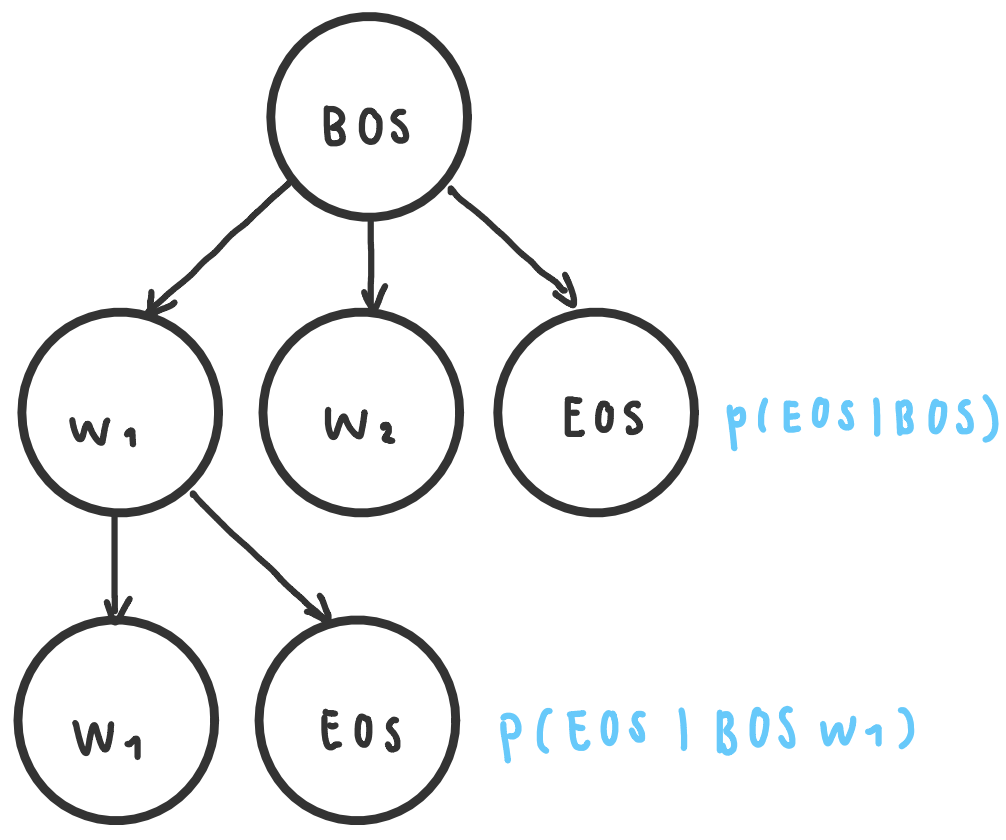
\includegraphics[height=10mm]{inhalt/images/NLP/06_language_models_1.png}
\end{multicols}
\section{N Gram Models}
\subsection*{Description}
\emph{Task} --- Predict the next word in a sequence, based on a locally normalized language model

{\color{black}\hrule height 0.001mm}

\subsection*{Formulation}
\begin{itemize}
    \item Naively, probability of a sentence: $
    p(\boldsymbol{w}) = p(w_1) \times p(w_2 \mid w_1) \times p(w_3 \mid w_1, w_2) \times \cdots \times p(w_N \mid \boldsymbol{w}_{<N}) \times p(\textrm{EOS} \mid \boldsymbol{w})
    $
    \item Challenge: Probabilities for long sequences are likely to be $0$, given the low chance of exactly such a sequence appearing in the sentence
    \item \emph{Markov assumption}: Not all words prior to the target word matter in predicting it, only the last $N-1$ words (history) are considered
    \item \emph{N-gram}:
    \begin{itemize}
        \item Sequence of $n$ words as they appear in the sentence
        \item Denoted by $w^i_j$, where $i$ and $j$ refer to words in the sentence
        \item If the vocabulary has $|\mathcal{V}|$ words, there are $|\mathcal{V}|$ (distinct) unigrams, $|\mathcal{V}|^2$ bigrams, ..., $|\mathcal{V}|^n$ N-grams, ...
        \item If the sentence (or corpus) has $M$ words, there are $M$ (potentially overlapping) unigrams, $M-1$ bigrams, ..., $M-n+1$ N-grams, ...
        \item N-gram counts are given by all distinct N-grams and how often they appear in the sentence (or corpus)
        \item N-gram probability:
        $
        p(w_t \mid w_{t-n+1}, \ldots, w_{t-1})
        $
    \end{itemize}
    \item Under Markov assumption and N-gram, probability of a sentence: 
    $
    p(\boldsymbol{w}) = \left(\prod_{t=n}^N p(w_t \mid w_{t-n+1}, \ldots, w_{t-1})\right) \times p(\textrm{EOS} \mid w_{N-n+1}, \ldots, w_N) 
    $ with appropriate BOS padding for the first $n-1$ conditional probabilities: $w_0 = w_{-1} = w_{-n+2} = \textrm{BOS}$\\
    Note: For unigrams, we don't need BOS
    \item Under this model, we have 
    \begin{itemize}
        \item $
        |\mathcal{V}|^{n-1} + |\mathcal{V}|^{n-2} + \cdots + |\mathcal{V}| + 1 = \sum_{i=0}^{n-1} |\mathcal{V}|^i
        $
        conditional probabilities for $w_t$, where 
        \begin{itemize}
            \item $|\mathcal{V}|^{n-1}$ applies if the context is fully occupied with words
            \item $1$ applies if the context only contains BOS, i.e. $w_t$ is the first token
        \end{itemize}
        \item $|\bar{\mathcal{V}}|-1$ free parameters for each conditional probability, i.e., $|\bar{\mathcal{V}}|^{n-1} \sum_{i=0}^{n-1} |\mathcal{V}|^i$ in total, where $\bar{\mathcal{V}} = \mathcal{V} \cup \{\textrm{EOS}\}$
    \end{itemize}
    \item When N-gram order is high, there is a problem of high variance (data sparsity) and when it is low, there is a problem of high bias (cannot capture long-term dependencies)
\end{itemize}

{\color{black}\hrule height 0.001mm}

\subsection*{Optimization}
Via relative frequency counts or via neural nets with log-linear model
\emph{Relative frequency counts} ---
\begin{itemize}
    \item $
    p(w_t \mid w_{t-n+1}, \ldots, w_{t-1}) = \frac{\text{count}(w_{t-n+1}, \ldots, w_{t-1}, w_t)}{\text{count}(w_{t-n+1}, \ldots, w_{t-1})}
    $\\
    Note:  In denominator, only count N-grams where the correct sequence appears in the correct position $1$ to $n-1$
    \item Corresponds to MLE estimate, if we assume each token is sampled independently from a categorical distribution over the vocabulary
    \hl{TBA}
    \item Dealing with unseen words or word combinations resulting in probability $0$:
    \begin{itemize}
        \item How likely is this?
        \begin{itemize}
            \item Given a sentence with $M+1$ words and vocabulary $\mathcal{V}$
            \item In the sentence, there are $M$ bigrams, but from the vocabulary, we can construct $|\mathcal{V}|^2$ bigrams
            \item Probability of a given bigram at index $m$ in the sentence:
            $
            \frac{1}{|\mathcal{V}|^2}
            $
            \item Thus, the probability that a given bigram does not appear at index $m$ is:
            $
            \left(1 - \frac{1}{|\mathcal{V}|^2}\right)
            $
            \item Thus, the probability that a given bigram does not appear in any of the $M$ spots is:
            $
            \left(1 - \frac{1}{|\mathcal{V}|^2}\right)^M
            $
            \item If we seek to bound the likelihood of OOV bigrams with an upper limit $\epsilon$, we have:
            $
            \epsilon \geq \left(1 - \frac{1}{|\mathcal{V}|^2}\right)^M
            $\\
            $
            \ln(\epsilon) \geq M \ln\left(1 - \frac{1}{|\mathcal{V}|^2}\right)
            $\\
            $
            \ln(\epsilon) \approx -M \frac{1}{|\mathcal{V}|^2}
            $ because $\ln(1 + \lambda) \approx \lambda$ for $\lambda \approx 0$ for $\lambda \approx 0$\\
            $
            M \geq -\ln(\epsilon) |\mathcal{V}|^2 \approx |\mathcal{V}|^2 \ln\left(\frac{1}{\epsilon}\right)
            $
        \end{itemize}
        \item Remedies:
        \begin{itemize}
            \item Consider creating an OOV category
            \item Consider \emph{additive Lidstone smoothing}:
            \begin{itemize}
                \item Smooth the PMF of the vocabulary by moving weight from seen vocabulary to unseen vocabulary by adding pseudo counts to each word:
                $
                p(w_t \mid w_{t-n+1}, \ldots, w_{t-1}) = \frac{\text{count}(w_{t-n+1}, \ldots, w_{t-1}, w_t) + \lambda}{\text{count}(w_{t-n+1}, \ldots, w_{t-1}) + |\mathcal{V}| \lambda}
                $
                \item If $\lambda = 1$, we call this \emph{Laplace smoothing}
                \item Corresponds to a MAP estimate if we assume a symmetric Dirichlet distribution with parameter $\lambda$ as our prior distribution over the weights
            \end{itemize}
            \item Consider back-off approach:
            \begin{itemize}
                \item Revert to lower-order N-grams that do not contain OOVs
                \item 
                $
                \hat{p}(w_t \mid w_{t-n+1}, \ldots, w_{t-1}) =
                \begin{cases} 
                p^*(w_t \mid w_{t-n+1}, \ldots, w_{t-1})\\ \quad \text{if } \text{count}(w_{t-n+1}, \ldots, w_{t-1}) > 0\\
                \alpha_{n-1} \ p(w_t \mid w_{t-(n-1)+1}, \ldots, w_{t-1})\\ \quad \text{otherwise}
                \end{cases}
                $
            \end{itemize}
            \item Consider interpolation: Combine estimates from different N-gram orders:
            $
            p(w_t \mid w_{t-n+1}, \ldots, w_{t-1}) = \alpha_1 p(w_t) + \alpha_2 p(w_t \mid w_{t-1}) + \ldots + \alpha_n p(w_t \mid w_{t-n+1}, \ldots, w_{t-1})
            $
        \end{itemize}
    \end{itemize}
\end{itemize}

{\color{lightgray}\hrule height 0.001mm}

\emph{Neural nets} ---
\begin{itemize}
    \item Advantage over frequency-count-based N-grams: Parameters are shared between contexts $w_{t-n+1}, \ldots, w_{t-1}$
    \item Log-linear model:
    $
    p(w_t \mid w_{t-n+1}, \ldots, w_{t-1}) = \frac{\exp(\mathbf{v}(w_t) \cdot \mathbf{h}_t)}{\sum_{w' \in \bar{\mathcal{V}}} \exp(\mathbf{v}(w') \cdot \mathbf{h}_t)}
    $
    where:
    \begin{itemize}
        \item $\mathbf{v}(w)$ are word vectors
        \item $\mathbf{h}_t$ are N-gram context vectors of the previous $n-1$ words
    \end{itemize}
    \item E.g.
    \begin{itemize}
        \item Inputs: $n-1$ words
        \item Transformation: word embedding $\boldsymbol{c}(w)$
        \item Concatenated vector of word embeddings:
        $
        \boldsymbol{c}(\boldsymbol{w}_{<3}) = [\boldsymbol{c}(w_1) \ \boldsymbol{c}(w_2) \ \boldsymbol{c}(w_3)]
        $
        \item Hidden layer:
        $
        \boldsymbol{h}_1 = f(\boldsymbol{c}(\boldsymbol{w}_{<3}))
        $
        \item Activation: Softmax:
        $
        p(w_i \mid \boldsymbol{w}_{<3}) = \frac{\exp \left( \boldsymbol{v}(w_i) \cdot \boldsymbol{h}_3 \right)}{\sum_{w' \in \bar{\mathcal{V}}} \exp \left( \boldsymbol{v}(w') \cdot \boldsymbol{h}_3 \right)}
        $
    \end{itemize}
    \item $\boldsymbol{v}(w_i), \boldsymbol{h_i}, f$, and its parameters $\theta$ are learned by maximizing log-likelihood of training dataset:
    $
    \log p(w^{(i)}) = \sum_{w^{(i)} \in D} \log \left( \prod_{t=1}^{|w^{(i)}|} p(w_t^{(i)} \mid w_{t-1}^{(i)}, \dots, w_{t-n+1}^{(i)}) \right)
    $\\
    $ = \sum_{w^{(i)} \in D} \sum_{t=1}^{|w^{(i)}|} \log \left( p(w_t^{(i)} \mid w_{t-1}^{(i)}, \dots, w_{t-n+1}^{(i)}) \right)$\\
    $ = \sum_{w^{(i)} \in D} \sum_{t=1}^{|w^{(i)}|} \boldsymbol{v}(w_t) \cdot \boldsymbol{h_t} - \log(\sum_{w' \in \bar{\mathcal{V}}} \exp ( \boldsymbol{v}(w') \cdot \boldsymbol{h_t}))$
\end{itemize}

{\color{black}\hrule height 0.001mm}

\subsection*{Evaluation}
Intrinsic evaluation: \emph{Perplexity}:
\begin{itemize}
    \item Perplexity is the normalized inverse probability of test set: Given test sequence $(w_1, \dots, w_N)$:
    $
    \text{perplexity}(w_1, \dots, w_N) = p(w_1, \dots, w_N)^{-\frac{1}{N}} 
    $
    where $N$ is the number of words in the sentence and $n$ is the N-gram order\\
    Proof:
    \begin{itemize}
        \item $
        p(w_1, \dots, w_N) = \prod_{i=1}^N p(w_i \mid w_{i-n+1}, \dots, w_{i-1})
        $
        \item Normalize by transforming to log and dividing by $N$:
        $
        \frac{\sum_{i=1}^N \log \left( p(w_i \mid \dots) \right)}{N}
        $
        \item Remove log:
        $
        \left( \prod_{i=1}^N p(w_i \mid \dots) \right)^{\frac{1}{N}}
        $
        \item Take inverse:
        $
        \frac{1}{\left( \prod_{i=1}^N p(w_i \mid \dots) \right)^{\frac{1}{N}}} = \left( \prod_{i=1}^N p(w_i \mid \dots) \right)^{-\frac{1}{N}} = \sqrt[N]{ \prod_{i=1}^N \frac{1}{p(w_i \mid w_{i-n+1}, \dots, w_{i-1})}}
        $
    \end{itemize}
\end{itemize}
\section{Part of Speech (POS) Tagging with Conditional Random Field (CRF)}
\subsection*{Description}
\emph{Task} --- 
\begin{itemize}
    \item Tag parts of speech, e.g., adverb, verb, noun, etc.
\end{itemize}

{\color{black}\hrule height 0.001mm}

\subsection*{Formulation}
\begin{itemize}
    \item Input: Sequence of words $w$ of length $N$
    \item Output: Sequence of tags $t \in T$ with $t_0 = BOS$ and $t_N = EOS$
    \item Can represented as \emph{trellis}:
    \begin{itemize}
        \item DAG, where nodes are divided into vertical slices and each slice is associated with a timestamp
        \item Each node corresponds to a distinct state
        \item Each arrow represents a transition to a new state in the next slice
    \end{itemize}
\end{itemize}

{\color{lightgray}\hrule height 0.001mm}

\emph{Point of departure} --- 
\begin{itemize}
    \item Log-linear model:
    $
    p(t \mid w) = \frac{\exp(\textrm{score}(t, w))}{Z} = \frac{\exp(\textrm{score}(t, w))}{\sum_{t'} \exp(\textrm{score}(t', w))}
    $
    \item Challenge: Naively computing $Z$ would take exponential time $\mathcal{O}(|T|^N)$
    \item Solution: Consider a scoring function that is additively decomposable over tag bigrams:
    $
    \textrm{score}(t, w) = \sum_{n=1}^N \textrm{score}(\langle t_{n-1}, t_n \rangle, w)
    $
    \item Then, we have:
    $
    p(t \mid w) = \frac{\exp( \sum_{n=1}^N \textrm{score}(\langle t_{n-1}, t_n \rangle, w) )}{\sum_{t'} \exp( \sum_{n=1}^N \textrm{score}(\langle t_{n-1}', t_n' \rangle, w) )}
    $
    \item If we take the denominator:
    \begin{itemize}
        \item $
        \sum_{t_1:t_N} \exp( \sum_{n=1}^N \dots ) = \sum_{t_1:t_N} \prod_{n=1}^N \exp(\dots) = \sum_{t_1:t_{N-1}} \sum_{t_N} \prod_{n=1}^N \exp(\dots)
        $ since last tag $t_N$ only depends on $t_{N-1}$
        \item $ = \sum_{t_1:t_{N-1}} \prod_{n=1}^{N-1} \exp(\dots) $\\$\sum_{t_N} \prod_{n=N}^{N} \exp(\textrm{score}(\langle t_{n-1}, t_n \rangle, w) ) 
        $ based on distributivity of $\otimes$ over $\oplus$
        \item $ = \sum_{t_1:t_{N-1}} \prod_{n=1}^{N-1} \exp(\dots) $\\$\sum_{t_N} \exp(\textrm{score}(\langle t_{N-1}, t_N \rangle, w) ) 
        $
        \item $ = \sum_{t_1} [ \exp(\textrm{score}(\langle t_0, t_1 \rangle, w) ) \times \sum_{t_2} [ \exp(\dots) \times \dots \times \sum_{t_N} \exp(\textrm{score}(\langle t_{N-1}, t_N \rangle, w) )]]
        $
    \end{itemize}
    \item We've moved from an exponential number of terms to a linear number of terms
    \item We go from having a score for each path in the trellis to a score for each edge
\end{itemize}

{\color{lightgray}\hrule height 0.001mm}

\emph{Backward algorithm} --- 
\begin{itemize}
    \item Algorithm for computing $Z$
    \begin{enumerate}
        \item For $t_{N-1}$ (all tags):
        $
        \beta(w, t_{N-1}) \gets \exp(\textrm{score}(\langle t_{N-1}, \textrm{EOS} \rangle, w))
        $
        \begin{itemize}
            \item Handles scores of edges incoming to EOS
            \item $\beta$ is memoized
        \end{itemize}
        \item For $n \in N-2, \dots, 1$:\\
        For $t_n \in T$ (all tags):
        $
        \beta(w, t_n) \gets \sum_{t_{n+1}} \exp(\textrm{score}(\langle t_n, t_{n+1} \rangle, w)) \times \beta(w, t_{n+1})
        $
        \begin{itemize}
            \item Handles scores over normal edges
            \item $\beta$ is memoized
        \end{itemize}
        \item 
        $
        \beta(w, t_0) \gets \sum_{t_1} \exp(\textrm{score}(\langle \textrm{BOS}, t_1 \rangle, w)) \times \beta(w, t_1)
        $
        \begin{itemize}
            \item Handles scores of edges outgoing from BOS
        \end{itemize}
        \item Return $\beta(w, t_0)$
    \end{enumerate}
    \item $\beta(w, t_n)$ are \emph{backward variables} that contain the sum of the scores of all paths starting at EOS and ending at tag $t_n$
    \item Therefore:
    $
    \textrm{denominator} = \beta(w, t_0) = \beta(w, \textrm{BOS})
    $
    \item Complexity:
    \begin{itemize}
        \item Time complexity: 
        \begin{itemize}
            \item For tag bigrams: $\mathcal{O}(N |T|^2)$, given that we compute $|T| N$ backward variables and for each of them, compute the sum over $|T|$ successor tags, repeated for the number of epochs and samples
            \item For tag trigrams: $\mathcal{O}(N |T|^3)$, repeated for the number of epochs and samples
            \item For tag N-grams of order $n$: $\mathcal{O}(N |T|^{n})$, repeated for the number of epochs and samples
        \end{itemize}
        \item Space complexity: $\mathcal{O}(N|T|)$, since we have to keep $|T| N$ backward variables in memory
    \end{itemize}
    \item Alternatively, the same can be achieved with a \emph{forward algorithm}
    \begin{itemize}
        \item Starting from BOS $t_0$ and going forward towards EOS $t_N$
        \item Instead of looking at $t_{n+1}$ we look at $t_{n-1}$
    \end{itemize}
    \item In addition to probabilities, we can compute entropy of the CRF using the expectation semiring:
    \begin{itemize}
        \item Instead of $\omega = \exp(\textrm{score}(\langle t_{n-1}, t_n \rangle, w))$, we do:
        $
        \omega = \langle \omega, -\omega \log(\omega) \rangle
        $
        \item Running the backward algorithm with these weights and in the expectation semiring, we can additionally compute unnormalized entropy $H_u = - \sum_t \exp(\textrm{score}(t, w)) \times \textrm{score}(t, w)$ in the same runtime complexity:
        \begin{itemize}
            \item We aim to show that the backward algorithm computes $\langle Z, H_u\rangle$
            \item In the base case, $\langle Z, H_u\rangle = \langle \omega, -\omega \log(\omega) \rangle$
            \item Let's call the adjusted backward variables $\beta'$, instead of $\beta$
            \item $
            \beta'(w, t_n)  \gets \bigoplus_t 
            \langle \omega(t_n, t_{n+1}), -\omega(t_n, t_{n+1}) \log(\omega(t_n, t_{n+1})) \rangle \otimes \beta'(w, t_{n+1})
            $
            \item Based on the definition of $\otimes$ under the expectation semiring, this is: $
            \beta'(w, t_n)  \gets \bigoplus_t 
            \langle Z_{n-1} \times \omega(t_n, t_{n+1}), Z_{n-1} \times -\omega(t_n, t_{n+1}) \log(\omega(t_n, t_{n+1})) + H_{u,n-1} \times \omega(t_n, t_{n+1}) \rangle = 
            \langle Z_{n-1} \times \omega(t_n, t_{n+1}), [Z_{n-1} \times -\log(\omega(t_n, t_{n+1})) + H_{u,n-1}] \times \omega(t_n, t_{n+1}) \rangle
            $
            \item Then:
            \begin{itemize}
                \item $Z_{n-1} = \sum_t \prod_{i=1}^{n-1} \omega(t_n, t_{n+1}) = \sum_t \exp(\textrm{score}(t, w))$
                \item $H_{u,n-1} = \sum_t [ \prod_{i=1}^{n-1} \omega(t_n, t_{n+1}) ][ \sum_{i=1}^{n-1} -\log(\omega(t_n, t_{n+1})) ] = -\sum_t [ \prod_{i=1}^{n-1} \omega(t_n, t_{n+1}) ][ \log(\prod_{i=1}^{n-1} \omega(t_n, t_{n+1})) ] = - \sum_t \exp(\textrm{score}(t, w)) \times \textrm{score}(t, w)$
            \end{itemize}
        \end{itemize}
        \item We can then compute the normalized entropy $H_n$:
        \begin{itemize}
            \item $H_n = -\sum_t p(t) \log(p(t))$
            \item If we substitute $p(t) = \frac{1}{Z} \exp(\textrm{score}(t, w))$, we get: $H_n = -\sum_t \frac{1}{Z} \exp(\textrm{score}(t, w)) \log(\frac{1}{Z} \exp(\textrm{score}(t, w)))$
            \item We can develop to:
            $H_n = -\sum_t \frac{1}{Z} \exp(\textrm{score}(t, w)) (\textrm{score}(t, w) - \log(Z)) = -\sum_t \frac{1}{Z} \exp(\textrm{score}(t, w))\textrm{score}(t, w) - \frac{1}{Z} \exp(\textrm{score}(t, w)) \log(Z) = \frac{1}{Z} \sum_t -[ \exp(\textrm{score}(t, w))\textrm{score}(t, w)] + \log(Z)\sum_t[\frac{1}{Z} \exp(\textrm{score}(t, w))] = \frac{1}{Z} \sum_t -[ \exp(\textrm{score}(t, w))\textrm{score}(t, w)] + \log(Z) \times 1 = Z^{-1} H_u + \log(Z)$
        \end{itemize}
    \end{itemize}
\end{itemize}

{\color{lightgray}\hrule height 0.001mm}

\emph{Viterbi algorithm} --- 
\begin{itemize}
    \item Algorithm for computing the score of the best tag sequence $t^*$ and recovering the sequence itself
    \item For this, we can ignore the denominator: $
    p(t \mid w) \propto \exp(\textrm{score}(t, w))
    $
    \begin{enumerate}
        \item For $t_{N-1}$ (all tags):
        \begin{itemize}
            \item $v(w, t_{N-1}) \gets \exp(\textrm{score}(\langle t_{N-1}, \textrm{EOS} \rangle, w))$
            \item $
            b(t_{N-1}) \gets \textrm{EOS}$ since $t_N$ can only be EOS
        \end{itemize}
        \item For $n \in N-2, \dots, 1$:\\
        For $t_n \in T$ (all tags):
        \begin{itemize}
            \item
            $
            v(w, t_n) \gets \max_{t_{n+1}} [ \exp(\textrm{score}(\langle t_n, t_{n+1} \rangle, w)) \times v(w, t_{n+1}) ]
            $ for each tag $t_n$, stores the score of the next best tag $t_{n+1}$ 
            \item $
            b(t_n) \gets argmax_{t_{n+1}} [ \exp(\textrm{score}(\langle t_n, t_{n+1} \rangle, w)) \times v(w, t_{n+1}) ]
            $ for each tag $t_n$, stores the tag $t_{n+1}$ that gave the best score
        \end{itemize}
        \item Finally:
        \begin{itemize}
            \item $
            v(w, t_0) \gets \max_{t_1} [  \exp(\textrm{score}(\langle t_0, t_1 \rangle, w)) \times v(w, t_1)]
            $
            \item $
            b(t_0) \gets argmax_{t_1} [  \exp(\textrm{score}(\langle t_0, t_1 \rangle, w)) \times v(w, t_1)]
            $
        \end{itemize}
        \item For $n = 1, \dots, N$: Recover the best sequence using backpointers, by always plugging in next $t$
        $
        t_n \gets b(t_{n-1})
        $
        \begin{itemize}
            \item $t_1 = b(\textrm{BOS})$
            \item $t_2 = b(t_1)$
            \item $...$
        \end{itemize}
        \item Return $t_{1:N}$ and $v(w, t_0)$
    \end{enumerate}
    \item $b(t_n)$ are \emph{backpointers} that point to the $t_{n+1}$ tag in $t^*$
    \item $v(w, t_n)$ are \emph{Viterbi variables} that contain the score of $t^*$ starting at EOS and ending with tag $t_n$ 
    \item Complexity:
    \begin{itemize}
        \item For backpointers: $\mathcal{O}(N)$, repeated for the number of epochs and samples
        \item For tag N-grams of order $n$: $\mathcal{O}(N |T|^n)$, repeated for the number of epochs and samples
        \item For higher-order N-grams, we apply restriction that transitions must be valid (e.g. in $t_1 \to t_2, t_3 \to t_4$ $t_2$ must equal $t3$)
    \end{itemize}
    \item Alternatively, the same can be achieved with a \emph{forward Viterbi algorithm}
    \begin{itemize}
        \item Starting from BOS $t_0$ and going forward towards EOS $t_N$
        \item Instead of looking at $t_{n+1}$ we look at $t_{n-1}$
        \item Backpointers point to the $t_{n-1}$ tag in $t^*$, i.e. $t_{n-1} \gets b(t_n)$, starting with $t_{N-1} \gets b(\textrm{EOS}), t_{N-2} \gets b(t_{N-1}),...$
    \end{itemize}
\end{itemize}

{\color{lightgray}\hrule height 0.001mm}

\emph{Dijkstra’s algorithm} --- 
\begin{itemize}
    \item Alternative to the Viterbi algorithm:
    \begin{itemize}
        \item First complete tagging popped from the queue is the score for the best tagging, same as what Viterbi computes
        \item If we keep running Dijkstra’s algorithm until queue is empty (i.e. if we don't leverage early stopping), Dijkstra’s algorithm computes the same values $\gamma$ as Viterbi
    \end{itemize}
    \item Runs over time step - tag nodes $\langle n, t \rangle$
    \item Uses \emph{Popped} to keep track of nodes $\langle n, t \rangle$ that have been processed
    \item Uses \emph{PriorityQueue}:
    \begin{itemize}
        \item Contains node : score pairs $\langle\langle n, t \rangle, \textrm{score}\rangle$
        \item Returns pair with highest score first, regardless of time step or tag, thus, does not necessarily progress over nodes sequentially by time step, but progresses over nodes by descending score
        \item If there is no score yet for key $\langle n, t \rangle$ in queue, it's inserted
        \item If there is already a score for key $\langle n, t \rangle$ in queue, the higher score is retained: $\max_{\textrm{score}} \textrm{score}$
    \end{itemize}
    \item Uses table $\gamma$ to store the best score for each node $\langle n, t \rangle$: $\gamma[n, t] = \textrm{score}$
    \item Algorithm:
    \begin{enumerate}
        \item Initialize:
        \begin{itemize}
            \item Popped $\gets \{ \}$
            \item Queue $\gets$ $\textrm{Priority Queue}()$
            \item $\gamma \gets -\infty$
        \end{itemize}
        \item Push $\langle\langle 0, \textrm{BOS} \rangle, 0\rangle$ to queue
        \item While $|\textrm{queue}| > 0$:
        \begin{enumerate}
            \item Pop $\langle \langle n, t \rangle, \textrm{score} \rangle$ from queue, add $\langle \langle n, t \rangle, \textrm{score} \rangle$ to popped, 
            $
            \gamma[n, t] \gets \textrm{score}
            $
            \item If $n = |w|$ or stop early: Return score    
            \item If $n < |w|$:\\
            For $t' \in T$:\\
            If $\langle n+1, t' \rangle$ is not in popped:
            Push
            $
            \langle \langle n+1, t' \rangle, \textrm{score}(t, t', w) + \gamma[n, t] \rangle
            $
            to queue
        \end{enumerate}
        \item Return $\gamma$
    \end{enumerate}
    \item Complexity:
    \begin{itemize}
        \item For tag bigrams: $\mathcal{O}(N |T|^2 \log(N |T|))$, where $\log(N |T|)$ stems from push and update operations on the queue
        \item Dijkstra's is generally slower than Viterbi, unless we leverage early stopping conditions
    \end{itemize}
    \item Dijkstra's as an alternative to Viterbi requires a semiring which guarantees:
    \begin{itemize}
        \item Idempotence of $\oplus$ such that algorithm progresses towards the optimal path without revisiting nodes
        \item Commutative and associative property of $\oplus$ such that score accumulation always yields same result, even if the nodes are processed in a different order
        \item $\mathbb{R}_{\leq0}$ since scores are log-probabilities, which are always non-positive, since probabilities are in $[0,1]$
    \end{itemize}
    \item Dijkstra's could also be used as an alternative to the backward algorithm with a different semiring
    \hl{TBA}
\end{itemize}

{\color{lightgray}\hrule height 0.001mm}

\emph{Generalized algorithm} --- 
\begin{itemize}
    \item A more general formulation of backward, Viterbi, and Dijkstra's algorithms using semirings
    \item Backward algorithm: Uses inside semiring
    \item Viterbi algorithm: Uses Viterbi semiring
    \item Challenge with this original formulation: Multiplying probabilities for long sequences may cause numbers to go to $0$, leading to numerical underflow
    \item Solution: Revert to log-sum-exp semiring (backward algorithm) resp. arctic semiring (Viterbi algorithm). Note: The log-sum-exp semiring returns the log normalizer ($log(Z)$) instead of the normalizer ($Z$)
    \item Dijkstra's algorithm: Uses arctic semiring
\end{itemize}

{\color{lightgray}\hrule height 0.001mm}

\emph{Scoring functions} --- 
\begin{itemize}
    \item So far, we only imposed the requirement that the scoring function is additively decomposable, but we have not specified it further
    \item \emph{Hidden Markov Model}:
    $
    \textrm{score}(\langle t_{n-1}, t_n \rangle,w) = \textrm{transition}(t_{n-1}, t_n) + \textrm{emission}(t_n, w_n) =
    $ transition probability (tag-tag pairs) $+$ emission probability (word-tag pairs) except for $t_N =$ EOS, where we have no emission probability: $
    \textrm{score}(\langle t_{N-1}, t_N \rangle,w) = \textrm{transition}(t_{N-1}, t_N) + 0
    $
    \item A more complex example of scoring functions is a neural network with inputs $\langle t_{n-1}, t_n \rangle$ and $w$
    \item Runtime complexity of scoring function for N-grams of order $n$ and output vector dimensionality of feature function $d$ is $\mathcal{O}(d |T|^n)$, repeated for the number of epochs and samples 
    \item E.g. for the sentence 'The girl drinks':
    \begin{itemize}
        \item $\textrm{score}(w = \textrm{The girl drinks}, t = \langle D, N, V \rangle) = \sum_{n=1}^{N} \textrm{score}(\langle t_{n-1}, t_n \rangle, w)$
        \item $= \textrm{score}(\langle \textrm{BOS}, D \rangle, w) + \textrm{score}(\langle D, N \rangle, w) + \textrm{score}(\langle N, V \rangle, w) + \textrm{score}(\langle V, \textrm{EOS} \rangle, w)$
        \item Combination of emission and transition features: $(w_1 = \textrm{The}, y_1 = D) + (y_1 = D, y_0 = \textrm{BOS}) + (w_2 = \textrm{girl}, y_2 = N) + (y_2 = N, y_1 = D) + (w_3 = \textrm{drinks}, y_3 = V) + (y_3 = V, y_2 = N) + (y_4 = \textrm{EOS}, y_3 = V)$
    \end{itemize}
\end{itemize}

{\color{black}\hrule height 0.001mm}

\subsection*{Optimization}
\emph{Objective function} --- 
\begin{itemize}
    \item Assume we have a dataset of $K$ data points $( w^{(i)}, t^{(i)} )$
    \item Log likelihood:
    $
    \sum_{k=1}^K \log(p(t^{(k)} \mid w^{(k)})) = \sum_{k=1}^K \log ( \frac{\exp(\textrm{score}(t^{(k)}, w^{(k)}))}{\sum_{t'} \exp(\textrm{score}(t', w^{(k)}))} ) = \sum_{k=1}^K [ \textrm{score}(t^{(k)}, w^{(k)}) - \log \sum_{t'} \exp(\textrm{score}(t', w^{(k)})) ]
    $
    \item Risk of overflow since sum makes things big and log makes things small
    \item If we want to use a temperature parameter $T$, we have:
    $
    \sum_{k=1}^K \log(p(t^{(k)} \mid w^{(k)})) = \sum_{k=1}^K \log ( \frac{\exp(\textrm{score}(t^{(k)}, w^{(k)})/ T)}{\sum_{t'} \exp(\textrm{score}(t', w^{(k)})/ T)} ) = \sum_{k=1}^K [ \frac{\textrm{score}(t^{(k)}, w^{(k)})}{T} - \log \sum_{t'} \exp(\frac{\textrm{score}(t', w^{(k)})}{T}) ]
    $
    \item As $T \to 0$:
    \begin{itemize}
        \item The numerator $\exp(\textrm{score}(t^{(k)}, w^{(k)})/ T)$ becomes very large for high score sequences and very small for low score sequences
        \item The denominator $\sum_{t'} \exp(\textrm{score}(t', w^{(k)})/ T)$ becomes dominated by the sequence with the highest score
        \item Then, the likelihood approaches $1$ for the sequence with the highest score and $0$ for all other sequences
    \end{itemize}
\end{itemize}

\begin{multicols}{2}
\textit{1) Trellis}\\
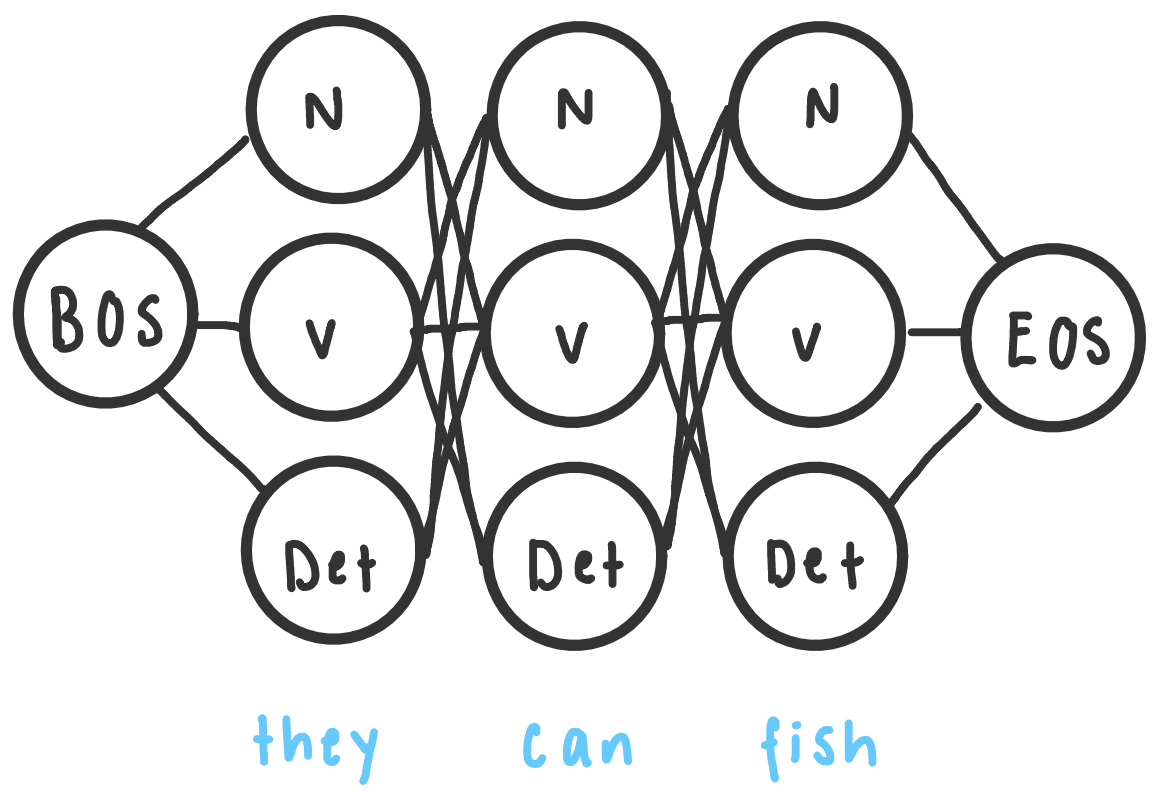
\includegraphics[height=10mm]{inhalt/images/NLP/06_pos_1.png}
\\\\
\textit{2) Backward algorithm}\\
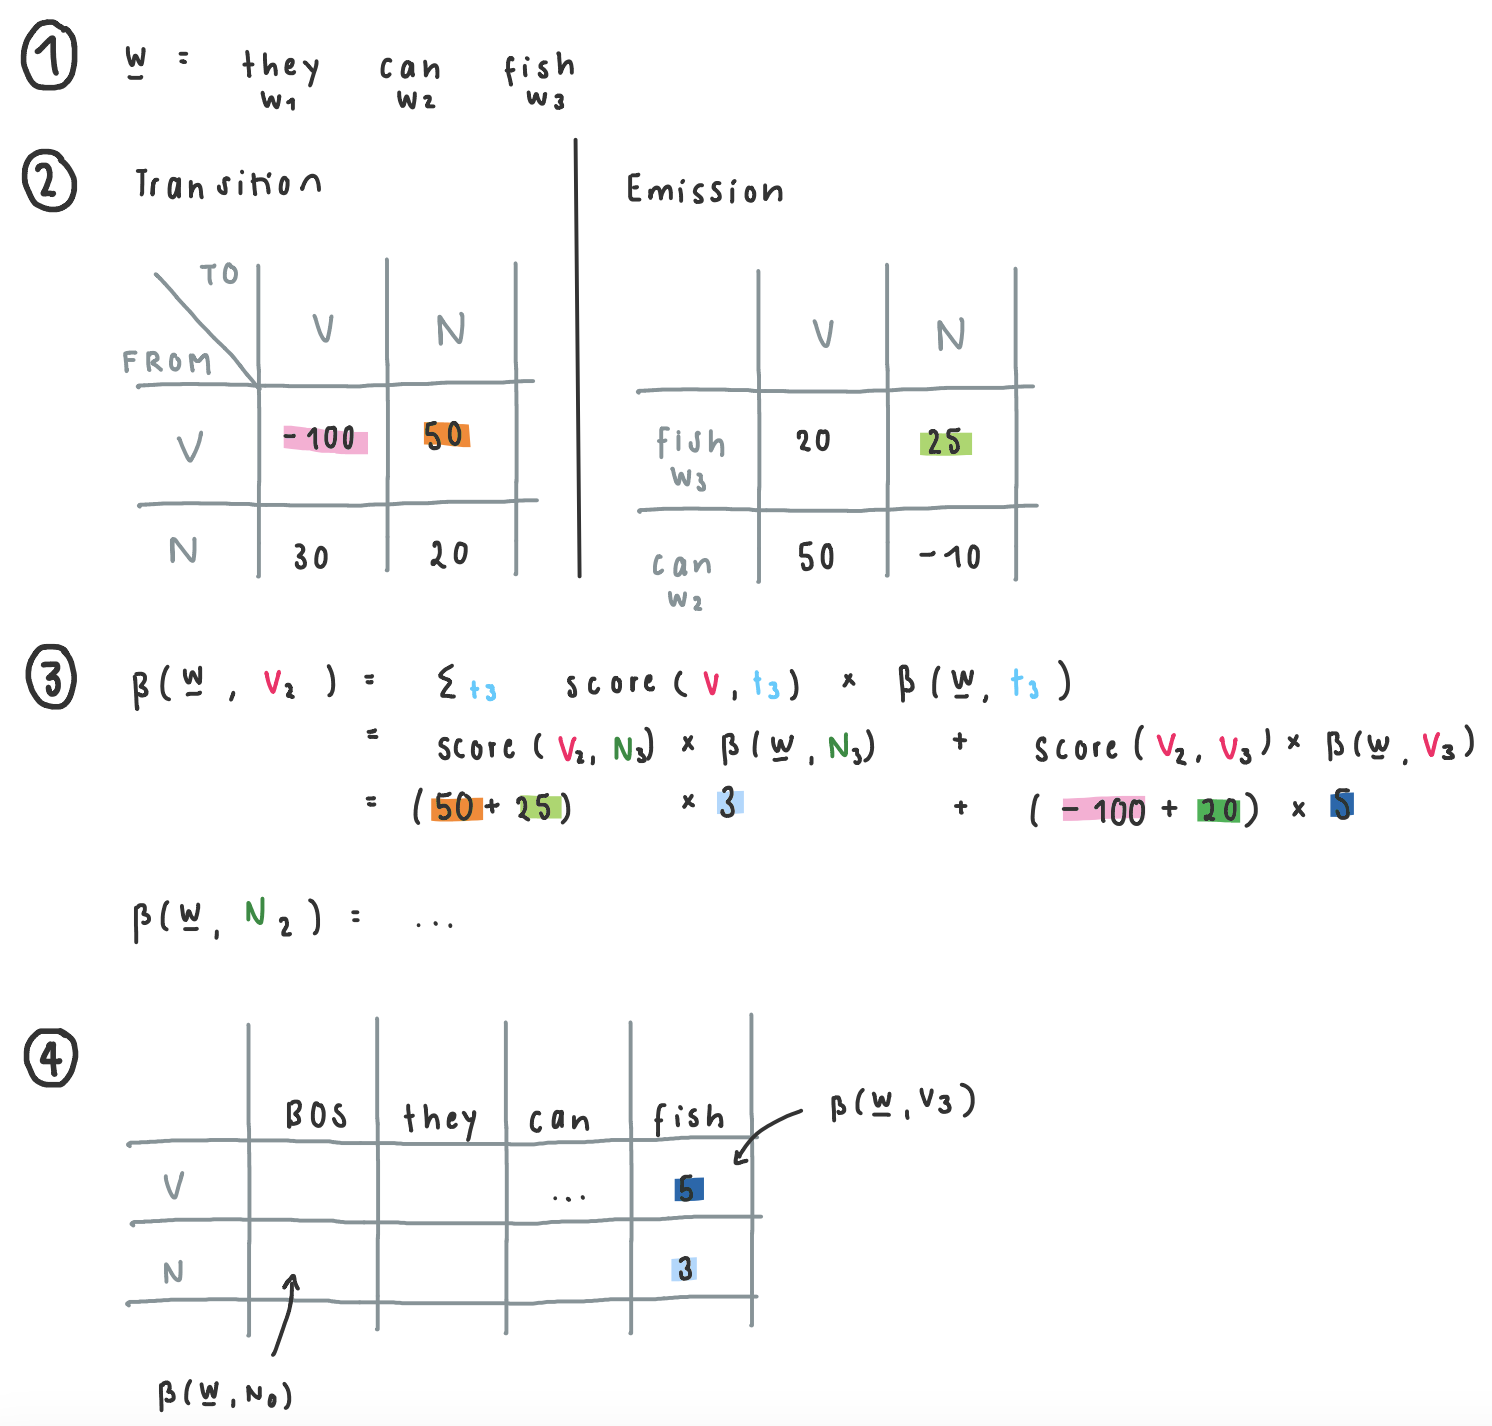
\includegraphics[height=25mm]{inhalt/images/NLP/06_pos_2.png}
\end{multicols}
\section{Syntax | Syntactic Parsing}
\subsection*{Description}
\emph{Task} --- Assign syntactic structure, i.e., parse tree, to a sentence by breaking it down into a hierarchy of constituents that is grammatically correct (similar to dependency parsing)

{\color{lightgray}\hrule height 0.001mm}

\emph{Terminology} ---
\begin{itemize}
    \item \emph{Constituent}: Sequence of words that function as a coherent unit resp. nodes in tree
    \begin{itemize}
        \item \emph{Terminals}: Words
        \item \emph{Non-terminals}: Abstractions over words, e.g., noun phrases
    \end{itemize}
    \item \emph{Grammar}: Set of rules (productions), according to which sentences (strings) can be formed from a vocabulary
    \begin{itemize}
        \item \emph{Context-free grammar (CFG)}: Grammar where rules are applied regardless of context
    \end{itemize}
    \item \emph{Parse tree}: 
    \begin{itemize}
        \item Represents both syntactic structure of a string and its derivation under grammar
        \item Can be considered a bag of production rules and a multiset (i.e., set with repeats)
    \end{itemize}
\end{itemize}

{\color{black}\hrule height 0.001mm}

\subsection*{Context-Free Parsing}
\emph{Context-free grammar $(\mathcal{N}, \mathcal{S}, \Sigma, \mathcal{R})$} ---
\begin{itemize}
    \item Finite set of non-terminal symbols $\mathcal{N} = \{N_1, N_2, \dots\}$
    \item Distinguished start non-terminal $\mathcal{S}$
    \item Alphabet of terminal symbols $\Sigma = \{a_1, a_2, \dots\}$
    \item Set of production rules of the form $N \to \alpha$, where $N$ is non-terminal and $\alpha \in (\mathcal{N} \cup \Sigma)^*$, i.e. $\alpha$ is either terminal or non-terminal
    \item Examples:
    \begin{itemize}
        \item Language $\{a^i b^j c^k \mid i, j, k \geq 0, i + j = k\}$ is generated by:
        $
        \mathcal{S} \to a \mathcal{S} c \mid W \mid \varepsilon$
        $W \to bW \mid \varepsilon
        $
        \item Language $\{a^i b^j c^k \mid i, j, k \geq 0, i + k = j\}$ is generated by:
        $
        \mathcal{S} \to KW$
        $K \to aKb \mid \varepsilon$
        $W \to bWc \mid \varepsilon$
        \item Language $\{w \in \{a, b\}^* \mid w \textrm{ contains min. }3 a\}$ is generated by:
        $
        \mathcal{S} \to WaW aW aW$
        $W \to aW \mid ab \mid \varepsilon
        $
    \end{itemize}
\end{itemize}

{\color{lightgray}\hrule height 0.001mm}

\emph{Pumping lemma} ---
\begin{itemize}
    \item In any CFG, long enough strings have some kind of repeating structure
    \item Then, there exists a $k$ such that a string $s$ with $|s| > k$ can be written as $s = u x y z v$, where:
    \begin{itemize}
        \item $u, y, v$ are "fixed" parts, whereas $x$ and $z$ are "pumpable" parts
        \item $u x^n y z^n v$ is also in the CFG
        \item $x$ and $z$ are not empty
        \item $|x y z| < k$
    \end{itemize}\\
    Proof:
    \begin{itemize}
        \item Consider a parse tree with height $|\mathcal{V}| + 1 = N$. This tree uses all symbols in $|\mathcal{V}|$. Thus, any tree with height $> N$ must include some repetition of symbols
        \item Let $k >$ length of any string yielded by a tree with max height $N$
        \item If $|s| \geq k$, then $s$ must be yielded by a tree with height $> N$, meaning $s$ must include repetition of at least one symbol $A$
        \item From this, properties follow:
        \begin{itemize}
            \item If $T$ is the entire parse tree, $T_A$ is the parse tree with root upper $A$, and $T_{AA}$ is the parse tree with root lower $A$
            \item $T_A$ has height $\leq N$, i.e., $|xyz| < K$
            \item If $x$ and $z$ are empty (i.e., we replace $T_A$ with $T_{AA}$), we have a smaller tree that yields $s$, which is a contradiction
            \item We can extend the proof to any $n$
        \end{itemize}
    \end{itemize}
    \item Pumping lemma shows that languages that require strict equality between counts of $3+$ symbols cannot be generated by a CFG
\end{itemize}
\hl{INSERT IMAGE 1}

{\color{lightgray}\hrule height 0.001mm}

\emph{Span} ---
\begin{itemize}
    \item Contiguous segment of a sentence from word $w_i$ to $w_{j-1}$: $[i, j]$
    \item Span is admissible if it is possible to construct a parse tree, which covers exactly that span and is a valid constituent according to the grammar, i.e., there exists a non-terminal $X$ such that $X \to w[i:j]$
    \item For string of length $M$, we have:
    $
    [M, M+1)
    $ for span size $= 1$
    $
    [1, M+1)
    $ for span size $= M$
    More generally:
    $
    [M - \textrm{span size} + 1, M + 1)
    $
\end{itemize}

{\color{lightgray}\hrule height 0.001mm}

\emph{Chomsky Normal Form (CNF)} ---
\begin{itemize}
    \item CFG, where production rules follow specific structure:
    \begin{itemize}
        \item $N_1 \to N_2 N_3$ are non-terminal productions
        \item $N_- \to a_-$ are terminal productions
    \end{itemize}
    \item Prohibits cyclic rules
\end{itemize}

{\color{lightgray}\hrule height 0.001mm}

\emph{Probabilistic CFGs} ---
Motivation:
\begin{itemize}
    \item Often, multiple syntactic structures are grammatically admissible, i.e., the string is ambiguous
    \item This is the case when a non-terminal can be produced by two rules
\end{itemize}
Probabilistic CFGs $(\mathcal{N}, \mathcal{S}, \Sigma, \mathcal{R}, \mathcal{P})$:
\begin{itemize}
    \item Additionally define a set of probabilities $\mathcal{P}$ for each production rule
    \item Probabilities are locally normalized over each transition:
    $
    \sum_{k} p(N \to \alpha_k) = 1
    $
    where $N \to \alpha_1, \dots, N \to \alpha_k$ are expansions of node $N$
    \item For example:
    $
    \text{NP} \to \text{VP} (p = 0.6) \mid \text{Adj} (p = 0.4)
    $
    with total $p = 1$
    \item Then, the probability of a parse tree is the multiplication of the probabilities of the rules used to create the tree:
    $
    p(t) = \prod_{r \in t} p(r) = p(S \to S_1 S_2)^{M-1} \times p(S \to X)^M \times p(X \to Y)^M
    $
    where:
    \begin{itemize}
        \item $p(S \to S_1 S_2)^{M-1}$: repeats the rule $S \to SS$ $M-1$ times to obtain $M$ starting nodes
        \item $t$: tree
        \item $r$: rule
        \item $S$: start non-terminal
        \item $X$: non-terminal
        \item $Y$: terminal
        \item $M$: sentence length
    \end{itemize}
\end{itemize}

{\color{lightgray}\hrule height 0.001mm}

\emph{Weighted CFGs} ---
\begin{itemize}
    \item A more general formulation of PCFGs
    \item Probabilities are globally normalized over all possible parse trees
    \item Probability of a parse tree:
    $
    p(t) = \frac{1}{Z} \prod_{r \in t} \exp(\textrm{score}(r))
    $
    where:
    $
    Z = \sum_{t' \in T} \prod_{r \in t'} \exp(\textrm{score}(r))
    $
    \item Challenge: The denominator $Z(s)$ is infinitely large, potentially even larger than $\Sigma^*$ for ambiguous strings
    \item Initial solution: Probability of a parse tree, conditioned on string $s$:
    $
    p(t \mid s) = \frac{1}{Z(s)} \prod_{r \in t} \exp(\textrm{score}(r))
    $
    where:
    $
    Z = \sum_{t' \in T(s)} \prod_{r \in t'} \exp(\textrm{score}(r))
    $ 
    where $T(s)$ is set of trees that yield $s$
    \item Challenge: The denominator $Z(s)$ is still potentially infinitely large due to cyclic rules
    \item Final solution: Revert to CNF. Then, $|T(s)|$ for a string of length $M$ is the number of rooted binary trees, which is the Catalan number $C_{M-1}$
    \item With CNF, probability of a parse tree:
    $p(t \mid s) = \frac{1}{Z(s)} \prod_{N_i \to N_j N_k, \in t} \exp(\textrm{score}(N_i \to N_j N_k)) \times \prod_{N_l \to a, \in t} \exp(\textrm{score}(N_l \to a))$ where
    \begin{itemize}
        \item $Z(s) = \sum_{t' \in T(s)} \prod_{N_i \to N_j N_k, \in t'} \exp(\textrm{score}(N_i \to N_j N_k)) \times \prod_{N_l \to a, \in t'} \exp(\textrm{score}(N_l \to a))$
        \item Non-terminal productions: $\prod_{N_i \to N_j N_k, \in t} \exp(\textrm{score}(N_i \to N_j N_k))$
        \item Terminal productions: $\prod_{N_l \to a, \in t} \exp(\textrm{score}(N_l \to a))$
    \end{itemize}
    \item Can be trained via MLE with backpropagation and gradient descent
\end{itemize}

{\color{lightgray}\hrule height 0.001mm}

\emph{Cocke-Kasami-Younger (CKY) Algorithm} ---
\hl{INSERT IMAGE 2}
\begin{itemize}
    \item Tasks:
    \begin{itemize}
        \item Solve the \emph{recognition problem}: Determine if a given string is admissible by the grammar
        \item Compute the normalizing constant $Z$
        \item Find one or $k$ best syntactic parses
    \end{itemize}
    \item Requires grammar in CNF
    \item Algorithm to compute normalizing constant $Z$:
    \begin{itemize}
        \item Uses real semiring with $+, \times,0,1$
        \item Alternatively, uses log-sum-exp semiring with $\log_+, +, -\infty, 0$ where 
        $
        \log_+(x, y) = \log(e^x + e^y),
        $
    \end{itemize}
    \begin{enumerate}
        \item $N \gets |s|$
        $\textrm{chart} \gets 0$
        \item For $n = 1, \dots, N$:\\
        For $X \to S_n$ (handles single word tokens) where $X \equiv N_l$, $S_n \equiv a$ in weighted CGF:
        \begin{enumerate}
            \item If real semiring: $
            \textrm{Chart}[n, n+1, X] \mathrel{+}= \exp(\textrm{score}(X \to S_n))
            $ (weight assigned to the given rule)
            \item If log-sum-exp semiring: $
            \textrm{Chart}[n, n+1, X] = \log_+( \textrm{Chart}[n, n+1, X])
            $
        \end{enumerate}
        \item For span $= 2, \dots, N$:\\
        For $i = 1, \dots, N-\textrm{span}+1$ ($i$: beginning of span):\\
        $k \gets i + \textrm{span} - 1$ ($k$: end of span)\\
        For $j = i+1, \dots, k-1$ ($j$: breaking point of span):\\
        For $X \to Y Z$ where $X \equiv N_i$, $Y \equiv N_j$, $Z \equiv N_k$ in weighted CGF:
        \begin{enumerate}
            \item If real semiring: $\textrm{Chart}[i, k, X] \mathrel{+}= \exp(\textrm{score}(X \to Y Z)) \times \textrm{Chart}[i, j, Y] \times \textrm{Chart}[j, k, Z]$ where
            \begin{itemize}
                \item Score is weight assigned to the given rule
                \item Chart entries contains normalization factors for subtrees at $i,j$ resp. $j,k$
            \end{itemize}
            \item If log-sum-exp semiring: $
            \textrm{Chart}[i, k, X] = \log_+( \textrm{Chart}[i, k, X])
            $
        \end{enumerate}
        \item Return $\textrm{Chart}[1, N+1, \mathcal{S}]$, which contains the normalization constant
    \end{enumerate}
    \item Complexity:
    \begin{itemize}
        \item Runtime complexity: $\mathcal{O}(N^3 |\mathcal{R}|)$
        \item Space complexity: $\mathcal{O}(N^2 |\mathcal{R}|)$
        \item If, for each span length, there is only one admissible span and we know $i$ (beginning) and $j$ (breaking point), we can omit looping over $i$ and $j$ and set:
        $i = N - \textrm{span size} + 1$\\
        $j = i + 1$
        \item Then, runtime complexity: $\mathcal{O}(N |\mathcal{R}|)$
    \end{itemize}
    \item Algorithm to find best parse: Run above algorithm with $\max, +$ semiring
    \item Algorithm to find whether string is admissible by grammar: Run above algorithm with Boolean semiring
\end{itemize}
\section{Syntax | Dependency Parsing}
\subsection*{Description}
\emph{Task} --- 
Assign syntactic structure to a string by breaking it down into a hierarchy of dependencies (similar to syntactic parsing)

{\color{black}\hrule height 0.001mm}

\subsection*{Formulation}
\begin{itemize}
    \item String $w$
    \item \emph{Spanning tree}: 
    \begin{itemize}
        \item Connects $N$ nodes via $N-1$ edges
        \item Contains no cycles
        \item Number of nodes can be given by number of words in sentence $|w| = N$ or, if there are dependency parsing rules available, by number of items in the dependency rules (counting each item before and after the $\to$ separately, excl. the root, e.g. $\textrm{ROOT}\to\textrm{foo}, \textrm{foo}\to\textrm{bar},\textrm{foo}\to\textrm{baz}$ has 5 nodes)
    \end{itemize}
    \item For dependency parsing, we also require:
    \begin{itemize}
        \item The tree has exactly one root node, with only one outgoing edge
        \item All non-root nodes have exactly one incoming edge
        \item Edges are directed
        \item Edges are labeled
    \end{itemize}
    \item We can turn syntactic parsing into dependency parsing based on rules:
    \begin{itemize}
        \item Head of a production rule in syntactic parsing is the head of the dependency relation in dependency parsing
        \item Then, an arrow goes from the head to the sibling
        \item Then, weight for the given production rule in syntactic parsing is the weight assigned to the head-sibling dependency in dependency parsing
        \item E.g. in $NP \to Adj N$, $N$ is the head, so there is an arrow from $N$ to $Adj$
    \end{itemize}
    \item Types of dependency trees:
    \begin{itemize}
        \item \emph{Projective trees}:
        \begin{itemize}
            \item No crossing arcs
            \item Closely related to constituents (syntactic parsing)
            \item Note: In syntactic parsing, dependency relationships are always nested within constituents, meaning that syntactic parsing trees are always projective
        \end{itemize}
        \item \emph{Non-projective trees}:
        \begin{itemize}
            \item Crossing arcs
            \item In focus in the following
        \end{itemize}
    \end{itemize}
\end{itemize}

{\color{lightgray}\hrule height 0.001mm}

\emph{Probability of spanning tree} ---
\begin{itemize}
    \item 
    $
    p(t \mid w) = \frac{\exp(\textrm{score}(t, w))}{Z} = \frac{\exp(\textrm{score}(t, w))}{\sum_{t'} \exp(\textrm{score}(t', w))}
    $
    \item Challenge: Naively:
    \begin{itemize}
        \item There are $N^N$ undirected trees in graph if we don't impose a spanning tree structure and every node can depend on any other node, including itself, meaning it takes $\mathcal{O}(N^N)$ time to compute $Z$ 
        \item \emph{Cayley's formula}: There are $N^{N-2}$ undirected trees in graph if we impose a spanning tree structure constraint, meaning it takes $\mathcal{O}(N^{N-2})$ time to compute $Z$
        \item There are $(N-1)^{N-2}$ undirected trees in graph if we also impose the constraint that there is exactly one root node, meaning it takes  $\mathcal{O}((N-1)^{N-2})$ time to compute $Z$
    \end{itemize}
    \item Solution: 
    \begin{itemize}
        \item \emph{Edge factored assumption}:
        \begin{itemize}
            \item $
            p(t \mid w) = \frac{\prod_{(i \to j) \in t} \exp(\textrm{score}(i, j, w)) \exp(\textrm{score}(r, w))}{Z} = \frac{\prod_{(i \to j) \in t} \exp(\textrm{score}(i, j, w)) \exp(\textrm{score}(r, w))}{\sum_{t'} \prod_{(i \to j) \in t'} \exp(\textrm{score}(i, j, w)) \exp(\textrm{score}(r, w))}
            $ where $(i \to j)$ is an edge in the tree, $r$ is the root 
            \item Sp, in the denominator, we sum over the number of trees ($N^{N-2}$), and in the score, we sum over the number of edges ($N-1$)
            \item In edge factored assumption, scoring function $\textrm{score}(t, w)$ can only consider features that only depend on the edge $(i \to j)$ (e.g. length $|i-j|$) or do not depend on the edges at all (e.g. length of $\boldsymbol{w}$, tags of $w_i, w_j$, embeddings of $w_i, w_j, \boldsymbol{w}$, identity of words $w_i, w_j$), but not features that depend on other edges (e.g. higher-order dependency parsing, assigned root)
        \end{itemize}
        \item \emph{Kirchhoff's Matrix-Tree Theorem}: Method for counting the number of undirected spanning trees in $\mathcal{O}(N^3)$ time
        \item \emph{Tutte's Matrix-Tree Theorem}: Generalizes Kirchhoff's Matrix-Tree Theorem to directed spanning trees:
        \begin{itemize}
            \item Take adjacency matrix and root vector:
            \begin{itemize}
                \item \emph{Adjacency matrix}: One entry for each node $i$ to node $j$, if they were connected via an edge $i \to j$
                $
                A_{ij} = \exp(\textrm{score}(i, j, w))
                $
                with 0 on diagonal and not-null on off-diagonal
                \item \emph{Root vector}: One entry for each node $j$, if it were the root node
                $
                \rho_j = \exp(\textrm{score}(j, w))
                $
            \end{itemize}
            \item Construct \emph{Laplacian matrix}:
            Not accounting for constraint that there is only one root node:
            $L_{ij} =
            \begin{cases}
                -A_{ij} & \text{if } i \neq j \\
                \rho_j + \sum_{k \neq i} A_{kj} & \text{otherwise}
            \end{cases}$\\
            Accounting for constraint that there is only one root node:
            $L_{ij} =
            \begin{cases}
                \rho_j & \text{if } i = 1 \\
                \sum_{i'=1,i' \neq j}^n A_{i'j} & \text{if } i = j \\
                -A_{ij} & \text{otherwise}
            \end{cases}$
            i.e. 
            $\begin{cases}
                \text{- first row of L contains root scores} \\
                \text{- diagonal of L (except } L_{1,1} \text{) contains}\\
                \text{sum within each column of } A \text{ (except } A_{i,i} \text{)}\\
                \text{- off-diagonal of L (except first row) contains}\\ \text{elements of A multiplied with $-1$ }
            \end{cases}$
            \item According to matrix tree theorem: $|L| = \det(L) = Z =$ number of trees in graph
            \item According to Cayley's formula: number of undirected spanning trees in graph = $N^{N-2}$
        \end{itemize}
        \item Then, we can compute $Z$ under the edge factored assumption in $\mathcal{O}(N^3)$
    \end{itemize}
\end{itemize}

{\color{black}\hrule height 0.001mm}

\subsection*{Optimization}
Construct tree:
\begin{itemize}
    \item $N$ nodes plus 1 extra root node
    \item $N-1$ edges, of which $1$ edge is fixed (root) 
    \item Number of directed spanning trees: $N^{(N-1)}$
    \item Number of directed spanning trees, including labeling of edges: $N^{(N-1)} \times x$ where $x$ is given by the number of the destination nodes (e.g. $N$) raised to the power of the number of edges that can vary (e.g. $N-1-1 = N-2$), i.e. $N^{(N-2)}$
\end{itemize}

Decode tree:
\begin{itemize}
    \item Challenge: To perform decoding, greedy \emph{Kruskal's algorithm} does not work, since this selects the highest-scoring edge at each steps, which may be suboptimal in the directed case
    \item Solution: \emph{Chu-Liu/Edmonds algorithm}
\end{itemize}

\emph{Chu-Liu/Edmonds algorithm}:
\begin{itemize}
    \item Algorithm:
    \begin{enumerate}
        \item Greedy algorithm selects best incoming edge for each node, except the root
        \item This can cause cycles, which we need to contract:
        \begin{itemize}
            \item Cycle treated as one node
            \item Edges between nodes in the cycle are \textcolor{gray}{dead}
            \item Edges between nodes fully outside the cycle are \textcolor{teal}{external}
            \item Edges exiting the cycle are \textcolor{blue}{exits}
            \item Edges entering the cycle are \textcolor{magenta}{enters}
        \end{itemize}
        \item Break cycle: For each enter edge, break cycle by removing edges that are also incoming at the node where the enter edge is incoming
        \item Re-weight: To enter edge, add weights of remaining edges that are strictly on (not in) the cycle
        \item Now, greedy algorithm selects tree without cycles
        \item Then, we can re-expand: Pick edge of highest-scoring enter edge in contracted form, pick edges that were used to re-weight when breaking cycle on that enter edge
    \end{enumerate}
    \item Without root constraint: Can be run in $\mathcal{O}(N^2)$ time
    \item With root constraint:
    \begin{itemize}
        \item Naively: Run above algorithm $N$ times, fixing each edge as the only one emanating from the root, adds factor $N$ to runtime
        \item Solution: Adjusted algorithm
    \end{itemize}
    \item Adjusted algorithm:
    \begin{enumerate}
        \item Run steps $1-4$ (contract cycle, break cycle, re-weight edges) as above
        \item If there are multiple edges emanating from the root: For each root edge, calculate cost of deleting this edge: Cost = Weight of root edge - weight of next-best incoming edge to target node (treating any cycles as single nodes)
        \item Preliminarily remove edge with lowest cost, but keep target node intact
        \item Preliminarily repeat step $2$ (calculate root edge cost, remove lowest-cost root edge) here as needed
        \item Re-run greedy algorithm in contracted form
        \item If this leads to a cycle: Undo removal of edge with lowest cost, contract (treating any cycles as single nodes), then re-expand\\
        Otherwise: Re-expand
    \end{enumerate}
\end{itemize}

{\color{black}\hrule height 0.001mm}

\subsection*{Other}
\emph{First vs. second-order dependency parsing} ---
\begin{itemize}
    \item Above, we have considered first-order dependency parses only, but this can be extended
    \item \emph{Grandparent} $g$, \emph{parent} $h$, \emph{sibling} $s$, \emph{trailing sibling} $t$, \emph{modifier} $m$, where root can be a grandparent or parent
    \begin{itemize}
        \item \emph{First-order dependency parsing}:
        \begin{itemize}
            \item Considers only direct parent-modifier relationships
            \item $h \rightarrow m$
        \end{itemize}
        \item \emph{Second-order dependency parsing}: Extends to include:
        \begin{itemize}
            \item Parent-sibling relationships: $h \rightarrow s; h \rightarrow m$
            \item Grandparent-parent-modifier relationships: $g \rightarrow h \rightarrow m$
        \end{itemize}
        \item \emph{Third-order dependency parsing}: Further extends to include:
        \begin{itemize}
            \item Grandparent-parent relationships: $g \rightarrow h; h \rightarrow s; h \rightarrow m$
            \item Parent-trailing sibling relationships: $h \rightarrow t; h \rightarrow s; h \rightarrow m$
        \end{itemize}
    \end{itemize}
    \item Edge scores:
    \begin{itemize}
        \item $k$ is grandparent, $i$ is parent, $j$ is modifier, $s$ is sibling
        \item Probability of spanning tree: $
        p(t \mid w) = \frac{1}{Z} \exp(\textrm{score}(t, w))
        $ 
        \item First-order dependency parsing: Score given by:
        $\Psi(\boldsymbol{y}, \boldsymbol{w}; \theta) =
        \sum_{i \xrightarrow{r} j \in \boldsymbol{y}} \left[ \psi_{\text{parent}}(i \xrightarrow{r} j, \boldsymbol{w}; \theta) \right]
        $, i.e. we sum the score from the ROOT to the root node and the scores of all other parent-modifier relationships 
        \item First-order dependency parsing with $N$ scores
        \item Second-order dependency parsing: Score given by: $\Psi(\boldsymbol{y}, \boldsymbol{w}; \theta) =
        \sum_{i \to j \in \boldsymbol{y}} [ \psi_{\text{parent}}(i \xrightarrow{r} j, \boldsymbol{w}; \theta)$
        $+ \sum_{k \to i \in \boldsymbol{y}} \psi_{\text{grandparent}}(i \xrightarrow{r} j, k, r', \boldsymbol{w}; \theta)$
        $+ \sum_{i \to s \in \boldsymbol{y}, \, s \neq j} \psi_{\text{sibling}}(i \xrightarrow{r} j, s, r', \boldsymbol{w}; \theta) ]
        $
        \item In worst case (flat parse, root has a child, which is a parent to all other $N-1$ nodes, that end up being siblings with the other $N-2$ nodes), second-order dependency parsing with 
        \begin{itemize}
            \item $N$ first-order scores
            \item $N-1$ second-order grandparent scores
            \item $(N-1) \times (N-2)$ second-order sibling scores
            \item In total: $N + (N-1) + (N-1) \times (N-2) = 2N - 1 + N^2 -3N + 2 = N^2 - N + 1$ scores
        \end{itemize} 
    \end{itemize}
\end{itemize}

{\color{lightgray}\hrule height 0.001mm}

\emph{Deep Dive: Cayley's Formula and Matrix Tree Theorem for Unweighted Graphs} ---
1) Aim: Prove that $N^{(N-2)} = \det({L})$\\
Number of spanning trees in a undirected complete graph:
\begin{itemize}
    \item Cayley's formula: Number of spanning trees in a undirected complete graph is $N^{N-2}$
    \item Undirected complete graph: Undirected edge exists between every pair of nodes
    \item Assume $N$ nodes in $G$
    \item Assume adjacency matrix $\boldsymbol{A}$ with $1$ on off-diagonal and $0$ on diagonal
    \item Laplacian matrix $\boldsymbol{L}$ without root constraint is then given by $-1$ on off-diagonal and $N-1$ on diagonal
    \item Minor Laplacian matrix $\hat{\boldsymbol{L}}_i$, which results from Laplacian matrix if $i^{th}$ row and column is removed, has the same structure
    \item Assume $\hat{\boldsymbol{L}}_i$ has $p = q = N-1$ rows and columns
    \item For node pairs $p, q \in \{1, ..., N-1\}$ assume $k^{th}$ element of vector $\boldsymbol{v}$ is $\boldsymbol{v}_k = \begin{cases}
    1 & \text{if } k = p \\
    -1 & \text{if } k = q \\
    0 & \text{otherwise}
    \end{cases}$
    \item If we apply $\hat{\boldsymbol{L}}_i \boldsymbol{v}_k$, we get:
    \begin{itemize}
        \item Effect on row $k = p$:
        \begin{itemize}
            \item The diagonal term contributes $(N-1) \times \boldsymbol{v}_p = (N-1) \times 1 = N-1$
            \item From the off-diagonal terms, only q contributes $-1 \times \boldsymbol{v}_q = -1 \times -1 = 1$
            \item Thus:
            $
            [\hat{L}_i \boldsymbol{v}]_p = (N-1) + 1 = N
            $
        \end{itemize}   
        \item Effect on row $k = q$:
        \begin{itemize}
            \item The diagonal term contributes $(N-1) \times \boldsymbol{v}_q = (N-1) \times -1 = -N+1$
            \item From the off-diagonal terms, only p contributes $-1 \times \boldsymbol{v}_p = -1 \times 1 = -1$
            \item Thus:
            $
            [\hat{L}_i \boldsymbol{v}]_q = - N + 1 - 1 = -N
            $
        \end{itemize}
        \item Effect on rows $k \neq p, q$:
        \begin{itemize}
            \item For any $k \neq p, q$, the vector $\boldsymbol{v}$ has zero entries
            \item Thus:
            $
            [\hat{L}_i \boldsymbol{v}]_k = 0
            $
        \end{itemize}
    \end{itemize}
    \item Then, we can see that $\boldsymbol{v}_k$ is an eigenvector of $\hat{\boldsymbol{L}}_i$ with eigenvalue $N$:
    $\hat{\boldsymbol{L}}_i \boldsymbol{v}_k = N \times \boldsymbol{v}_k$
    \item Now assume two sets:
    \begin{itemize}
        \item $
        S_1 = \left\{ \boldsymbol{x} \mid \boldsymbol{x} = \sum_{p,q \in \{1, \ldots, N-1\}, p \neq q} a \boldsymbol{v} \right\}
        $ contains linear combinations $\boldsymbol{x}$ of $\boldsymbol{v}$
        \item $
        S_2 = \left\{ \boldsymbol{x} \mid \boldsymbol{1}^\intercal \boldsymbol{x} = \sum_{k=1}^{N-1} x_k = 0 \right\}
        $ requires that the sum of all components in $\boldsymbol{x}$ is 0
    \end{itemize}
    \item We can show that $S_1 = S_2$:
    \begin{itemize}
        \item $ S_1 \subseteq S_2 $: Elements in $S_1$ fulfill requirement in $S_2$ due to structure of $\boldsymbol{v}$: $\sum_{k=1}^{N-1} \boldsymbol{v}_k = 1 + (-1) + 0 + \cdots + 0 = 0 \Rightarrow \sum_{k=1}^{N-1} \sum_{p,q \in \{1, \ldots, N-1\}, p \neq q} a \boldsymbol{v}_k = 0$
        \item $ S_2 \subseteq S_1 $: $S_2$ lies in a subspace of dimension $N-2$, since we have $N-1$ components that must sum to $0$.  $\boldsymbol{v}$ span this subspace
        \item This shows that there are $N-2$ linearly independent eigenvectors $\boldsymbol{v}$ 
    \end{itemize}
    \item Since $\hat{\boldsymbol{L}}_i$ is a diagonal matrix, it's determinant is given by the product of the eigenvalues for all linearly independent eigenvectors. We have shown that. The eigenvalue is $N$ and there are $N-2$ linearly independent eigenvectors. Thus, $\det(\hat{\boldsymbol{L}}_i) = N^{(N-2)}$
\end{itemize}
Number of spanning trees in a directed complete graph:
\begin{itemize}
    \item Number of spanning trees in a directed complete graph is $N^{N-1}$ 
    \item If an undirected graph $G$ with $N$ nodes has $N_U$ spanning trees, then there are $N_D = N_U \times N$ spanning trees in its bidirected counterpart $G'$, where for each undirected edge $i - j$ in $G$ there are $2$ directed edges $i \to j, j \to i$ in $G'$, since we can form $N$ rooted trees in $G'$ for every tree in $G$
    \item If $N_U = N^{(N-2)}$ as proven above, then $N_D = N_U \times N = N^{(N-2)} \times N = N^{(N-1)}$
\end{itemize}
2) Aim: Prove that $\det({L}) =$ number of trees in graph\\
\begin{itemize}
    \item Let Laplacian matrix be $L_G$, minor Laplacian matrix $\hat{L}_i$
    \item We define $L_e$ as the Laplacian matrix for a graph with $N$ nodes, but only a single edge between $i,j$. This means that $L_e$ contains $0$ everywhere, except for the diagonal entries $L_{e,ii}, L_{e,jj}$, which are $1$, and the off-diagonal entries $ L_{e,ij},L_{e,ji}$ which are $-1$
    \item Then, Laplacian matrix can be decomposed as: $L_G = \sum_{e \in E} L_e$
    \item We can show that $L_e = (\boldsymbol{e}_i - \boldsymbol{e}_j)(\boldsymbol{e}_i - \boldsymbol{e}_j)^\intercal$ where $\boldsymbol{e}$ is the standard basis vector:
    \begin{itemize}
        \item \emph{Incidence vector} for an edge given by $
        \boldsymbol{e}_i - \boldsymbol{e}_j = [0, \ldots, 1, \ldots, 0, \ldots, -1, \ldots, 0]^\intercal
        $ with $ 1 $ in position $i$ (source node) and $ -1 $ in position $j$ (target node)
        \item The same goes for $\boldsymbol{e}_j$
        \item In the matrix $\left[ (\boldsymbol{e}_i - \boldsymbol{e}_j)(\boldsymbol{e}_i - \boldsymbol{e}_j)^\intercal \right]$, each entry is given by: 
        $
        \left[ (\boldsymbol{e}_i - \boldsymbol{e}_j)(\boldsymbol{e}_i - \boldsymbol{e}_j)^\intercal \right]_{kl} =
        \begin{cases}
        1 & \text{if } k = l \in \{i, j\} \\
        -1 & \text{if } (k, l) \in \{i, j\} \\
        0 & \text{if } (k, l) \notin \{i, j\}
        \end{cases}
        $
        \item This matches $L_e$
    \end{itemize}
    \item We can show that $L_e$ is psd:
    \begin{itemize}
        \item $L_G = \sum_{e \in E} L_e = \sum_{e \in E} (\boldsymbol{e}_i - \boldsymbol{e}_j)(\boldsymbol{e}_i - \boldsymbol{e}_j)^\intercal$
        \item $
        \boldsymbol{x}^\intercal L_G \boldsymbol{x} = \sum_{(i, j) \in E} \boldsymbol{x}^\intercal (\boldsymbol{e}_i - \boldsymbol{e}_j)(\boldsymbol{e}_i - \boldsymbol{e}_j)^\intercal \boldsymbol{x} = \sum_{(i, j) \in E} \left[ \boldsymbol{x}^\intercal (\boldsymbol{e}_i - \boldsymbol{e}_j) \right]^2
        \geq 0$ for all $ \boldsymbol{x}$
    \end{itemize}
    \item \emph{Incidence matrix} for all edges given by $
    B = [\mathbf{e}_{i_1} - \mathbf{e}_{j_1}, \mathbf{e}_{i_2} - \mathbf{e}_{j_2}, \dots, \mathbf{e}_{i_M} - \mathbf{e}_{j_M}] \in \mathbb{R}^{N \times M}
    $ where $ N $ is the number of nodes and $ M $ is the number of edges in $ G $
    \item The $k^{th}$ column $ \mathbf{e}_{i_k} - \mathbf{e}_{j_k} $ of $B$ represents the incidence vector of the edge $e_k$ 
    \item $L_G = \sum_{e_k \in E} (\mathbf{e}_{i_k} - \mathbf{e}_{j_k})(\mathbf{e}_{i_k} - \mathbf{e}_{j_k})^\intercal = \sum_{k=1}^M B_k B_k^\intercal = B B^\intercal$
    \item Then, $\hat{L}_i =B[i] B[i]^\intercal$ where $B[i]$ is $B$ with the $i^{th}$ row removed
    \item \emph{Cauchy-Binet formula}: 
    \begin{itemize}
        \item Let $ A \in \mathbb{R}^{N \times M} $, $ B \in \mathbb{R}^{M \times N} $ with $ M \geq N $
        \item For an index set $ S \subseteq [M] $, define the submatrices $ A_S, B_S \in \mathbb{R}^{N \times N} $ by taking the indexed columns (of $ A $) and rows (of $ B $)
        \item Then $
        \text{det}(AB) = \sum_{S} \text{det}(A_S) \text{det}(B_S)
        $
        where we sum over all $\binom{M}{N}$ index sets such that $|S| = N$
    \end{itemize}
    \item Lemma:
    \begin{itemize}
        \item For $ |S| = N-1 $, the submatrix $ B[i]_S $ corresponds to selecting $ N-1 $ edges $ E_S $ in $ G $:
        $
        \det(B[i]_S) =
        \begin{cases}
        1 & \text{if } E_S \text{ forms a spanning tree of } G \\
        0 & \text{otherwise}
        \end{cases}
        $
    \end{itemize}
    \item We now use the Cauchy-Binet formula and the lemma to show that $ \det(\hat{L}_i) = Z = $ number of trees in graph:
    \begin{itemize}
        \item According to Cauchy-Binet formula, $\det(\hat{L}_i) = \sum_{S} \det(B[i]_S) \det(B[i]_S^\intercal) = \sum_{S} \det(B[i]_S)^2$
        \item According to lemma, $
        \det(B[i]_S) =
        \begin{cases}
        1 & \text{if } E_S \text{ forms a spanning tree of } G \\
        0 & \text{otherwise}
        \end{cases}
        $
        \item Then, $ \det(\hat{L}_i) = \sum_S \det(B[i]_S)^2 $ counts the number of trees in graph
    \end{itemize}
\end{itemize}
Proof of Lemma:
\begin{itemize}
    \item $\det(B[i]_S) = 0 $ if $ E_S $ is not a spanning tree:
    \begin{itemize}
        \item If $ E_S $ is not a spanning tree, it must contain a cycle $ C \subseteq E_S $
        \item For a cycle $ C $, the sum of the incidence vectors of the edges in $ C $ is zero:
        $
        \sum_{e \in C} (\mathbf{e}_{i} - \mathbf{e}_{j}) = 0
        $
        \item This means, that $ B[i]_C $ has linearly dependent columns
        \item Then, its determinant is $0$
    \end{itemize}
    \item $\det(B[i]_S) = 1 $ if $ E_S $ is a spanning tree:
    \begin{itemize}
        \item Base case: For a single edge $ E_S $, the matrix $ B[i]_S $ is a $ 1 \times 1 $ matrix, containing $\pm 1$. The determinant for a matrix with just one element is the element itself:
        $
        \det(B[i]_S) = \pm 1
        $
        \item Inductive hypothesis: Assume that for any spanning tree with $ k = N-2 $ edges:
        $
        \det(B[i]_S) = \pm 1
        $
        \item Inductive step: For a spanning tree with $ k+1 = N-1 $ edges:
        \begin{itemize}
            \item We can swap rows and columns of $ B[i]_S $, such that 
            \begin{itemize}
                \item The column corresponding to the edge $ i \to j $ (where $ j $ is a leaf node) is the last column
                \item The row corresponding to the leaf node $ j $ is the bottom row
                \item Then, $
                B[i]_S =
                \begin{bmatrix}
                M & \mathbf{v} \\
                \mathbf{0}^\intercal & \pm 1
                \end{bmatrix},
                $
                \item Since a leaf node $ j $ is connected to the rest of the tree by exactly one edge (degree $= 1$), in this case $ i \to j $, the incidence vector will have:
                $
                [0, 0, \dots, \pm 1]^\intercal
                $
            \end{itemize}
            \item Using the block matrix determinant formula:
            $
            \det(B[i]_S) = \det(M) \times (\pm 1) = \pm \det(M)
            $
            \item By the inductive hypothesis, $ \det(M) = \pm 1 $
        \item Therefore:
        $
        \det(B[i]_S) = \pm 1
        $
        \end{itemize}
    \end{itemize}
\end{itemize}

{\color{lightgray}\hrule height 0.001mm}

\emph{Deep Dive: Cayley's Formula and Matrix Tree Theorem for Weighted Graphs} ---
Aim: Prove that $\sum_{\text{spanning tree } \tau} \prod_{e = (i, j) \in \tau} w_{ij} = \det({L})$
\begin{itemize}
    \item Laplacian matrix $L$ without root constraint and with weights is given by $-w_{ij}$ on off-diagonal and $\sum_{j} w_{ij}$ on diagonal
    \item For this, we need to replace the unweighted incidence matrix $ B $ with a weighted incidence matrix $ \tilde{B}$ where the $k^{th}$ column represents the weighted incidence vector of the edge $e_k$, with $ \sqrt{w_{ij}} $ at position $ i $ (source node), $ -\sqrt{w_{ij}} $ at position $ j $ (target node), and $ 0 $ elsewhere
    \item This allows us to get $
    L = \tilde{B} \tilde{B}^\intercal
    $
    \item For a tree $ \tau $, the determinant of the weighted incidence submatrix $ \tilde{B}[i]_S $ contributes:
    $
    \prod_{e \in \tau} w_{ij}
    $
\end{itemize}

\begin{multicols}{2}
\textit{1) Dependency parse}\\
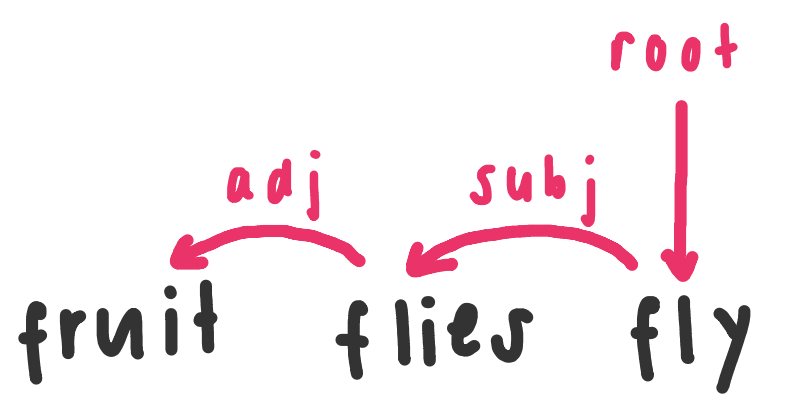
\includegraphics[height=10mm]{inhalt/images/NLP/06_dependency_parsing_1.png}
\\\\
\textit{2) Syntactic parsing $\to$ dependency parsing}\\
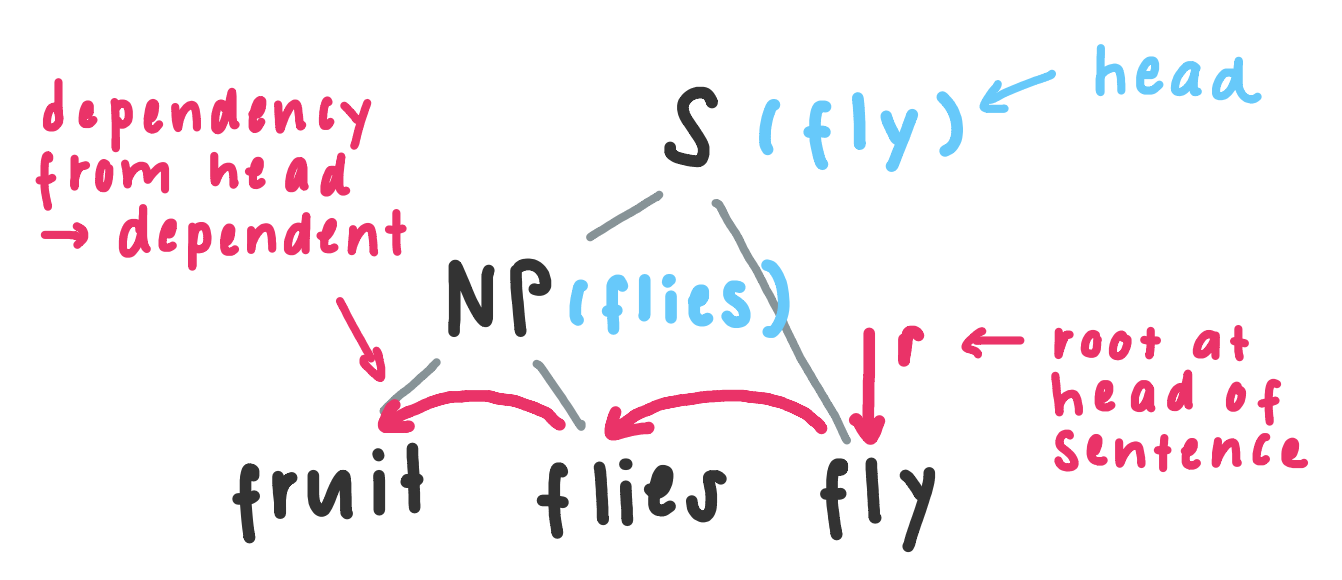
\includegraphics[height=10mm]{inhalt/images/NLP/06_dependency_parsing_2.png}
\end{multicols}
\section{Semantics | Semantic Parsing}
\subsection*{Description}
\emph{Task} --- Assign semantic structure, i.e. logical form, to a sentence

{\color{lightgray}\hrule height 0.001mm}

\emph{Description} ---
\begin{itemize}
    \item Principle of compositionality:
    \begin{itemize}
        \item The meaning of a complex expression is a function of the meanings of that expression's constituent parts
        \item $\rightarrow$ We can syntactically parse a sentence
        \item $\rightarrow$ We can then construct the semantic representation bottom-up
    \end{itemize}
    \item Applying the principle of compositionality:
    \begin{itemize}
        \item Syntactic rule, e.g. $\textrm{S} \to \textrm{NP VP}$
        \item Induces semantic rule, e.g. $\textrm{s.sem} \to \textrm{VP.sem} (\textrm{NP.sem})$: to get the semantic representation of sentence $s$, we apply the semantic representation of the verb phrase (a function) to the semantic representation of the noun phrase
    \end{itemize}
\end{itemize}

{\color{black}\hrule height 0.001mm}

\subsection*{Lambda Calculus}
\emph{Basics} ---
\begin{itemize}
    \item Basic terms: Variables $x, y, z, \dots$
    \begin{itemize}
        \item Free variables: Do not occur in the scope of any abstraction that holds its name
        \item Otherwise, bound variables: Bound by the abstraction with the smallest scope
        \item E.g. $((\textcolor{orange}{\lambda x[}.\textcolor{red}{\lambda y[}.(\textcolor{orange}{x} ((\textcolor{blue}{\lambda x.[x]} \textcolor{orange}{x}) \textcolor{red}{y}))\textcolor{red}{]}\textcolor{orange}{]} \textcolor{green}{\lambda x.[x]}) z)$ where
        \begin{itemize}
            \item $z$ is unbound
            \item Other variables are bound by same-colored abstractions
            \item Scopes of abstractions are indicated by square brackets
        \end{itemize}
    \end{itemize}
    \items New terms can be constructed using $2$ recursive rules:
    \begin{itemize}
        \item 1) Abstraction:
        \begin{itemize}
            \item If $M$ is a term, $N$ is a term, and $x$ is a variable:
            \begin{itemize}
                \item $\lambda x$ is an abstraction
                \item $\lambda x.M$ is a function that takes $x$ as input and produces $M$ as output by replacing every free occurrence of $x$ in $M$ with whatever the function is applied to (e.g. $N$)
                \item $\lambda x.M N$ is a function applied to $N$
                \item We denote the output of $\lambda x.M N$ as $M[x := N]$
                \item In the output of $\lambda x.M N$, only $M[x := N]$ remains, and $\lambda x.$ and $N$ disappear
            \end{itemize}
            \item Scope of abstraction: The scope of abstraction $\lambda x$ in expression $\lambda x.M$ is $M$
        \end{itemize}
        \item 2) Application: If $M$ and $N$ are terms, $(MN)$ is a term
    \end{itemize}
    \item Enriched lambda calculus offers additional components:
    \begin{itemize}
        \item Logical constants: Represent objects (e.g. Boston) and relationships (e.g. likes)
        \item Variables:
        \begin{itemize}
            \item Undetermined logical constants
            \item Objects are represented in lowercase as $x, y, z, \dots$ and are input to $\lambda x.f(x)$)
            \item Relations are represented in uppercase as $P, Q, R, \dots$ and are input to $\lambda P.P(\dots)$
        \end{itemize}
        \item Literals: Formed by applying relations to objects (e.g. likes(Alex, y), $P(x, y)$)
        \item Every relation symbol has an \emph{arity} that determines the number of objects it relates
        \item Logical connectives and quantifiers: $\exists, \forall, \neg, \land, \lor$
    \end{itemize}
\end{itemize}

{\color{lightgray}\hrule height 0.001mm}

\emph{Example} ---
\hl{INSERT IMAGE 1}

{\color{lightgray}\hrule height 0.001mm}

\emph{Alpha conversion} ---
\begin{itemize}
    \item Process of renaming a variable in a lambda term
    \item We can rename a variable in an abstraction together with all its occurrences in the scope of the abstraction, provided it remains bound to the same abstraction after renaming
    \item If the variable remains bound to the same abstraction, and no new variables become bound to the abstraction, the renaming is valid
    \item E.g. 
    $\lambda x.\lambda y.(x((\lambda x. x x) y )) \to \lambda z. \lambda y. (z((\lambda x. x z) y))$ is valid\\
    $\lambda x.(xy) \to \lambda y.(yy)$ is not valid, since $y$ was free before and is now bound
\end{itemize}

{\color{lightgray}\hrule height 0.001mm}

\emph{Beta reduction} ---
\begin{itemize}
    \item Process of applying one lambda term to another: $(\lambda x.M)N$
    \item We can apply one lambda term to another if the free variables in $N$ remain free in $M[x := N]$
    \item If this is not the case, first apply alpha-conversion to $M$
    \item Termination issue: Repeatedly applying beta reductions may not terminate
    \item E.g. $\lambda y.(z((\lambda x.\textcolor{blue}{\boldsymbol{x}}\textcolor{orange}{z})y)) \to \lambda y.(z(\textcolor{red}{z}y))$\\
    $(\lambda x.\textcolor{blue}{\lambda y.(\boldsymbol{x}((\lambda x.x\boldsymbol{x})y))}\textcolor{orange}{z}) \to \lambda y.(\textcolor{red}{z}((\lambda x.x\textcolor{red}{z})y))$
    where
    \begin{itemize}
        \item $\textcolor{blue}{blue}$ corresponds to $M$
        \item $\textcolor{orange}{orange}$ corresponds to $N$
        \item $\textcolor{red}{red}$ corresponds to $M[x := N]$
        \item $\boldsymbol{bold}$ corresponds to free variables in $M$
    \end{itemize}
\end{itemize}

{\color{lightgray}\hrule height 0.001mm}

\emph{Equivalence} --- Two lambda terms are equivalent if they can be obtained from each other via a series of $\alpha$- and $\beta$-conversions

{\color{black}\hrule height 0.001mm}

\subsection*{Combinatory Logic resp. SK-Calculus}
\begin{itemize}
    \item Alternative to lambda calculus
    \item Does not use abstractions
    \item Basic terms:
    \begin{itemize}
        \item Variables: $x, y, z, \dots$
        \item Primitive functions resp. combinators: $I, J, K, \dots$
        \begin{itemize}
            \item $I$ combinator: Identity function: $Ix = x$
            \item $K$ combinator: Constant function that always outputs $x$: $Kxy = ((Kx)y) = x$
            \item $S$ combinator: $Sxyz = (xz(yz)) = ((xz)(yz)$
        \end{itemize}
    \end{itemize}
    \item Terms are recursively constructed via application: If $M$ and $N$ are terms, $(MN)$ is a term
    \item Additional combinators:
    \begin{itemize}
        \item $B$ combinator resp. composition combinator: Composition function: $Bxyz = (x(yz))$
        \item $C$ combinator: $Cxyz = ((xz)y)$
        \item $T$ combinator resp. type-raising combinator: $Txy = yx$
    \end{itemize}
    \item Parentheses are left-associative, e.g. $(Kxyz) = (((Kx)y)z)$
    \item Reduction: 
    \begin{itemize}
        \item $SKK$ and $I$ are extensionally equivalent: $S(KK)x = SKKx = K x(K x) = x$
        \item Therefore, the $SK$ basis is complete, and we don't need $I$ operator
    \end{itemize}
\end{itemize}

{\color{black}\hrule height 0.001mm}

\subsection*{Transforming Lambda Calculus into SK-Calculus}
Apply recursively defined transformation $T$:
\begin{enumerate}
    \item $T(x) = x$ for every variable $x$
    \item $T[(E_1E_2)] = (T[E_1]T[E_2])$ for all lambda terms $E_1$ and $E_2$
    \item $T[\lambda x.E] = (KT[E])$ for every lambda term where $x$ is bound
    \item $T[\lambda x.x] =  (SKK) = I$
    \item $T[\lambda x.\lambda y.E] = T[\lambda x.T[\lambda y.E]]$ for every lambda term $E$ where $x$ is free
    \item $T[\lambda x.(E_1E_2)] = (ST[\lambda x.E_1]T[\lambda x.E_2])$ for all lambda terms $E_1, E_2$ where $x$ is free in at least one of the two terms
\end{enumerate}

{\color{black}\hrule height 0.001mm}

\subsection*{Linear Indexed Grammar resp. Combinatory Categorial Grammars (CCG)}
\emph{Features} --- 
\begin{itemize}
    \item Lexicalized grammar: Every word is associated with a syntactic category (including information about syntax and semantics) that defines how it combines with other words
    \item Compositionality: Semantic representation of a sentence is built in tandem with its syntactic derivation
    \item Flexible word order: Supports languages with complex or free word order (e.g. cross-serial dependencies, long-distance dependencies, coordination)
    \item The latter two are advantages over context-free grammars
\end{itemize}

{\color{lightgray}\hrule height 0.001mm}

\emph{Linear Indexed Grammar $\langle \mathcal{N}, S, \mathcal{I}, \Sigma, \mathcal{R} \rangle$} --- 
\begin{itemize}
    \item $\mathcal{N}$: Set of non-terminal symbols $N_1, N_2, N_3, \dots$
    \item $S$: Start non-terminal
    \item $\mathcal{I}$: Finite set of indices $f, g, h, \dots$
    \item $\Sigma$: Alphabet of terminal symbols $a_1, a_2, a_3, \dots$
    \item $\mathcal{R}$: Set of production rules of the following forms:
    \begin{itemize}
        \item $N[\sigma] \to \alpha M[\sigma]\beta$
        \item $N[\sigma] \to \alpha M[f\sigma]\beta$
        \item $N[f\sigma] \to \alpha M[\sigma]\beta$
        \item Where
        \begin{itemize}
            \item $N$ and $M$ are non-terminals
            \item $\alpha$ and $\beta$ are strings of terminals and non-terminals
            \item $\sigma$ is the stack passed to exactly one non-terminal on RHS
        \end{itemize}
    \end{itemize}
\end{itemize}

{\color{lightgray}\hrule height 0.001mm}

\emph{Combinatory Categorial Grammar $\langle \mathcal{V}_T, \mathcal{V}_N, S, f, \mathcal{R} \rangle$} --- 
\begin{itemize}
    \item $\mathcal{V}_T$: Set of terminals
    \item $\mathcal{V}_N$: Atomic categories: Set of non-terminals
    \item $S$: Start non-terminal $\in \mathcal{V}_N$
    \item $f: \mathcal{V}_T \to \mathcal{C}(\mathcal{V}_N)$: Lexicon: Function that maps elements of $\mathcal{V}_T \cup \{\varepsilon\}$ to finite subsets of $\mathcal{C}(\mathcal{V}_N)$, where $\mathcal{C}(\mathcal{V}_N)$ is the set of categories
    \item $\mathcal{R}$: Set of production rules, e.g. application
\end{itemize}
Composed of $2$ parts:
\begin{itemize}
    \item Lexicon: Associates words with categories, which encode the structure\\
    $\rightarrow$ Difference to context-free grammar, which encodes the structure in the rules
    \begin{itemize}
        \item Atomic categories: 
        \begin{itemize}
            \item Category of complete constituents
            \item E.g. $\textrm{Harry} := \boldsymbol{NP}$
        \end{itemize}
        \item Complex categories:
        \begin{itemize}
             \item Built recursively from atomic categories via operators
            \item Category of incomplete constituents
            \item Function that specifies the type of result and type and direction of its arguments
            \item E.g. $\textrm{walks} := (\textbf{S} \backslash \textbf{NP})$.
        \end{itemize}
        \item Set of categories $\mathcal{C}(\mathcal{V}_N)$ is the smallest set such that:
        \begin{itemize}
            \item If $C \in \mathcal{V}_N$, then $C \in \mathcal{C}(\mathcal{V}_N)$
            \item If $C_1, C_2 \in \mathcal{V}_N$, then $(C_1 / C_2) \in \mathcal{C}(\mathcal{V}_N)$ and $(C_1 \backslash C_2) \in \mathcal{C}(\mathcal{V}_N)$
        \end{itemize}
        \item Every category can be written in the form $X = A \mid_m X_m \dots \mid_1 X_1, \quad m \geq 0$ where
        \begin{itemize}
            \item $A$: Atomic category = target of $X$
            \item $X_1, \dots, X_m$: Arbitrary categories = arguments of $X$
            \item $\mid$ = Backward or forward slash
            \item $m$ = Arity of $X$
        \end{itemize}
    \end{itemize}
    \item Rules:
    \begin{itemize}
        \item Specify how categories can be combined into other categories
        \item Pattern: $X / Y \quad Y \to X$ where $X / Y$ is function, $Y$ is argument, and $X$ is result
        \item Types of rules:
        \begin{itemize}
            \item Function application:
            \begin{itemize}
                \item Forward application: $(>)$: If a category expects an argument to the right of $(X / Y)$ and argument $Y$ is available, they combine to form $X$: $X / Y \quad Y \to X$
                \item Backward application: $(<)$: If a category expects an argument to the left of $(X \backslash Y)$ and argument $Y$ is available, they combine to form $X$: $Y \quad X \backslash Y\to X$
                \item AB grammar resp. basic categorical grammar resp. pure categorical grammar:
                \begin{itemize}
                    \item CCGs that only have application rules
                    \item Have power of CFG:
                    $
                    A \to a \text{ in CCG} \equiv A \to a \text{ in CFG}
                    $\\
                    $
                    A \to (A / C) C \text{ in CCG} \equiv A \to BC \text{ in CFG}
                    $
                \end{itemize}
            \end{itemize}
            \item Function composition
            \begin{itemize}
                \item Two functions combine to form a single function: $f, g \to f \circ g$
                \item Forward composition: $((B_>$: $(X / Y) \quad (Y / Z) \to (X / Z)$
                \item Backward composition: $((B_<)$: $(Y \backslash Z) \quad (X \backslash Y) \to (X \backslash Z)$
            \end{itemize}
            \item Higher-order rules:
            \begin{itemize}
                \item Forward: $(>^n)$
                $
                X/Y \ Y \mid_n Y_n ... \mid_1 Y_1 \to X \mid_n Y_n ... \mid_1 Y_1 
                $
                \item Backward: $(<^n)$
                $
                Y \mid_n Y_n ... \mid_1 Y_1 \ X \backslash Y \to X \mid_n Y_n ... \mid_1 Y_1 
                $
                \item $n$ is the \emph{degree} of the rule
                \item If $n=0$, corresponds to application rule
            \end{itemize}
            \item Type raising:
            \begin{itemize}
                \item Turn an atomic category into a complex category so it can participate in higher-order functions
                \item Forward Type Raising: $(T_>)$
                $
                X \to T / (T \backslash X)
                $
                \item Backward Type Raising: $(T_<)$
                $
                X \to T \backslash (T / X)
                $
                \item E.g.:
                \begin{itemize}
                    \item Intransitive $\textrm{S} \backslash \textrm{NP}$ (e.g. walked)
                    \item Transitive $(\textrm{S} \backslash \textrm{NP}) / \textrm{NP}$ (e.g. respected)
                    \item Ditransitive $((\textrm{S} \backslash \textrm{NP}) / \textrm{NP}) / \textrm{NP}$ (e.g. gave)
                \end{itemize}
            \end{itemize}
        \end{itemize}
        \item Operators:
        \begin{itemize}
            \item Backward slash: $X \backslash Y$: "Give me a $Y$ to my left, and I return an $X$", means that function looks for argument to its left
            \item Forward slash: $X / Y$: "Give me a $Y$ to my right, and I return an $X$", means that function looks for argument to its right
            \item Operators need to be read from outside in, e.g. $(\textrm{S} \backslash \textrm{NP}) / \textrm{NP}$:
            \begin{itemize}
                \item Needs $\textrm{NP}$ to its right
                \item Then needs $\textrm{NP}$ to its left
                \item Then produces sentence $\textrm{S}$
            \end{itemize}
        \end{itemize}
        \item Rule instance is obtained by substituting $X, Y, Z, \dots$ by concrete categories, e.g. $\textrm{S, NP, VP}$, etc.
        \item CCGs have finite rules ($2^n$ forward, $2^n$ backward rules) and, thus, of non-terminals but infinitely many rule instances
    \end{itemize}
\end{itemize}
CCG parsing:
\begin{itemize}
    \item Deductive process
    \item General rule of inference:
    $
    \frac{A_1 \quad \dots \quad A_k}{B}
    $
    where $B$ is a consequence of $A_1, \dots, A_k$
    \item Derivation trees:
    \begin{itemize}
        \item Consist of unary and binary branches:
        \begin{itemize}
            \item Unary branches: Lexicon entries
            \item Binary branches: Composition rules:
            \begin{itemize}
                \item Can have primary and secondary input:
                \begin{itemize}
                    \item Primary input: Function of rule
                    \item Secondary input: Argument of rule
                    \item E.g. $X/Y \ Y\beta \to X\beta$ where $X/Y$ is primary input and $Y\beta$ is secondary input
                \end{itemize}
            \end{itemize}
            \item Structure:
            \hl{INSERT IMAGE 2}
        \end{itemize}
    \end{itemize}
\end{itemize}
CKY-style parsing algorithm:
\begin{itemize}
    \item Let $w$ be the sentence to be parsed, $w_i$ be a token in the sentence, and $w[i, j]$ be the substring from $w_{i+1} \dots w_j$, and $w_{ii} = \varepsilon$
    \item Aim: Construct item $[S, 0, n]$
    \item Derivation tree leading to this outcome has internal nodes $[X, i, j]$
    \item Axioms: $[x, i, i+1]$ where $w_{i+1} = x$ is a lexicon entry
    \item Inference rules:
    \begin{itemize}
        \item Forward:
        $
        \frac{[X / Y, i, j] \quad [Y \beta, j, k]}{[X \beta, i, k]} \quad X / Y \quad Y \beta \to X \beta
        $
        \item Backward:
        $
        \frac{[Y \beta, i, j] \quad [X \backslash Y, j, k]}{[X \beta, i, k]} \quad Y \beta \quad X \backslash Y \to X \beta
        $
    \end{itemize}
    \item Challenge: With the composition rule, we can grow the arity of the primary input categories and get exponentially many primary input categories
    \item Solution: Restrict the arity of the categories
\end{itemize}
Polynomial time algorithm:
\begin{itemize}
    \item Arity of categories is bounded by grammar constant $C_g$:
    $[X, i, j]$ where $\textrm{ar}(X) \leq C_g$
    \item Challenge: Categories with arity $> C_g$ can no longer be derived
    \item Solution:
    \begin{itemize}
        \item Introduce new rules that decompose longer derivations into smaller pieces
        \item Derivation context:
        \begin{itemize}
            \item None of the combinatory rules used in $c$ touches $X$, i.e. $c$ may pop and push the argument $Y$, but never touches $X$
            \item For this reason, $c$ is a derivation context and can be used for any category $X$ across multiple derivations
            \item \hl{INSERT IMAGE 3}
        \end{itemize}
        \item New items:
        \begin{itemize}
            \item $[\mid Y, \beta, i, i', j, j']$ where $\text{ar}(Y \beta) \leq C_g$
            \item For any category $X$, if we can build a derivation tree $t'$ with yield $w[i', j']$ and type $X \mid Y$, then we can build $t$ with yield $w[i, j]$ and type $X \beta$
            \item Derivation context $C$ can be combined with any $t'$ with item of form $[X \mid Y, i', j']$
            \item $c$ can have any internal structure, as long as $X$ is untouched
            \item $t'$ can have any internal structure, only positions $i',j'$ and argument $/Y$ matter for combination with $c$
        \end{itemize}
        \item New inference rules:
        \begin{itemize}
            \item Context items are derived when the composition of two categories would result in a category with arity $> C_g$:
            $
            \frac{[X / Y, i, j] \quad [Y \beta, j, k]}{[\mid Y, \beta, i, i, j, k}
            $ 
            where
            \begin{itemize}
                \item $X \mid Y \quad Y\beta \to X\beta$
                \item $\text{ar}(X \beta) > C_g$
            \end{itemize}
            \item For denominator of above equation:
            \begin{itemize}
                \item When the arity of the context is small enough, it can be recombined with the original derivation:
                $
                \frac{[X \mid Y, i', j'] \quad [\mid Y, \beta, i, i', j', j]}{[X \beta, i, j]}
                $ where $\text{ar}(X \beta) \leq C_g$
                \item Contexts can be extended similar to derivation trees:
                $
                \frac{[\mid Y, \beta / Z, i, i', j', j] \quad [Z_\gamma, j, k,]}{[\mid Y, \beta_\gamma, i, i', j', k]}
                $ where $\beta_\gamma$ refers to $\beta$ without $/ Z$ (can be $\varepsilon$) and where 
                \begin{itemize}
                    \item $X / Z \quad Z_\gamma \to X_\gamma$
                    \item $\text{ar}(Y \beta_\gamma) \leq C_g$
                \end{itemize}\\
                resp.
                $
                \frac{[Z_\gamma, i, j] \quad [\mid Y, \beta \backslash Z, j, j', k', k]}{[\mid Y, \beta_\gamma, i, j', k', k]} 
                $ where $\beta_\gamma$ refers to $\beta$ without $/ Z$ (can be $\varepsilon$) and where 
                \begin{itemize}
                    \item $Z_\gamma \quad X \backslash Z \to X_\gamma$
                    \item $\text{ar}(Y \beta_\gamma) \leq C_g$
                \end{itemize}
                \item For denominator of above equations:
                \begin{itemize}
                    \item If the context extended in this way has arity $> C_g$, a new context is derived from the previous context:
                    $
                    \frac{[\mid Y, \beta / Z, i, i', j', j] \quad [Z_\gamma, j, k]}{[\backslash Z, \gamma, i, i, j, k]}
                    $
                    \item When the arity of the extended context is small enough, it can be recombined with the original context:
                    $
                    \frac{[\mid_1 Y, \beta \mid_2 Z, i'', i', j', j''] \quad [\mid_2 Z, \gamma, i, i'', j'', j]}{[\mid_1 Y, \beta, i, i', j', j]}
                    $
                \end{itemize}
            \end{itemize}
        \end{itemize}
    \end{itemize}
    \item Grammar constant $C_g$ is at least as large as maximum arity of category in axioms $= \ell$ (e.g. if "likes" is in axioms, $C_g \geq 2$)
    \item Grammar constant $C_g$ is at least as large as maximal $Y$ (determined by largest arity $a$ in lexicon) and $\beta$ (determined by the maximum degree $n$ of composition rules), since we need to restrict the size of $Y \beta$
    \item Together: $C_g \geq \max \{ \ell, a + n \}$
\end{itemize}
CCG combine syntactic and semantic information when paired with lambda calculus:
\begin{itemize}
    \item E.g.\\
    Mary $:= \textrm{NP} : \textrm{MARY}(x)$\\
    likes $:= (\textrm{S} \backslash \textrm{NP}) / \textrm{NP} : \lambda x.\ \lambda y.\ \textrm{likes}(x, y)$\\
    natural language $:=$ syntax $:$ semantics
    \item If we parse a sentence syntactically, we can derive semantics bottom-up in the same order
    \item hl{INSERT IMAGE 4}
\end{itemize}
\section{Weighted Finite State Automata (WFSA)}
\subsection*{Finite State Automata (FSA)}
\emph{Task} --- Determine whether a string is an element of a given language

{\color{lightgrey}\hrule height 0.001mm}

\emph{Formalization} --- 
\begin{itemize}
    \item $\mathcal{A}$ is a 5-tuple $(\Sigma, Q, I, F, \delta)$
    \begin{itemize}
        \item $\Sigma$ is an alphabet
        \item $Q$ is a finite set of states
        \item $I \subseteq Q$ is the set of initial states
        \item $F \subseteq Q$ is the set of final or accepting states
        \item $\delta \subseteq Q \times (\Sigma \cup \{\varepsilon\}) \times Q$ resp. $q \xrightarrow{a \in \Sigma \cup \{\varepsilon\}} q'$ is a finite multiset of transitions from one state in $Q$ to another state in $Q$ via a symbol in $\Sigma$ 
    \end{itemize}
    \item Can be represented as a directed, possibly cyclical graph:
    \hl{INSERT IMAGE 1}
    \item Sequentially reads individual symbols of an input string $s$ and transitions from state $q$ to state $q'$ upon reading a symbol $a$ iff $(q, a, q') \in \delta$
    \item If the automaton, after reading the last symbol of $s$, ends up in a state $q_f \in F$, the automaton accepts the string
\end{itemize}

{\color{black}\hrule height 0.001mm}

\subsection*{Weighted Finite State Automata (WFSA)}
\begin{itemize}
    \item Generalization of FSA, where transitions are weighted with a semiring
    \item Unweighted FSA corresponds to WFSA weighted with Boolean semiring
    \item Formalization: $\mathcal{A}$ is a 7-tuple $(\Sigma, Q, I, F, \delta, \lambda, \rho)$ over a semiring $\mathcal{W} = (\mathbb{K}, \oplus, \otimes, 0, 1)$.
    \begin{itemize}
        \item $\Sigma$ is an alphabet
        \item $Q$ is a finite set of states
        \item $I = \{q \in Q \mid \lambda(q) \neq 0\} \subseteq Q$ is the set of initial states
        \item $F = \{q \in Q \mid \rho(q) \neq 0\} \subseteq Q$ is the set of final or accepting states
        \item $\delta \subseteq Q \times (\Sigma \cup \{\varepsilon\}) \times \mathbb{K} \times Q$ is a finite multiset of transitions from one state in $Q$ to another state in $Q$ via a symbol in $\Sigma$
        \item $\lambda : Q \to \mathbb{K}$ is an initial weighting function over $Q$
        \item $\rho : Q \to \mathbb{K}$ is a final weighting function over $Q$
    \end{itemize}
    \item Can be represented as a directed, possibly cyclical graph:
    \hl{INSERT IMAGE 2}
\end{itemize}

{\color{black}\hrule height 0.001mm}

\subsection*{(W)FSA Terminology}
\begin{itemize}
    \item Paths:
    \begin{itemize}
        \item A path $\pi$ is an element of $\delta^*$ with consecutive transitions:
        $
        q_1 \xrightarrow{a_1} q_2 \xrightarrow{a_2} q_3 \cdots q_{N-1} \xrightarrow{a_N} q_N
        $
        \item $\textrm{p}(\pi) = q_1$ is the beginning state of the path
        \item $\textrm{q}(\pi) = q_N$ is the ending state of the path
        \item Length of path $|\pi|$ is the number of transitions
        \item Yield of path $s(\pi)$ is the concatenation of symbols on the path
        \item Path sets: Denoted by capital $\Pi$
        \begin{itemize}
            \item $\Pi(\mathcal{A})$: Set of all paths in the automaton
            \item $\Pi(s, \mathcal{A})$: Set of all paths with yield $s$
            \item $\Pi(q, \mathcal{A})$: Set of all paths starting at $q$
            \item $\Pi(q, q', \mathcal{A})$: Set of all paths from $q$ to $q'$
            \item $\Pi(q, s, q', \mathcal{A})$: Set of all paths from $q$ to $q'$ with yield $s$
            \item $\Pi(\mathcal{Q}, \mathcal{A}) = \bigcup_{q \in Q} \Pi(q)$
            \item $\Pi(\mathcal{Q}, \mathcal{Q}', \mathcal{A}) = \bigcup_{q \in Q, q' \in Q'} \Pi(q, q')$
            \item $\Pi(\mathcal{Q}, s, \mathcal{Q}' \mathcal{A}) = \bigcup_{q \in Q, q' \in Q'} \Pi(q,s,q')$
        \end{itemize}
    \end{itemize}

    \item Cycles:
    \begin{itemize}
        \item A path is a cycle if starting and finishing states are the same
        \item A path contains a cycle if the same state appears multiple times
    \end{itemize}

    \item Transitions:
    \begin{itemize}
        \item Outgoing arcs from $q$: $E \mathcal{A} (q) = \{a, b, \ldots\ \mid (q, a, b, \ldots) \in \delta\}$
        \item Incoming arcs to $q$: $E^{-1} \mathcal{A} (q) = \{c, d, \ldots\ \mid (\ldots, c, d, q) \in \delta\}$
    \end{itemize}

    \item States:
    \begin{itemize}
        \item State $q$ is accessible iff $q \in I$ or there exists a path whose weight is not 0 from $I$ to $q$
        \item State $q$ is accessible iff $q \in F$ or there exists a path whose weight is not 0 from $q$ to $F$
    \end{itemize}

    \item (W)FSA is unambiguous iff for every string $s$ there is at most one accepting path
\end{itemize}

{\color{black}\hrule height 0.001mm}

\subsection*{(W)FSA Applications}
N-gram models, CRFs, HMMs can be represented with (W)FSAs

\emph{N-gram models} --- 
\begin{itemize}
    \item Let $\boldsymbol{y} = (y_1, \ldots, y_L)$ be a string with $y_1 = \textrm{BOS}$, $y_L = \textrm{EOS}$
    \item We want to model 
    $
    p(\boldsymbol{y}) = \prod_{n=1}^L p(y_n \mid y_{n-N+1}, \ldots, y_{n-1})
    $
    \item If we represent this with WFSA:
    \begin{itemize}
        \item States $Q$ represent all possible sequences of words of length $N$, i.e., all possible N-grams
        \item There are $m + |V|^{n-1} + 1$ states for an N-gram:
        \begin{itemize}
            \item 1 end state
            \item $|V|^{n-1}$ intermediate states
            \item $m = \begin{cases} 
                |V|^{n-2} & \textrm{for N-grams with } n \geq 2 \\ 
                0 & \textrm{for unigrams} 
            \end{cases}$
        \end{itemize}
        \item Transitions between states represent transitions from one N-gram to another \item Only transitions between N-grams which can follow each other are allowed, e.g.
        $
        y_{-N} \ y_{-N+1} \dots y_{-1}
        $
        and 
        $
        y_{-N+1} \ y_{-N+2} \dots y_{0}
        $
        receive weights $> 0$, with the weight representing the probability of observing the new word $y_0$ given the starting N-gram
    \end{itemize}
    \item Formalization:
    \begin{itemize}
        \item $\Sigma = \mathbb{Y} \cup \{\langle \textrm{BOS} \rangle, \langle\textrm{EOS} \rangle\}$
        \item $Q = \bigcup_{n=0}^N \{\langle \textrm{BOS} \rangle\}^{N-n} \times \mathbb{Y}^{n-1} \times (\mathbb{Y} \cup \{\langle \textrm{EOS} \rangle\})$
        \item $I = \{\langle \textrm{BOS}, \ldots, \textrm{BOS} \rangle\}$ ($N$ times)
        \item $F = Q$
        \item $\delta = \big\{ (y_{-N} \ldots y_{-1}, y_0, p(y_0 \mid y_{-N+1}, \ldots, y_{-1}), y_{-N+1} \ldots y_0 ) \textrm{ for } (y_{-N+1} \ldots y_{-1}) \in \bigcup_{n=0}^{N-1} \{ \langle \textrm{BOS} \rangle \}^{N-1-n} \times \mathbb{Y}^n  \big\}
        $
        \\
        $
        \delta(q_{ij}, w, 1, q_{ki}) = 
        \begin{cases} 
            \log(p(w_m = k \mid w_{m-1} ) = i, \ldots, w_{m-n+1} = j)) & \textrm{if } w=k \\
            -\infty & \textrm{otherwise}
        \end{cases}
        $
        \item $\lambda = \langle \textrm{BOS} \rangle \ldots \langle \textrm{BOS} \rangle \to 1$ ($N$ times)\\
        $\lambda(q_{ij}) = \log(p(w_m = l \mid w_{m-1} = \textrm{BOS}, \ldots, w_{m-n+1} = \textrm{BOS}))$
        \item $\rho = y_{n-N+1} \ldots y_1 \ \langle \textrm{EOS} \rangle \to 1$\\
        $
        \rho(q_{ij}) = \log(p(w_m = \textrm{EOS} \mid w_{m-n} = i, \ldots, w_{m-n+1} = j))
        $
    \end{itemize}
\end{itemize}

{\color{lightgrey}\hrule height 0.001mm}

\emph{CRFs} --- 
\begin{itemize}
    \item Let $|\boldsymbol{x}| = L$ and $|\boldsymbol{y}| = M$
    $
    \textrm{score}(\boldsymbol{y}, \boldsymbol{x}) = \boldsymbol{w} \cdot \boldsymbol{f}(\boldsymbol{x}, \boldsymbol{y})
    $
    \item We assume $\boldsymbol{f}$ decomposes additively:
    $
    \boldsymbol{f}(\boldsymbol{x}, \boldsymbol{y}) = \sum_{n=2}^L f(y_n, y_{n-1}, \boldsymbol{x}, n)
    $
    \item We want to model:
    $
    p(\boldsymbol{y} \mid \boldsymbol{x}) = \frac{\exp(\textrm{score}(\boldsymbol{y}, \boldsymbol{x}))}{Z(\boldsymbol{x})} = \frac{\prod_{n=2}^L \exp(\boldsymbol{w} \cdot f(y_n, y_{n-1}, \boldsymbol{x}, n))}{Z(\boldsymbol{x})}
    $
    where
    $
    Z(\boldsymbol{x}) = \sum_{\boldsymbol{y}'} \exp(\textrm{score}(\boldsymbol{y}', \boldsymbol{x})) = \sum_{\boldsymbol{y}'} \prod_{n=2}^L \exp(\boldsymbol{w} \cdot f(y_n', y_{n-1}', \boldsymbol{x}, n))
    $
    \item $Z(\boldsymbol{x})$ can be computed via the pathsum algorithm, as a generalization of the backward algorithm
    \item If we represent this with WFSA:
    \begin{itemize}
        \item States $Q$ represent all hidden states
        \item Transitions between states represent CRF scores assigned to hidden state $y'$ after hidden state $y$, given input sequence $\boldsymbol{x}$
    \end{itemize}
    \item Formalization:
    \begin{itemize}
        \item $\Sigma = \{\varepsilon\}$
        \item $Q = \mathbb{Y}^M$
        \item $I = Q$
        \item $F = Q$
        \item $\delta = \{(y_n, \varepsilon, \exp(\boldsymbol{w} \cdot f(y_n, y_{m}, \boldsymbol{x})), y_m) \}$
        \item $\lambda = y_n \to \exp(\boldsymbol{w} \cdot f(y_n, \langle \textrm{BOS} \rangle, \boldsymbol{x}))$
        \item $\rho = y_n \to \exp(\boldsymbol{w} \cdot f(\langle \textrm{EOS} \rangle, y_n, \boldsymbol{x}))$
    \end{itemize}
\end{itemize}

\emph{HMMs} --- 
\hl{TBA}

{\color{black}\hrule height 0.001mm}

\subsection*{Weighted Finite State Transducers (WFST)}
\emph{Task} --- Transforms input string in a given language to output string in a given language

{\color{lightgrey}\hrule height 0.001mm}

\emph{Formalization} --- 
\begin{itemize}
    \item $\mathcal{T}$ is an 8-tuple $(\Sigma, \Omega, Q, I, F, \delta, \lambda, \rho)$ over a semiring $\mathcal{W} = (\mathbb{K}, \oplus, \otimes, 0, 1)$
    \begin{itemize}
        \item $\Sigma$ is the input alphabet, containing letters or symbols
        \item $\Omega$ is the output alphabet, containing letters or symbols
        \item $Q$ is a finite set of states
        \item $I = \{q \in Q \mid \lambda(q) \neq 0\} \subseteq Q$ is the set of initial states
        \item $F = \{q \in Q \mid \rho(q) \neq 0\} \subseteq Q$ is the set of final or accepting states
        \item $\delta \subseteq Q \times (\Sigma \cup \{\varepsilon\}) \times (\Omega \cup \{\varepsilon\}) \times \mathbb{K} \times Q$ is a finite multiset of transitions from one state in $Q$ to another state in $Q$ via a symbol in $\Sigma$ and in $\Omega$
        \item $\lambda : Q \to \mathbb{K}$ is an initial weighting function over $Q$
        \item $\rho : Q \to \mathbb{K}$ is a final weighting function over $Q$
    \end{itemize}
    \item Furthermore:
    \begin{itemize}
        \item $s$: String over alphabet
        \item $\varepsilon$: Empty string
        \item $\Sigma^0 = \{\varepsilon\}$
        \item $\Sigma^* = \{\varepsilon, \ldots\}$ is the set of all possible strings (incl. the empty string $\varepsilon$) that can be formed by concatenation of 0 or more elements from $\Sigma$ 
        \item $L$: String language over an alphabet, subset of $\Sigma^*$, containing words
        \item $\boldsymbol{x}$: Input string
        \item $\boldsymbol{y}$: Transliteration of input string
    \end{itemize}
    \item Can be represented as a directed, possibly cyclical graph
    \hl{INSERT IMAGE 3}
\end{itemize}

{\color{black}\hrule height 0.001mm}

\subsection*{Compositions}
\begin{itemize}
    \item Operation to combine two or more WFSTs
    \item $\mathcal{T}_1 \circ \mathcal{T}_2$ is the composition of $\mathcal{T}_1 = (\Sigma, \Omega, Q_1, I_1, F_1, \delta_1, \lambda_1, \rho_1)$ and $\mathcal{T}_2 = (\Omega, \Gamma, Q_2, I_2, F_2, \delta_2, \lambda_2, \rho_2)$ and is given by:
    $
    \mathcal{T} = (\Sigma, \Gamma, Q, I, F, \delta, \lambda, \rho)
    $
    such that:
    $
    \mathcal{T}(x, y) = \bigoplus_{z \in \Omega^*} \mathcal{T}_1(x, z) \otimes \mathcal{T}_2(z, y)
    $
    \item Naive algorithm to compute composition:
    \begin{enumerate}
        \item $\mathcal{T} \gets (\Sigma, \Omega, Q, I, F, \delta, \lambda, \rho)$ to create a new WFST
        \item For $q_1, q_2 \in Q_1 \times Q_2$:\\
        For
        $
        (q_1 \xrightarrow{a:b/w_1} q_1'), (q_2 \xrightarrow{c:d/w_2} q_2') \in  E_{\mathcal{T}_1}(q_1) \times E_{\mathcal{T}_2}(q_2):
        $\\
        If $b=c$
        \begin{itemize}
            \item Add states $(q_1, q_2)$, $(q_1', q_2')$ to $\mathcal{T}$ if they have not yet been added
            \item Add arc $(q_1, q_2) \xrightarrow{a:d/w_1 \otimes w_2} (q_1', q_2')$ to $\mathcal{T}$
        \end{itemize}
        \item For $(q_1, q_2) \in Q$:
        \begin{itemize}
            \item $
            \lambda_\mathcal{T} = \lambda_1(q_1) \otimes \lambda_2(q_2)
            $
            \item $
            \rho_\mathcal{T} = \rho_1(q_1) \otimes \rho_2(q_2)
            $
        \end{itemize}
        \item Return $\mathcal{T}$
    \end{enumerate}
    \item Challenge: Runs through many useless states, has time complexity $\mathcal{O}(|Q_1||Q_2|)$
    \item Solution: Accessible algorithm
    \item Accessible algorithm:
    \begin{itemize}
        \item Intuition: Construct all possible pairs of initial states and then expand outwards (depth-first search), adding accessible states
        \item Attention: Produced states may still be non-co-accessible
        \begin{enumerate}
            \item $\textrm{stack} \gets [(q_1, q_2) \mid q_1 \in I_1, \, q_2 \in I_2]$ (ordered list, allows duplicates)\\
            $\textrm{visited} \gets \{(q_1, q_2) \mid q_1 \in I_1, \, q_2 \in I_2\}$ (unordered set, does not allow duplicates)
            \item $\mathcal{T} \gets (\Sigma, \Omega, Q, I, F, \delta, \lambda, \rho)$ to create a new WFST
            \item While $|\textrm{stack}| > 0$:
            \begin{itemize}
                \item $q_1, q_2 \gets \textrm{stack.pop()}$
                \item For:
                $
                (q_1 \xrightarrow{a:b/w_1} q_1'), \quad (q_2 \xrightarrow{c:d/w_2} q_2') \in E_{\mathcal{T}_1}(q_1) \times E_{\mathcal{T}_2}(q_2)$:\\
                If $b=c$:
                \begin{itemize}
                    \item Add states $(q_1, q_2)$, $(q_1', q_2')$ to $\mathcal{T}$ if they have not yet been added
                    \item Add arc $(q_1, q_2) \xrightarrow{a:d/w_1 \otimes w_2} (q_1', q_2')$ to $\mathcal{T}$
                    \item If $(q_1', q_2')$ not in visited:
                    \begin{itemize}
                        \item Push $(q_1', q_2')$ to stack and visited
                    \end{itemize}
                \end{itemize}
            \end{itemize}
            \item For $(q_1, q_2) \in Q$:
            \begin{itemize}
                \item $
                \lambda_\mathcal{T} = \lambda_1(q_1) \otimes \lambda_2(q_2)
                $
                \item $
                \rho_\mathcal{T} = \rho_1(q_1) \otimes \rho_2(q_2)
                $
            \end{itemize}
        \end{enumerate}
    \end{itemize}
    \item E.g.
    \hl{INSERT IMAGE 4}
\end{itemize}

{\color{black}\hrule height 0.001mm}

\subsection*{Transliteration}
\emph{Basics} ---
\begin{itemize}
    \item Mapping strings in one character set to strings in another character set E.g. $\textrm{Muse} \to \mu ou \sigma \alpha$
    \item Approach:
    \begin{enumerate}
        \item Design WFST $\mathcal{T}$ that maps string over $\Sigma$ to string over $\Omega$: $\mathcal{T}$ acts as a rule set
        \item Encode source sequence $\boldsymbol{x} \in \Sigma^*$ as WFST $\mathcal{T}_x$: Prepare $\boldsymbol{x}$ for alignment
        \item Compute normalizer $Z$ as pathsum of composition $\mathcal{T}_x \circ \mathcal{T}_y$: Compute denominator of $p(\boldsymbol{y} \mid \boldsymbol{x})$
        \item Encode target sequence $\boldsymbol{y} \in \Omega^*$ as WFST $\mathcal{T}_y$: Prepare $\boldsymbol{y}$ for alignment
        \item Sum over all possible alignments using pathsum of composition $\mathcal{T}_x \circ \mathcal{T} \circ \mathcal{T}_y$: Compute numerator of $p(\boldsymbol{y} \mid \boldsymbol{x})$
        \item Compute highest scoring path of composition $\mathcal{T}_x \circ \mathcal{T}$ using e.g. Dijkstra or Floyd-Warshall: Identify most probable transliteration
    \end{enumerate}
    \item How do we design $\mathcal{T}$? Path $\pi$ from $\mathcal{T}$'s initial states to a final state represents an alignment of $\boldsymbol{x}$ to $\boldsymbol{y}$
    \item How do we use training data?
    \begin{itemize}
        \item Dataset contains pairs $(\boldsymbol{x}, \boldsymbol{y})$, where sometimes there is an alignment between $\boldsymbol{x}$ and $\boldsymbol{y}$
        \item We treat the alignment as a latent variable
        \item If we represent $\boldsymbol{x}$ as transducer $\mathcal{T}_x$, the composition $\mathcal{T}_x \circ \mathcal{T}$ yields a new transducer whose paths correspond to the paths in $\mathcal{T}$ that have input $\boldsymbol{x}$: Each path in $\mathcal{T}_x \circ \mathcal{T}$ represents one alignment of $\boldsymbol{x}$ to some string in $\Omega^*$
        \item If we represent $\boldsymbol{y}$ as transducer $\mathcal{T}_y$, the composition $\mathcal{T}_x \circ \mathcal{T} \circ \mathcal{T}_y$ yields a new transducer whose paths correspond to the paths in $\mathcal{T}$ that align $\boldsymbol{x}$ to $\boldsymbol{y}$
        \item The probability $p(\boldsymbol{y} \mid \boldsymbol{x})$ is the total probability of all paths that align $\boldsymbol{x}$ to $\boldsymbol{y}$
    \end{itemize}
    \item How do we train? Maximize log-likelihood 
    $\sum_{\boldsymbol{x}, \boldsymbol{y} \in \mathcal{D}} \log p(\boldsymbol{y} \mid \boldsymbol{x}) = \textrm{pathsum of } \mathcal{T}_x \circ \mathcal{T} \circ \mathcal{T}_y, \textrm{ divided by pathsum of } \mathcal{T}_x \circ \mathcal{T}$
    \item How do we perform inference?
    \begin{itemize}
        \item Given $\boldsymbol{x}$
        \item Construct $\mathcal{T}_x \circ \mathcal{T}$, defining a probability distribution over all aligned $\boldsymbol{y}$
        \item If we condition on $\boldsymbol{x}$ in WFST $\mathcal{T}_x \circ \mathcal{T}$, this WFST becomes a WFSA
        \item Goal is then to find the highest scoring path in this graph
    \end{itemize}
    \item Why can't we use a CRF?
    \begin{itemize}
        \item In CRFs, we can only align sequences of the same length, e.g., $|\boldsymbol{x}| = |\boldsymbol{y}|$
        \item In WFSTs, we can align sequences of different lengths
    \end{itemize}
\end{itemize}

{\color{lightgrey}\hrule height 0.001mm}

\emph{Pathsum} ---
\begin{itemize}
    \item Inner path weight $w_\mid(\pi)$ of a path $\pi = q_0 \xrightarrow{a_1/w_1} q_1 \cdots q_{N-1} \xrightarrow{a_N/w_N} q_N$:
    $
    w_\mid(\pi) = \bigotimes_{n=1}^N w_n
    $
    \item Path weight $w(\pi)$ of a path:
    $
    w(\pi) = \lambda(\textrm{p}(\pi)) \otimes w_\mid \otimes \rho(\textrm{q}(\pi))
    $
    where $\textrm{p}(\pi)$ is the beginning state and $\textrm{q}(\pi)$ is the ending state
    \item A path is accepting or successful iff $w(\pi) \neq 0$
    \item String sum of a string $s \in \Sigma^*$ under $\mathcal{A}$:
    $
    A(s) = \bigoplus_{\pi \in \Pi(I, s, F)} w(\pi)
    $
    \item Path sum of $\mathcal{A}$:
    $
    Z(\mathcal{A}) = \bigoplus_{\pi \in \Pi(\mathcal{A})} w(\pi)
    $
    \item Path sum between two states $q_n, q_m$:
    $
    Z(q_n, q_m) = \bigoplus_{\pi \in \Pi(q_n, q_m)} w(\pi)
    $
    \item Path sum is equal to the shortest path weight, which can be seen, e.g., with the tropical semiring where $\otimes = +$ and $\oplus = \min$
    \item In a $\overline{0}$-closed semiring, the shortest path weight depends only on paths of length $N-1$, since paths of length $\geq N$ contain cycles, but cycles do not improve the path sum in $\overline{0}$-closed semirings, since $\overline{1} + a = \overline{1}$
    \item Challenge: There may be an infinite number of accepting paths (guaranteed if WFSA is cyclical)
    \item Nonetheless, we can compute the pathsum
    \item The pathsum problem subsumes several other problems:
    \begin{itemize}
        \item N-gram normalization
        \item CRF normalization
        \item Computing marginals in HMMs
    \end{itemize}
    \item Pathsum in acyclic WFSA:
    \begin{itemize}
        \item In acyclic WFSA, the number of accepting paths is finite
        \item To compute pathsum $Z(\mathcal{A})$, we need a topological sort of the nodes
        \item Backward algorithm:
        \begin{itemize}
            \item Computes $Z(\mathcal{A})$
            \begin{enumerate}
                \item For $q \in \textrm{Rev-Top}(\mathcal{A})$: (sorts nodes topologically)
                $
                \beta(q) = \rho(q) \oplus \bigoplus_{q \xrightarrow{a/w} q'} w \otimes \beta(q')
                $ i.e. proceeds in reverse topological order, $\oplus$-summing all weights of all paths coming from node $q$ and ending in final state $q_F$.
                \item Return:
                $
                \bigoplus_{q \in I} \lambda(q_\mid) \otimes \beta(q_\mid)
                $
            \end{enumerate}
            \item Runs in $\mathcal{O}(|\delta|)$ time and $\mathcal{O}(|Q|)$ space
            \item Could alternatively also be computed as forward algorithm. Then we would:
            \begin{itemize}
                \item Visit incoming edges (instead of outgoing)
                \item $\oplus$-add the initial weights (instead of final weights) in step (1)
                \item Post-$\otimes$-multiply the final weights (instead of initial weights) in step (2)
            \end{itemize}
        \end{itemize}
    \end{itemize}
    \item Pathsum in cyclical WFSA:
    \begin{itemize}
        \item In cyclical WFSA, the number of accepting paths is infinite
        \item To compute pathsum $Z(\mathcal{A})$, we need a closed semiring
        \item Lehmann algorithm:
        \begin{itemize}
            \item Computes $Z(\mathcal{A})$ by computing Kleene closure of matrixes over arbitraty closed semirings
            \item We must first represent WFSA as a matrix:
            \begin{itemize}
                \item Define $|\Sigma|$ \emph{adjacency matrices}, one for each transition symbol: $\boldsymbol{W}(a)$ is the adjacency matrix of transitions over $a$
                \item \hl{INSERT IMAGE 5}
                \item Since all paths are summed, we can collapse all transitions from $q_n$ to $q_m$ into a single transition without a label, whose weight is the $\oplus$-sum of all original transitions:
                $
                W(\mathcal{A}) = \bigoplus_{a \in \Sigma \cup \{\varepsilon\}} \boldsymbol{W}(a)
                $
            \end{itemize}
            \item Broad steps:
            \begin{enumerate}
                \item Lehmann algorithm computes the $\oplus$-sum over the path between two nodes $q_i, q_k$ with the matrix $\boldsymbol{W}$:
                $
                \boldsymbol{R}_{ik} = \bigoplus_{\pi \in \Pi(q_i, q_k)} w_\mid(\pi)
                $
                \begin{itemize}
                    \item Cyclical terms in calculation of $\boldsymbol{R}_{ik}$ are denoted with $*$
                    \item $\boldsymbol{R}_{ik}$ has $|Q|^2$ entries
                \end{itemize}
                \item From $\boldsymbol{R}$, we can compute $Z(\mathcal{A})$:
                $
                Z(\mathcal{A}) = \bigoplus_{i,k=1}^{|Q|} \lambda(q_i) \otimes \boldsymbol{R}_{ik} \otimes \rho(q_k)
                $
            \end{enumerate}
            \item E.g.
            \hl{INSERT IMAGE 6}
            \item Intuition:
            \begin{itemize}
                \item Partition path $\pi$ between $q_i$ and $q_k$ into subsets of paths:
                $\boldsymbol{M}^{\leq j}(q_i, q_k)$ are paths that do not cross nodes with indices $> j$\\
                $\boldsymbol{R}_{ik}^{\leq j}$ is the pathsum for these paths
                \item Any path either crosses $j$ or not
                \item For paths that do not cross $j$: 
                \begin{itemize}
                    \item $
                    \pi \in \Pi^{\leq j-1}(q_i, q_k)
                    $
                    \item In that case, the pathsum is:
                    $
                    \boldsymbol{R}_{ik}^{\leq j-1}
                    $
                \end{itemize}
                \item For paths that do cross $j$: 
                \begin{itemize}
                    \item $\pi$ can be decomposed into cycle that starts and ends in $j$, part before cycle, and part after cycle: $
                    \pi = \pi_{ij} \pi_{jj} \pi_{jk}
                    $
                    \item In that case, we can also decompose the pathsum into partial pathsums:
                    $
                    \boldsymbol{R}_{ik}^{\leq j} = \boldsymbol{R}_{ij}^{\leq j-1} \otimes \boldsymbol{R}_{jj}^{\leq j-1 *} \otimes \boldsymbol{R}_{jk}^{\leq j-1}
                    $
                \end{itemize}
                \item This defines a natural procedure to build up the pathsum from the partial pathsums
                \item All that's left is the starting condition:
                $
                R^{\leq 0} = \boldsymbol{W}
                $ since $\boldsymbol{W}$ captures paths not passing through intermediary nodes
            \end{itemize}
            \item Algorithm:
            \begin{enumerate}
                \item $\boldsymbol{R}^{(0)} \gets \boldsymbol{W}$
                \item For $j \gets 1$ up to $|Q|$:\\
                For $i \gets 1$ up to $|Q|$:\\
                For $k \gets 1$ up to $|Q|$:
                $
                \boldsymbol{R}_{ik}^{(j)} \gets \boldsymbol{R}_{ik}^{(j-1)} \oplus \big(\boldsymbol{R}_{ij}^{(j-1)} \otimes \boldsymbol{R}_{jj}^{(j-1)*} \otimes \boldsymbol{R}_{jk}^{(j-1)}\big)
                $
                \item Return:
                $
                I \bigoplus \boldsymbol{R}^{(|Q|)}
                $
            \end{enumerate}
            \item E.g.
            \hl{INSERT IMAGE 7}
            \item Runs in $\mathcal{O}(|Q|^3)$ time
            \item Lehmann algorithm encompasses Floyd-Warshall algorithm and Gauss-Jordan algorithm
        \end{itemize}
    \end{itemize}
\end{itemize}

{\color{lightgrey}\hrule height 0.001mm}

\emph{Transliteration} ---
Pathsum in $\boldsymbol{x}$-conditioned WFSA:    \begin{itemize}
    \item Let $(\boldsymbol{x}, \boldsymbol{y})$ be an unaligned training pair
    \item $\mathcal{A}_x$ is the $\boldsymbol{x}$-conditioned WFSA:
    \begin{itemize}
        \item $\boldsymbol{\lambda}$ is a vector of start weights for starting states: $\lambda_n = \lambda(q_n)$
        \item $\boldsymbol{\rho}$ is a vector of end weights for ending states: $\rho_m = \rho(q_m)$
        \item Set of transition matrices $\boldsymbol{W}^{(\omega)}$ for any $\omega \in \Omega \cup \{\varepsilon\}$:
        $
        \boldsymbol{W}_{nm}^{(\omega)}$ is the weight for $q_n \xrightarrow{\omega} q_m
        $
        \item $\boldsymbol{W}^{(\omega)}$ can be summarized into a single matrix:
        $
        \boldsymbol{W} = \sum_{\omega \in \Omega \cup \{\varepsilon\}} \boldsymbol{W}^{(\omega)}
        $
    \end{itemize}
    \item For instance: Likelihood:
    $
    p(\boldsymbol{y} \mid \boldsymbol{x}) = \frac{\exp(\textrm{score}(\boldsymbol{x}, \boldsymbol{y}))}{Z(\boldsymbol{x})}
    $ 
    \item
    $
    \textrm{score}(\boldsymbol{x}, \boldsymbol{y}) = \log \sum_{\pi \in \Pi(\boldsymbol{y})} w(\pi)
    $
    \item Normalizing constant is the pathsum:
    $
    Z(\boldsymbol{x}) = \sum_{\boldsymbol{y}' \in \Omega^*} \exp(\textrm{score}(\boldsymbol{x}, \boldsymbol{y}'))
    $\\
    $
    = \sum_{\boldsymbol{y}' \in \Omega^*} \exp \Big( \log \sum_{\pi \in \Pi(\boldsymbol{y}')} w(\pi) \Big)
    $\\
    $
    = \sum_{\boldsymbol{y}' \in \Sigma^*} \sum_{\pi \in \Pi(\boldsymbol{y}')} \lambda(\textrm{p}(\pi)) \otimes w_\mid(\pi) \otimes \rho(\textrm{q}(\pi))
    $\\
    $
    = \sum_{\boldsymbol{y}' \in \Sigma^*} \sum_{\pi \in \Pi(\boldsymbol{y}')} \lambda(\textrm{p}(\pi)) \otimes \prod_{n=1}^{| \pi |} w_n(\pi) \otimes \rho(\textrm{q}(\pi))
    $ which is the pathsum\\
    $
    = \sum_{q_n, q_m \in Q} \Big( \sum_{\pi \in \Pi(q_n, q_m)} w(\pi) \Big)
    $\\
    $
    = \sum_{q_n, q_m \in Q} \sum_{\pi \in \Pi(q_n, q_m)} \lambda(\textrm{p}(\pi)) \otimes w_\mid(\pi) \otimes \rho(\textrm{q}(\pi))
    $\\
    $
    = \sum_{q_n, q_m \in Q} \sum_{\pi \in \Pi(q_n, q_m)} \lambda(q_n) \otimes w_\mid(\pi) \otimes \rho(q_m)
    $\\
    $
    = \sum_{q_n, q_m \in Q} \lambda(q_n) \otimes (\sum_{\pi \in \Pi(q_n, q_m)} w_\mid(\pi)) \otimes \rho(q_m)
    $\\
    $
    = \sum_{q_n, q_m \in Q} \lambda(q_n) \otimes (\boldsymbol{W}^*)_{nm} \otimes \rho(q_m)
    $\\
    $
    = \boldsymbol{\lambda}^\intercal \boldsymbol{W}^* \boldsymbol{\rho}
    $ where $\boldsymbol{W}$ can be computed via Lehmann
    \item For instance: Log-likelihood: $\log p(\boldsymbol{y} \mid \boldsymbol{x})$
    \item For a full training dataset: Log-likelihood: $\sum_{n=1}^N \log p(\boldsymbol{y}^{(n)} \mid \boldsymbol{x}^{(n)}) = \sum_{n=1}^N \Big[ \textrm{score}(\boldsymbol{y}^{(n)}, \boldsymbol{x}^{(n)}) - \log Z(\boldsymbol{x}^{(n)}) \Big]$
    \item This can be optimized with backpropagation (in $\mathcal{O}(|Q|^3)$) and gradient descent
    \item To train transliteration WFST, we use the log semiring
    \item To estimate the probability of the most likely transliteration $\boldsymbol{y}$ for a given input $\boldsymbol{x}$, we use the arctic semiring
\end{itemize}
\section{Reinforcement Learning for NLP}
\subsection*{Formulation}

$S$: States
\begin{itemize}
    \item $s = \mathcal{X} \times \mathcal{Y} = \{ \boldsymbol{x}, \tilde{\boldsymbol{y}} \}$, where $\boldsymbol{x}$ is input and $\tilde{\boldsymbol{y}}$ is partial output
\end{itemize}

$A$: Actions
\begin{itemize}
    \item Elementary modifications, e.g., adding a single edge to a dependency tree
\end{itemize}

$T$: Transition function
\begin{itemize}
    \item Specifies which state the agent will end up in if it commits a certain action in a certain state
    \item Transition corresponds to replacing the current partial output $\tilde{\boldsymbol{y}}$ with transformed partial output $a(\tilde{\boldsymbol{y}})$ after applying action $a$:
    $
    T(( \boldsymbol{x}, \tilde{\boldsymbol{y}} ), a) = ( \boldsymbol{x}, a(\tilde{\boldsymbol{y}}) )
    $
\end{itemize}

$r$: Reward function
\begin{itemize}
    \item Specifies the reward the agent obtains by committing a certain action in a certain state:
    $
    r(s = ( \boldsymbol{x}, a(\tilde{\boldsymbol{y}}) )) = -\big(\Delta(a(\tilde{\boldsymbol{y}}), \boldsymbol{y}) - \Delta(\tilde{\boldsymbol{y}}, \boldsymbol{y})\big)
    $ i.e.  -(loss after action - loss before action)
    where:
    \begin{itemize}
        \item $\Delta(a(\tilde{\boldsymbol{y}}), \boldsymbol{y})$ is the loss between the true output $\boldsymbol{y}$ and the new prediction after applying action $a$ to $\tilde{\boldsymbol{y}}$
        \item $\Delta(\tilde{\boldsymbol{y}}, \boldsymbol{y})$ is the loss between the true output $\boldsymbol{y}$ and the current prediction $\tilde{\boldsymbol{y}}$
    \end{itemize}
    \item Intuitively:
    \begin{itemize}
        \item If loss after action $>$ loss before action, $r$ is negative
        \item Otherwise, $r$ is positive
    \end{itemize}
\end{itemize}

$\pi$: Policy
\begin{itemize}
    \item Set of rules that tell the agent which action to take in a certain state
    \item Policy score: Distinguishes good from bad policies:
    $
    \eta(\pi, s) = \sum_{t=1}^T r(s_t, \pi(s_t)) \mid \pi, s_1 = s
    $
    where:
    \begin{itemize}
        \item Total reward for policy starting at $s = s_1$ is calculated by summing the reward at each time step
        \item $\pi(s_t)$ maps action $a_t$ to state $s_t$
        \item $r(s_t, \pi(s_t))$ is the reward of taking action $a_t$ in state $s_t$
        \item $T$ is the maximum number of steps allowed to transition from $s_1$ to a final valid output
    \end{itemize}
\end{itemize}

{\color{black}\hrule height 0.001mm}

\subsection*{Optimization}
Optimal policy search:
$
\pi^* = argmax_{\theta \in \Theta} \mathbb{E}_{s \sim \mathcal{D}}[\eta(\pi_\theta, s)]
$
\end{multicols*}
\end{document}